\documentclass[twoside]{book}

% Packages required by doxygen
\usepackage{fixltx2e}
\usepackage{calc}
\usepackage{doxygen}
\usepackage[export]{adjustbox} % also loads graphicx
\usepackage{graphicx}
\usepackage[utf8]{inputenc}
\usepackage{makeidx}
\usepackage{multicol}
\usepackage{multirow}
\PassOptionsToPackage{warn}{textcomp}
\usepackage{textcomp}
\usepackage[nointegrals]{wasysym}
\usepackage[table]{xcolor}

% Font selection
\usepackage[T1]{fontenc}
\usepackage[scaled=.90]{helvet}
\usepackage{courier}
\usepackage{amssymb}
\usepackage{sectsty}
\renewcommand{\familydefault}{\sfdefault}
\allsectionsfont{%
  \fontseries{bc}\selectfont%
  \color{darkgray}%
}
\renewcommand{\DoxyLabelFont}{%
  \fontseries{bc}\selectfont%
  \color{darkgray}%
}
\newcommand{\+}{\discretionary{\mbox{\scriptsize$\hookleftarrow$}}{}{}}

% Page & text layout
\usepackage{geometry}
\geometry{%
  a4paper,%
  top=2.5cm,%
  bottom=2.5cm,%
  left=2.5cm,%
  right=2.5cm%
}
\tolerance=750
\hfuzz=15pt
\hbadness=750
\setlength{\emergencystretch}{15pt}
\setlength{\parindent}{0cm}
\setlength{\parskip}{3ex plus 2ex minus 2ex}
\makeatletter
\renewcommand{\paragraph}{%
  \@startsection{paragraph}{4}{0ex}{-1.0ex}{1.0ex}{%
    \normalfont\normalsize\bfseries\SS@parafont%
  }%
}
\renewcommand{\subparagraph}{%
  \@startsection{subparagraph}{5}{0ex}{-1.0ex}{1.0ex}{%
    \normalfont\normalsize\bfseries\SS@subparafont%
  }%
}
\makeatother

% Headers & footers
\usepackage{fancyhdr}
\pagestyle{fancyplain}
\fancyhead[LE]{\fancyplain{}{\bfseries\thepage}}
\fancyhead[CE]{\fancyplain{}{}}
\fancyhead[RE]{\fancyplain{}{\bfseries\leftmark}}
\fancyhead[LO]{\fancyplain{}{\bfseries\rightmark}}
\fancyhead[CO]{\fancyplain{}{}}
\fancyhead[RO]{\fancyplain{}{\bfseries\thepage}}
\fancyfoot[LE]{\fancyplain{}{}}
\fancyfoot[CE]{\fancyplain{}{}}
\fancyfoot[RE]{\fancyplain{}{\bfseries\scriptsize Generated by Doxygen }}
\fancyfoot[LO]{\fancyplain{}{\bfseries\scriptsize Generated by Doxygen }}
\fancyfoot[CO]{\fancyplain{}{}}
\fancyfoot[RO]{\fancyplain{}{}}
\renewcommand{\footrulewidth}{0.4pt}
\renewcommand{\chaptermark}[1]{%
  \markboth{#1}{}%
}
\renewcommand{\sectionmark}[1]{%
  \markright{\thesection\ #1}%
}

% Indices & bibliography
\usepackage{natbib}
\usepackage[titles]{tocloft}
\setcounter{tocdepth}{3}
\setcounter{secnumdepth}{5}
\makeindex

% Hyperlinks (required, but should be loaded last)
\usepackage{ifpdf}
\ifpdf
  \usepackage[pdftex,pagebackref=true]{hyperref}
\else
  \usepackage[ps2pdf,pagebackref=true]{hyperref}
\fi
\hypersetup{%
  colorlinks=true,%
  linkcolor=blue,%
  citecolor=blue,%
  unicode%
}

% Custom commands
\newcommand{\clearemptydoublepage}{%
  \newpage{\pagestyle{empty}\cleardoublepage}%
}

\usepackage{caption}
\captionsetup{labelsep=space,justification=centering,font={bf},singlelinecheck=off,skip=4pt,position=top}

%===== C O N T E N T S =====

\begin{document}

% Titlepage & ToC
\hypersetup{pageanchor=false,
             bookmarksnumbered=true,
             pdfencoding=unicode
            }
\pagenumbering{alph}
\begin{titlepage}
\vspace*{7cm}
\begin{center}%
{\Large Jobber }\\
\vspace*{1cm}
{\large Generated by Doxygen 1.8.14}\\
\end{center}
\end{titlepage}
\clearemptydoublepage
\pagenumbering{roman}
\tableofcontents
\clearemptydoublepage
\pagenumbering{arabic}
\hypersetup{pageanchor=true}

%--- Begin generated contents ---
\chapter{Hierarchical Index}
\section{Class Hierarchy}
This inheritance list is sorted roughly, but not completely, alphabetically\+:\begin{DoxyCompactList}
\item \contentsline{section}{psql}{\pageref{classpsql}}{}
\item Q\+Dialog\begin{DoxyCompactList}
\item \contentsline{section}{connect\+Psql}{\pageref{classconnect_psql}}{}
\item \contentsline{section}{statistics}{\pageref{classstatistics}}{}
\end{DoxyCompactList}
\item Q\+Main\+Window\begin{DoxyCompactList}
\item \contentsline{section}{Main\+Window}{\pageref{class_main_window}}{}
\item \contentsline{section}{New\+City}{\pageref{class_new_city}}{}
\item \contentsline{section}{New\+Country}{\pageref{class_new_country}}{}
\item \contentsline{section}{New\+Job}{\pageref{class_new_job}}{}
\item \contentsline{section}{New\+Status}{\pageref{class_new_status}}{}
\item \contentsline{section}{Show\+Cities}{\pageref{class_show_cities}}{}
\item \contentsline{section}{Show\+Countries}{\pageref{class_show_countries}}{}
\item \contentsline{section}{Show\+Statuses}{\pageref{class_show_statuses}}{}
\item \contentsline{section}{Spesific\+Jobs}{\pageref{class_spesific_jobs}}{}
\item \contentsline{section}{View\+Jobs}{\pageref{class_view_jobs}}{}
\end{DoxyCompactList}
\item \contentsline{section}{string\+Check}{\pageref{classstring_check}}{}
\end{DoxyCompactList}

\chapter{Class Index}
\section{Class List}
Here are the classes, structs, unions and interfaces with brief descriptions\+:\begin{DoxyCompactList}
\item\contentsline{section}{\hyperlink{classconnect_psql}{connect\+Psql} \\*The \hyperlink{classconnect_psql}{connect\+Psql} class }{\pageref{classconnect_psql}}{}
\item\contentsline{section}{\hyperlink{class_main_window}{Main\+Window} \\*The \hyperlink{class_main_window}{Main\+Window} class }{\pageref{class_main_window}}{}
\item\contentsline{section}{\hyperlink{class_new_city}{New\+City} \\*The \hyperlink{class_new_city}{New\+City} class }{\pageref{class_new_city}}{}
\item\contentsline{section}{\hyperlink{class_new_country}{New\+Country} }{\pageref{class_new_country}}{}
\item\contentsline{section}{\hyperlink{class_new_job}{New\+Job} \\*The \hyperlink{class_new_job}{New\+Job} class }{\pageref{class_new_job}}{}
\item\contentsline{section}{\hyperlink{class_new_status}{New\+Status} \\*The \hyperlink{class_new_status}{New\+Status} class }{\pageref{class_new_status}}{}
\item\contentsline{section}{\hyperlink{classpsql}{psql} \\*The psql class }{\pageref{classpsql}}{}
\item\contentsline{section}{\hyperlink{class_show_cities}{Show\+Cities} \\*The \hyperlink{class_show_cities}{Show\+Cities} class }{\pageref{class_show_cities}}{}
\item\contentsline{section}{\hyperlink{class_show_countries}{Show\+Countries} }{\pageref{class_show_countries}}{}
\item\contentsline{section}{\hyperlink{class_show_statuses}{Show\+Statuses} \\*The \hyperlink{class_show_statuses}{Show\+Statuses} class }{\pageref{class_show_statuses}}{}
\item\contentsline{section}{\hyperlink{class_spesific_jobs}{Spesific\+Jobs} }{\pageref{class_spesific_jobs}}{}
\item\contentsline{section}{\hyperlink{classtestefil}{testefil} }{\pageref{classtestefil}}{}
\item\contentsline{section}{\hyperlink{class_view_jobs}{View\+Jobs} \\*The \hyperlink{class_view_jobs}{View\+Jobs} class }{\pageref{class_view_jobs}}{}
\end{DoxyCompactList}

\chapter{File Index}
\section{File List}
Here is a list of all documented files with brief descriptions\+:\begin{DoxyCompactList}
\item\contentsline{section}{{\bfseries connectpsql.\+h} }{\pageref{connectpsql_8h}}{}
\item\contentsline{section}{{\bfseries mainwindow.\+h} }{\pageref{mainwindow_8h}}{}
\item\contentsline{section}{\mbox{\hyperlink{newcity_8cpp}{newcity.\+cpp}} }{\pageref{newcity_8cpp}}{}
\item\contentsline{section}{{\bfseries newcity.\+h} }{\pageref{newcity_8h}}{}
\item\contentsline{section}{{\bfseries newcountry.\+h} }{\pageref{newcountry_8h}}{}
\item\contentsline{section}{{\bfseries newjob.\+h} }{\pageref{newjob_8h}}{}
\item\contentsline{section}{{\bfseries newstatus.\+h} }{\pageref{newstatus_8h}}{}
\item\contentsline{section}{\mbox{\hyperlink{psql_8cpp}{psql.\+cpp}} }{\pageref{psql_8cpp}}{}
\item\contentsline{section}{{\bfseries psql.\+h} }{\pageref{psql_8h}}{}
\item\contentsline{section}{{\bfseries showcities.\+h} }{\pageref{showcities_8h}}{}
\item\contentsline{section}{{\bfseries showcountries.\+h} }{\pageref{showcountries_8h}}{}
\item\contentsline{section}{{\bfseries showstatuses.\+h} }{\pageref{showstatuses_8h}}{}
\item\contentsline{section}{{\bfseries spesificjobs.\+h} }{\pageref{spesificjobs_8h}}{}
\item\contentsline{section}{{\bfseries statistics.\+h} }{\pageref{statistics_8h}}{}
\item\contentsline{section}{{\bfseries viewjobs.\+h} }{\pageref{viewjobs_8h}}{}
\end{DoxyCompactList}

\chapter{Class Documentation}
\hypertarget{classadvanced_search}{}\section{advanced\+Search Class Reference}
\label{classadvanced_search}\index{advancedSearch@{advancedSearch}}
Inheritance diagram for advanced\+Search\+:\begin{figure}[H]
\begin{center}
\leavevmode
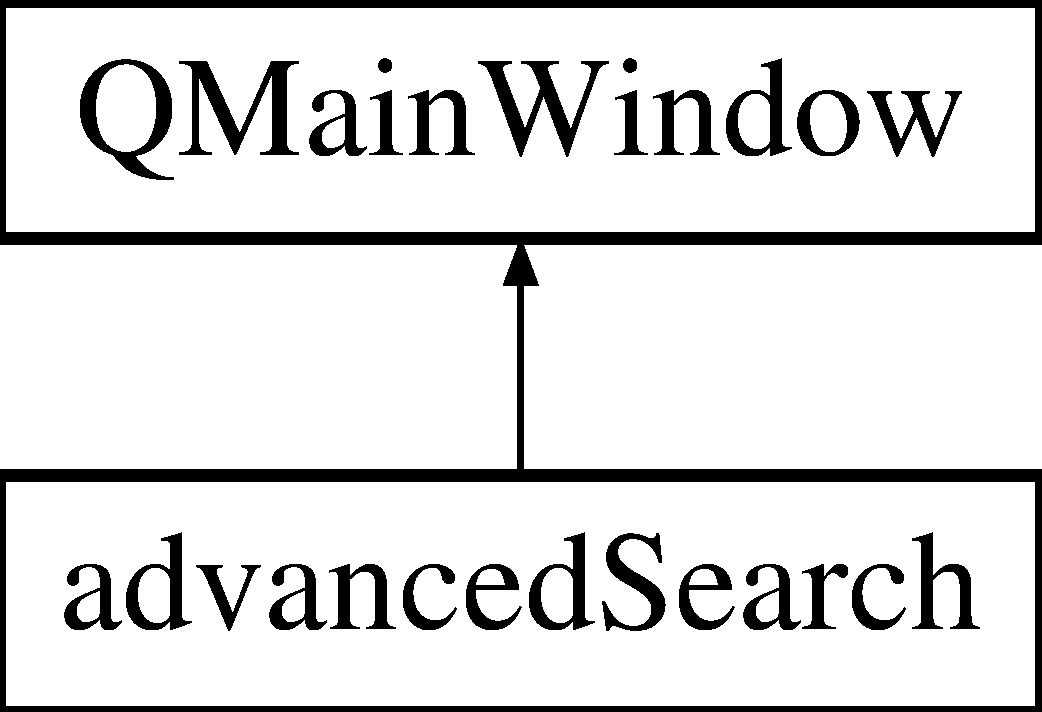
\includegraphics[height=2.000000cm]{classadvanced_search}
\end{center}
\end{figure}
\subsection*{Public Member Functions}
\begin{DoxyCompactItemize}
\item 
\mbox{\hyperlink{classadvanced_search_ae9e0253869871c6af23d804fdc78d184}{advanced\+Search}} (Q\+String title, \mbox{\hyperlink{classpsql}{psql}} $\ast$pg, Q\+Widget $\ast$parent=0)
\begin{DoxyCompactList}\small\item\em \mbox{\hyperlink{classadvanced_search_ae9e0253869871c6af23d804fdc78d184}{advanced\+Search\+::advanced\+Search}} \mbox{\hyperlink{classadvanced_search}{advanced\+Search}} class constructor \end{DoxyCompactList}\item 
Q\+String \mbox{\hyperlink{classadvanced_search_a7bcbaf1e2663396daacf9b033c34238a}{get\+Job\+Title}} ()
\begin{DoxyCompactList}\small\item\em \mbox{\hyperlink{classadvanced_search_a7bcbaf1e2663396daacf9b033c34238a}{advanced\+Search\+::get\+Job\+Title}} Gets the job title \end{DoxyCompactList}\item 
Q\+String \mbox{\hyperlink{classadvanced_search_a5e9e9e24e83f36f9ed32bd60cecbb7de}{get\+Company\+Name}} ()
\begin{DoxyCompactList}\small\item\em \mbox{\hyperlink{classadvanced_search_a5e9e9e24e83f36f9ed32bd60cecbb7de}{advanced\+Search\+::get\+Company\+Name}} Gets the company name \end{DoxyCompactList}\item 
Q\+String \mbox{\hyperlink{classadvanced_search_ae061d04a2d39bcb3dc363fc56752377b}{get\+City\+Name}} ()
\begin{DoxyCompactList}\small\item\em \mbox{\hyperlink{classadvanced_search_ae061d04a2d39bcb3dc363fc56752377b}{advanced\+Search\+::get\+City\+Name}} Gets the name of the city where the job is located \end{DoxyCompactList}\item 
Q\+String \mbox{\hyperlink{classadvanced_search_afc318495c6475695844bd0f22c6c1e3c}{get\+Status}} ()
\begin{DoxyCompactList}\small\item\em \mbox{\hyperlink{classadvanced_search_afc318495c6475695844bd0f22c6c1e3c}{advanced\+Search\+::get\+Status}} Gets the status of the job application \end{DoxyCompactList}\item 
Q\+String \mbox{\hyperlink{classadvanced_search_ae58a90dea341fa431df72e368b70267e}{get\+Deadline}} ()
\begin{DoxyCompactList}\small\item\em \mbox{\hyperlink{classadvanced_search_ae58a90dea341fa431df72e368b70267e}{advanced\+Search\+::get\+Deadline}} Gets the deadline of the application \end{DoxyCompactList}\item 
Q\+String \mbox{\hyperlink{classadvanced_search_a40af6df4af92bc7f4cff89729df2c6da}{get\+Motivation}} ()
\begin{DoxyCompactList}\small\item\em \mbox{\hyperlink{classadvanced_search_a40af6df4af92bc7f4cff89729df2c6da}{advanced\+Search\+::get\+Motivation}} Gets the motivation for applying for this job. \end{DoxyCompactList}\item 
void \mbox{\hyperlink{classadvanced_search_a698024f20a64fd27b1b352bce5c6f527}{set\+Job\+Title}} (Q\+String new\+Title)
\begin{DoxyCompactList}\small\item\em \mbox{\hyperlink{classadvanced_search_a698024f20a64fd27b1b352bce5c6f527}{advanced\+Search\+::set\+Job\+Title}} Sets the title of the job \end{DoxyCompactList}\item 
void \mbox{\hyperlink{classadvanced_search_a6d817d740d8e614bf93cec866735bd7f}{set\+Company\+Name}} (Q\+String new\+Name)
\begin{DoxyCompactList}\small\item\em \mbox{\hyperlink{classadvanced_search_a6d817d740d8e614bf93cec866735bd7f}{advanced\+Search\+::set\+Company\+Name}} Sets the name of the company \end{DoxyCompactList}\item 
void \mbox{\hyperlink{classadvanced_search_a285bcf54a61d42fa81a7d1a5a86c5779}{set\+City\+Name}} (Q\+String new\+City\+Name)
\begin{DoxyCompactList}\small\item\em \mbox{\hyperlink{classadvanced_search_a285bcf54a61d42fa81a7d1a5a86c5779}{advanced\+Search\+::set\+City\+Name}} Sets the name of the city where the job is located. \end{DoxyCompactList}\item 
void \mbox{\hyperlink{classadvanced_search_a1530d628ce32b4c867349a075b3828c3}{set\+Status}} (Q\+String new\+Status)
\begin{DoxyCompactList}\small\item\em \mbox{\hyperlink{classadvanced_search_a1530d628ce32b4c867349a075b3828c3}{advanced\+Search\+::set\+Status}} Set the status of the job application \end{DoxyCompactList}\item 
void \mbox{\hyperlink{classadvanced_search_aeaacf5b995f4169c38d4381e17bc0969}{set\+Deadline}} (Q\+String new\+Deadline)
\begin{DoxyCompactList}\small\item\em \mbox{\hyperlink{classadvanced_search_aeaacf5b995f4169c38d4381e17bc0969}{advanced\+Search\+::set\+Deadline}} Sets the deadline of the application \end{DoxyCompactList}\item 
void \mbox{\hyperlink{classadvanced_search_a72e3b5ac068d875070165e865a03410c}{set\+Motivation}} (Q\+String new\+Motivation)
\begin{DoxyCompactList}\small\item\em \mbox{\hyperlink{classadvanced_search_a72e3b5ac068d875070165e865a03410c}{advanced\+Search\+::set\+Motivation}} Sets the reasons for applying for this job (optional) \end{DoxyCompactList}\item 
\mbox{\Hypertarget{classadvanced_search_a459fba94afcef2073b4cd706e454d38f}\label{classadvanced_search_a459fba94afcef2073b4cd706e454d38f}} 
void \mbox{\hyperlink{classadvanced_search_a459fba94afcef2073b4cd706e454d38f}{get\+City\+Names}} ()
\begin{DoxyCompactList}\small\item\em \mbox{\hyperlink{classadvanced_search_a459fba94afcef2073b4cd706e454d38f}{advanced\+Search\+::get\+City\+Names}} Fetches a list of city names to be added to the combo\+Box\+City\+Name. \end{DoxyCompactList}\item 
\mbox{\Hypertarget{classadvanced_search_a1517ebc5651f4956e26f8aa055983c58}\label{classadvanced_search_a1517ebc5651f4956e26f8aa055983c58}} 
void \mbox{\hyperlink{classadvanced_search_a1517ebc5651f4956e26f8aa055983c58}{get\+Statuses}} ()
\begin{DoxyCompactList}\small\item\em \mbox{\hyperlink{classadvanced_search_a1517ebc5651f4956e26f8aa055983c58}{advanced\+Search\+::get\+Statuses}} Fetches a list of status names to be added to the combo\+Box\+Status\+Name \end{DoxyCompactList}\end{DoxyCompactItemize}


\subsection{Constructor \& Destructor Documentation}
\mbox{\Hypertarget{classadvanced_search_ae9e0253869871c6af23d804fdc78d184}\label{classadvanced_search_ae9e0253869871c6af23d804fdc78d184}} 
\index{advancedSearch@{advancedSearch}!advancedSearch@{advancedSearch}}
\index{advancedSearch@{advancedSearch}!advancedSearch@{advancedSearch}}
\subsubsection{\texorpdfstring{advancedSearch()}{advancedSearch()}}
{\footnotesize\ttfamily advanced\+Search\+::advanced\+Search (\begin{DoxyParamCaption}\item[{Q\+String}]{title,  }\item[{\mbox{\hyperlink{classpsql}{psql}} $\ast$}]{pg,  }\item[{Q\+Widget $\ast$}]{parent = {\ttfamily 0} }\end{DoxyParamCaption})\hspace{0.3cm}{\ttfamily [explicit]}}



\mbox{\hyperlink{classadvanced_search_ae9e0253869871c6af23d804fdc78d184}{advanced\+Search\+::advanced\+Search}} \mbox{\hyperlink{classadvanced_search}{advanced\+Search}} class constructor 


\begin{DoxyParams}{Parameters}
{\em title} & The title to be used in windows and dialog boxes. \\
\hline
{\em pg} & Pointer to the psql class \\
\hline
{\em parent} & \\
\hline
\end{DoxyParams}


\subsection{Member Function Documentation}
\mbox{\Hypertarget{classadvanced_search_ae061d04a2d39bcb3dc363fc56752377b}\label{classadvanced_search_ae061d04a2d39bcb3dc363fc56752377b}} 
\index{advancedSearch@{advancedSearch}!getCityName@{getCityName}}
\index{getCityName@{getCityName}!advancedSearch@{advancedSearch}}
\subsubsection{\texorpdfstring{getCityName()}{getCityName()}}
{\footnotesize\ttfamily Q\+String advanced\+Search\+::get\+City\+Name (\begin{DoxyParamCaption}{ }\end{DoxyParamCaption})}



\mbox{\hyperlink{classadvanced_search_ae061d04a2d39bcb3dc363fc56752377b}{advanced\+Search\+::get\+City\+Name}} Gets the name of the city where the job is located 

\begin{DoxyReturn}{Returns}
The city name 
\end{DoxyReturn}
\mbox{\Hypertarget{classadvanced_search_a5e9e9e24e83f36f9ed32bd60cecbb7de}\label{classadvanced_search_a5e9e9e24e83f36f9ed32bd60cecbb7de}} 
\index{advancedSearch@{advancedSearch}!getCompanyName@{getCompanyName}}
\index{getCompanyName@{getCompanyName}!advancedSearch@{advancedSearch}}
\subsubsection{\texorpdfstring{getCompanyName()}{getCompanyName()}}
{\footnotesize\ttfamily Q\+String advanced\+Search\+::get\+Company\+Name (\begin{DoxyParamCaption}{ }\end{DoxyParamCaption})}



\mbox{\hyperlink{classadvanced_search_a5e9e9e24e83f36f9ed32bd60cecbb7de}{advanced\+Search\+::get\+Company\+Name}} Gets the company name 

\begin{DoxyReturn}{Returns}
The name of the company 
\end{DoxyReturn}
\mbox{\Hypertarget{classadvanced_search_ae58a90dea341fa431df72e368b70267e}\label{classadvanced_search_ae58a90dea341fa431df72e368b70267e}} 
\index{advancedSearch@{advancedSearch}!getDeadline@{getDeadline}}
\index{getDeadline@{getDeadline}!advancedSearch@{advancedSearch}}
\subsubsection{\texorpdfstring{getDeadline()}{getDeadline()}}
{\footnotesize\ttfamily Q\+String advanced\+Search\+::get\+Deadline (\begin{DoxyParamCaption}{ }\end{DoxyParamCaption})}



\mbox{\hyperlink{classadvanced_search_ae58a90dea341fa431df72e368b70267e}{advanced\+Search\+::get\+Deadline}} Gets the deadline of the application 

\begin{DoxyReturn}{Returns}
The application deadline 
\end{DoxyReturn}
\mbox{\Hypertarget{classadvanced_search_a7bcbaf1e2663396daacf9b033c34238a}\label{classadvanced_search_a7bcbaf1e2663396daacf9b033c34238a}} 
\index{advancedSearch@{advancedSearch}!getJobTitle@{getJobTitle}}
\index{getJobTitle@{getJobTitle}!advancedSearch@{advancedSearch}}
\subsubsection{\texorpdfstring{getJobTitle()}{getJobTitle()}}
{\footnotesize\ttfamily Q\+String advanced\+Search\+::get\+Job\+Title (\begin{DoxyParamCaption}{ }\end{DoxyParamCaption})}



\mbox{\hyperlink{classadvanced_search_a7bcbaf1e2663396daacf9b033c34238a}{advanced\+Search\+::get\+Job\+Title}} Gets the job title 

\begin{DoxyReturn}{Returns}
The job title 
\end{DoxyReturn}
\mbox{\Hypertarget{classadvanced_search_a40af6df4af92bc7f4cff89729df2c6da}\label{classadvanced_search_a40af6df4af92bc7f4cff89729df2c6da}} 
\index{advancedSearch@{advancedSearch}!getMotivation@{getMotivation}}
\index{getMotivation@{getMotivation}!advancedSearch@{advancedSearch}}
\subsubsection{\texorpdfstring{getMotivation()}{getMotivation()}}
{\footnotesize\ttfamily Q\+String advanced\+Search\+::get\+Motivation (\begin{DoxyParamCaption}{ }\end{DoxyParamCaption})}



\mbox{\hyperlink{classadvanced_search_a40af6df4af92bc7f4cff89729df2c6da}{advanced\+Search\+::get\+Motivation}} Gets the motivation for applying for this job. 

\begin{DoxyReturn}{Returns}
The application motivation 
\end{DoxyReturn}
\mbox{\Hypertarget{classadvanced_search_afc318495c6475695844bd0f22c6c1e3c}\label{classadvanced_search_afc318495c6475695844bd0f22c6c1e3c}} 
\index{advancedSearch@{advancedSearch}!getStatus@{getStatus}}
\index{getStatus@{getStatus}!advancedSearch@{advancedSearch}}
\subsubsection{\texorpdfstring{getStatus()}{getStatus()}}
{\footnotesize\ttfamily Q\+String advanced\+Search\+::get\+Status (\begin{DoxyParamCaption}{ }\end{DoxyParamCaption})}



\mbox{\hyperlink{classadvanced_search_afc318495c6475695844bd0f22c6c1e3c}{advanced\+Search\+::get\+Status}} Gets the status of the job application 

\begin{DoxyReturn}{Returns}
The name of the current application status (sent, declined/rejected, etc) 
\end{DoxyReturn}
\mbox{\Hypertarget{classadvanced_search_a285bcf54a61d42fa81a7d1a5a86c5779}\label{classadvanced_search_a285bcf54a61d42fa81a7d1a5a86c5779}} 
\index{advancedSearch@{advancedSearch}!setCityName@{setCityName}}
\index{setCityName@{setCityName}!advancedSearch@{advancedSearch}}
\subsubsection{\texorpdfstring{setCityName()}{setCityName()}}
{\footnotesize\ttfamily void advanced\+Search\+::set\+City\+Name (\begin{DoxyParamCaption}\item[{Q\+String}]{new\+City\+Name }\end{DoxyParamCaption})}



\mbox{\hyperlink{classadvanced_search_a285bcf54a61d42fa81a7d1a5a86c5779}{advanced\+Search\+::set\+City\+Name}} Sets the name of the city where the job is located. 


\begin{DoxyParams}{Parameters}
{\em new\+City\+Name} & The name of the city \\
\hline
\end{DoxyParams}
\mbox{\Hypertarget{classadvanced_search_a6d817d740d8e614bf93cec866735bd7f}\label{classadvanced_search_a6d817d740d8e614bf93cec866735bd7f}} 
\index{advancedSearch@{advancedSearch}!setCompanyName@{setCompanyName}}
\index{setCompanyName@{setCompanyName}!advancedSearch@{advancedSearch}}
\subsubsection{\texorpdfstring{setCompanyName()}{setCompanyName()}}
{\footnotesize\ttfamily void advanced\+Search\+::set\+Company\+Name (\begin{DoxyParamCaption}\item[{Q\+String}]{new\+Name }\end{DoxyParamCaption})}



\mbox{\hyperlink{classadvanced_search_a6d817d740d8e614bf93cec866735bd7f}{advanced\+Search\+::set\+Company\+Name}} Sets the name of the company 


\begin{DoxyParams}{Parameters}
{\em new\+Name} & The company name \\
\hline
\end{DoxyParams}
\mbox{\Hypertarget{classadvanced_search_aeaacf5b995f4169c38d4381e17bc0969}\label{classadvanced_search_aeaacf5b995f4169c38d4381e17bc0969}} 
\index{advancedSearch@{advancedSearch}!setDeadline@{setDeadline}}
\index{setDeadline@{setDeadline}!advancedSearch@{advancedSearch}}
\subsubsection{\texorpdfstring{setDeadline()}{setDeadline()}}
{\footnotesize\ttfamily void advanced\+Search\+::set\+Deadline (\begin{DoxyParamCaption}\item[{Q\+String}]{new\+Deadline }\end{DoxyParamCaption})}



\mbox{\hyperlink{classadvanced_search_aeaacf5b995f4169c38d4381e17bc0969}{advanced\+Search\+::set\+Deadline}} Sets the deadline of the application 


\begin{DoxyParams}{Parameters}
{\em new\+Deadline} & The application dealine (could be a date in any format or \textquotesingle{}A\+S\+AP\textquotesingle{} or something) \\
\hline
\end{DoxyParams}
\mbox{\Hypertarget{classadvanced_search_a698024f20a64fd27b1b352bce5c6f527}\label{classadvanced_search_a698024f20a64fd27b1b352bce5c6f527}} 
\index{advancedSearch@{advancedSearch}!setJobTitle@{setJobTitle}}
\index{setJobTitle@{setJobTitle}!advancedSearch@{advancedSearch}}
\subsubsection{\texorpdfstring{setJobTitle()}{setJobTitle()}}
{\footnotesize\ttfamily void advanced\+Search\+::set\+Job\+Title (\begin{DoxyParamCaption}\item[{Q\+String}]{new\+Title }\end{DoxyParamCaption})}



\mbox{\hyperlink{classadvanced_search_a698024f20a64fd27b1b352bce5c6f527}{advanced\+Search\+::set\+Job\+Title}} Sets the title of the job 


\begin{DoxyParams}{Parameters}
{\em new\+Title} & The name of the job \\
\hline
\end{DoxyParams}
\mbox{\Hypertarget{classadvanced_search_a72e3b5ac068d875070165e865a03410c}\label{classadvanced_search_a72e3b5ac068d875070165e865a03410c}} 
\index{advancedSearch@{advancedSearch}!setMotivation@{setMotivation}}
\index{setMotivation@{setMotivation}!advancedSearch@{advancedSearch}}
\subsubsection{\texorpdfstring{setMotivation()}{setMotivation()}}
{\footnotesize\ttfamily void advanced\+Search\+::set\+Motivation (\begin{DoxyParamCaption}\item[{Q\+String}]{new\+Motivation }\end{DoxyParamCaption})}



\mbox{\hyperlink{classadvanced_search_a72e3b5ac068d875070165e865a03410c}{advanced\+Search\+::set\+Motivation}} Sets the reasons for applying for this job (optional) 


\begin{DoxyParams}{Parameters}
{\em new\+Motivation} & The motivation. Is there something about the job or company that made you apply for that job \\
\hline
\end{DoxyParams}
\mbox{\Hypertarget{classadvanced_search_a1530d628ce32b4c867349a075b3828c3}\label{classadvanced_search_a1530d628ce32b4c867349a075b3828c3}} 
\index{advancedSearch@{advancedSearch}!setStatus@{setStatus}}
\index{setStatus@{setStatus}!advancedSearch@{advancedSearch}}
\subsubsection{\texorpdfstring{setStatus()}{setStatus()}}
{\footnotesize\ttfamily void advanced\+Search\+::set\+Status (\begin{DoxyParamCaption}\item[{Q\+String}]{new\+Status }\end{DoxyParamCaption})}



\mbox{\hyperlink{classadvanced_search_a1530d628ce32b4c867349a075b3828c3}{advanced\+Search\+::set\+Status}} Set the status of the job application 


\begin{DoxyParams}{Parameters}
{\em new\+Status} & The status of the application. \\
\hline
\end{DoxyParams}


The documentation for this class was generated from the following files\+:\begin{DoxyCompactItemize}
\item 
advanced\+Search.\+h\item 
advanced\+Search.\+cpp\end{DoxyCompactItemize}

\hypertarget{classconnect_psql}{}\section{connect\+Psql Class Reference}
\label{classconnect_psql}\index{connect\+Psql@{connect\+Psql}}


The \hyperlink{classconnect_psql}{connect\+Psql} class.  




{\ttfamily \#include $<$connectpsql.\+h$>$}

Inheritance diagram for connect\+Psql\+:\begin{figure}[H]
\begin{center}
\leavevmode
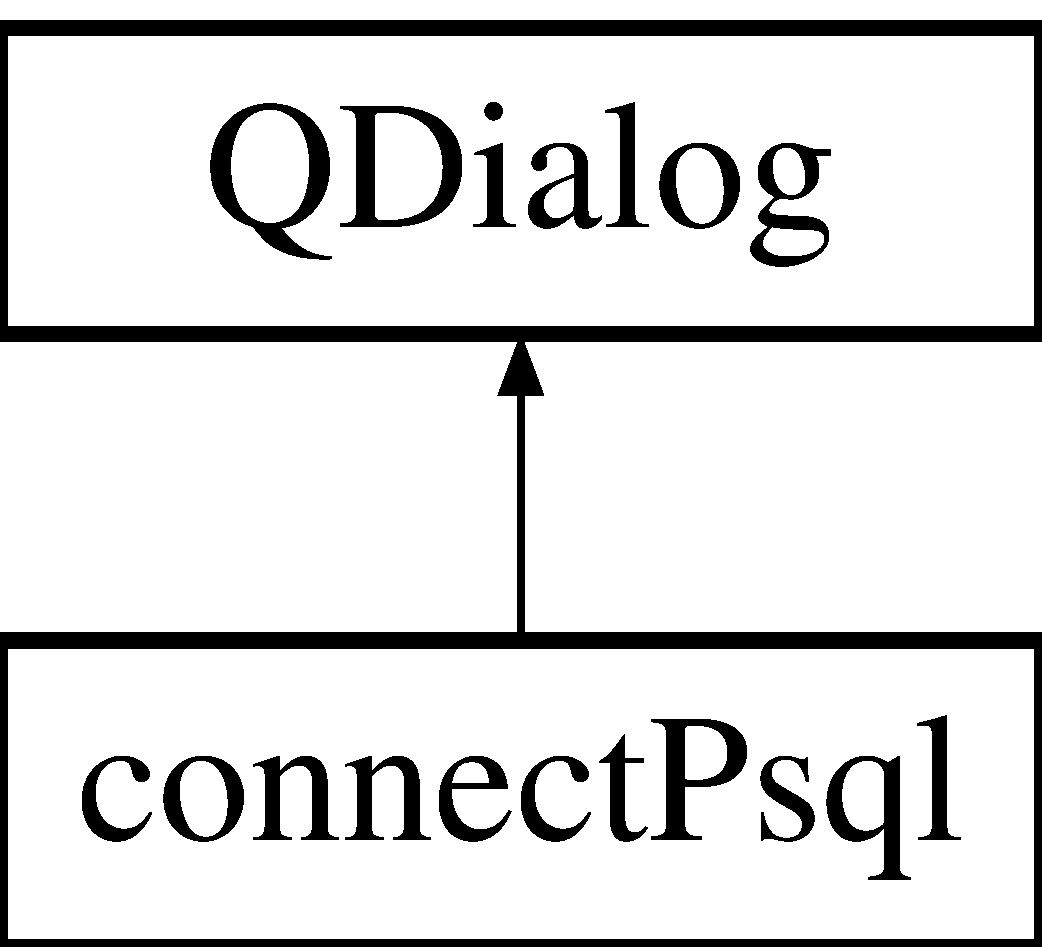
\includegraphics[height=2.000000cm]{classconnect_psql}
\end{center}
\end{figure}
\subsection*{Public Member Functions}
\begin{DoxyCompactItemize}
\item 
\hyperlink{classconnect_psql_aee2b55cd64f5b2fac084eda4e6db0075}{connect\+Psql} (Q\+String window\+Title, Q\+Widget $\ast$parent=0)
\begin{DoxyCompactList}\small\item\em \hyperlink{classconnect_psql}{connect\+Psql} Class constructor \end{DoxyCompactList}\end{DoxyCompactItemize}
\subsection*{Public Attributes}
\begin{DoxyCompactItemize}
\item 
\mbox{\Hypertarget{classconnect_psql_a5855dbe20b8e699563c0958462236bf2}\label{classconnect_psql_a5855dbe20b8e699563c0958462236bf2}} 
\hyperlink{classpsql}{psql} $\ast$ \hyperlink{classconnect_psql_a5855dbe20b8e699563c0958462236bf2}{p}
\begin{DoxyCompactList}\small\item\em p A Postgre\+S\+QL pointer \end{DoxyCompactList}\end{DoxyCompactItemize}


\subsection{Detailed Description}
The \hyperlink{classconnect_psql}{connect\+Psql} class. 

\subsection{Constructor \& Destructor Documentation}
\mbox{\Hypertarget{classconnect_psql_aee2b55cd64f5b2fac084eda4e6db0075}\label{classconnect_psql_aee2b55cd64f5b2fac084eda4e6db0075}} 
\index{connect\+Psql@{connect\+Psql}!connect\+Psql@{connect\+Psql}}
\index{connect\+Psql@{connect\+Psql}!connect\+Psql@{connect\+Psql}}
\subsubsection{\texorpdfstring{connect\+Psql()}{connectPsql()}}
{\footnotesize\ttfamily connect\+Psql\+::connect\+Psql (\begin{DoxyParamCaption}\item[{Q\+String}]{window\+Title,  }\item[{Q\+Widget $\ast$}]{parent = {\ttfamily 0} }\end{DoxyParamCaption})\hspace{0.3cm}{\ttfamily [explicit]}}



\hyperlink{classconnect_psql}{connect\+Psql} Class constructor 

\hyperlink{classconnect_psql_aee2b55cd64f5b2fac084eda4e6db0075}{connect\+Psql\+::connect\+Psql}


\begin{DoxyParams}{Parameters}
{\em parent} & \\
\hline
\end{DoxyParams}


The documentation for this class was generated from the following files\+:\begin{DoxyCompactItemize}
\item 
connectpsql.\+h\item 
connectpsql.\+cpp\end{DoxyCompactItemize}

\hypertarget{class_main_window}{}\section{Main\+Window Class Reference}
\label{class_main_window}\index{Main\+Window@{Main\+Window}}


The \mbox{\hyperlink{class_main_window}{Main\+Window}} class.  




{\ttfamily \#include $<$mainwindow.\+h$>$}

Inheritance diagram for Main\+Window\+:\begin{figure}[H]
\begin{center}
\leavevmode
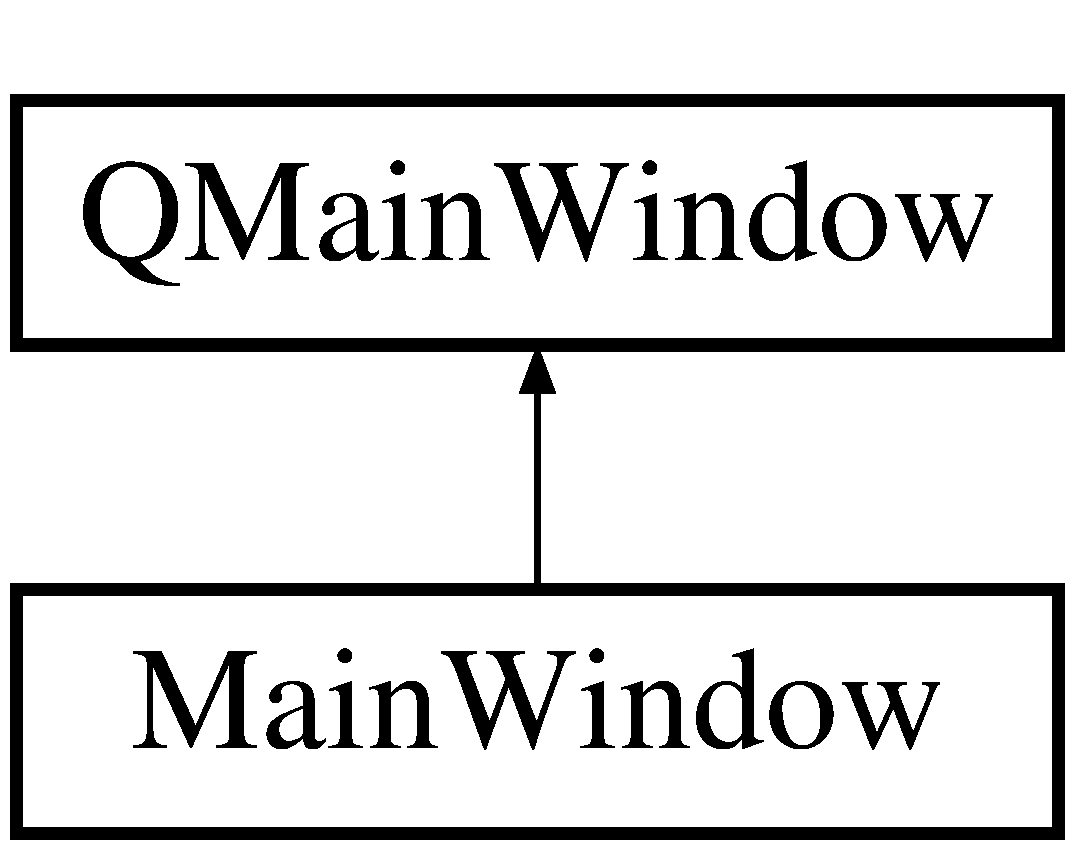
\includegraphics[height=2.000000cm]{class_main_window}
\end{center}
\end{figure}
\subsection*{Public Member Functions}
\begin{DoxyCompactItemize}
\item 
\mbox{\hyperlink{class_main_window_a8b244be8b7b7db1b08de2a2acb9409db}{Main\+Window}} (Q\+Widget $\ast$parent=0)
\begin{DoxyCompactList}\small\item\em \mbox{\hyperlink{class_main_window}{Main\+Window}} Class constructor. \end{DoxyCompactList}\end{DoxyCompactItemize}
\subsection*{Public Attributes}
\begin{DoxyCompactItemize}
\item 
\mbox{\Hypertarget{class_main_window_af6a0a464b2432a13ece4953de0e66441}\label{class_main_window_af6a0a464b2432a13ece4953de0e66441}} 
\mbox{\hyperlink{classconnect_psql}{connect\+Psql}} $\ast$ \mbox{\hyperlink{class_main_window_af6a0a464b2432a13ece4953de0e66441}{cp}}
\begin{DoxyCompactList}\small\item\em cp A pointer to the \mbox{\hyperlink{classconnect_psql}{connect\+Psql}} class \end{DoxyCompactList}\end{DoxyCompactItemize}


\subsection{Detailed Description}
The \mbox{\hyperlink{class_main_window}{Main\+Window}} class. 

\subsection{Constructor \& Destructor Documentation}
\mbox{\Hypertarget{class_main_window_a8b244be8b7b7db1b08de2a2acb9409db}\label{class_main_window_a8b244be8b7b7db1b08de2a2acb9409db}} 
\index{Main\+Window@{Main\+Window}!Main\+Window@{Main\+Window}}
\index{Main\+Window@{Main\+Window}!Main\+Window@{Main\+Window}}
\subsubsection{\texorpdfstring{Main\+Window()}{MainWindow()}}
{\footnotesize\ttfamily Main\+Window\+::\+Main\+Window (\begin{DoxyParamCaption}\item[{Q\+Widget $\ast$}]{parent = {\ttfamily 0} }\end{DoxyParamCaption})\hspace{0.3cm}{\ttfamily [explicit]}}



\mbox{\hyperlink{class_main_window}{Main\+Window}} Class constructor. 


\begin{DoxyParams}{Parameters}
{\em parent} & \\
\hline
\end{DoxyParams}


The documentation for this class was generated from the following files\+:\begin{DoxyCompactItemize}
\item 
mainwindow.\+h\item 
mainwindow.\+cpp\end{DoxyCompactItemize}

\hypertarget{class_new_city}{}\section{New\+City Class Reference}
\label{class_new_city}\index{NewCity@{NewCity}}


The \mbox{\hyperlink{class_new_city}{New\+City}} class.  




{\ttfamily \#include $<$newcity.\+h$>$}

Inheritance diagram for New\+City\+:\begin{figure}[H]
\begin{center}
\leavevmode
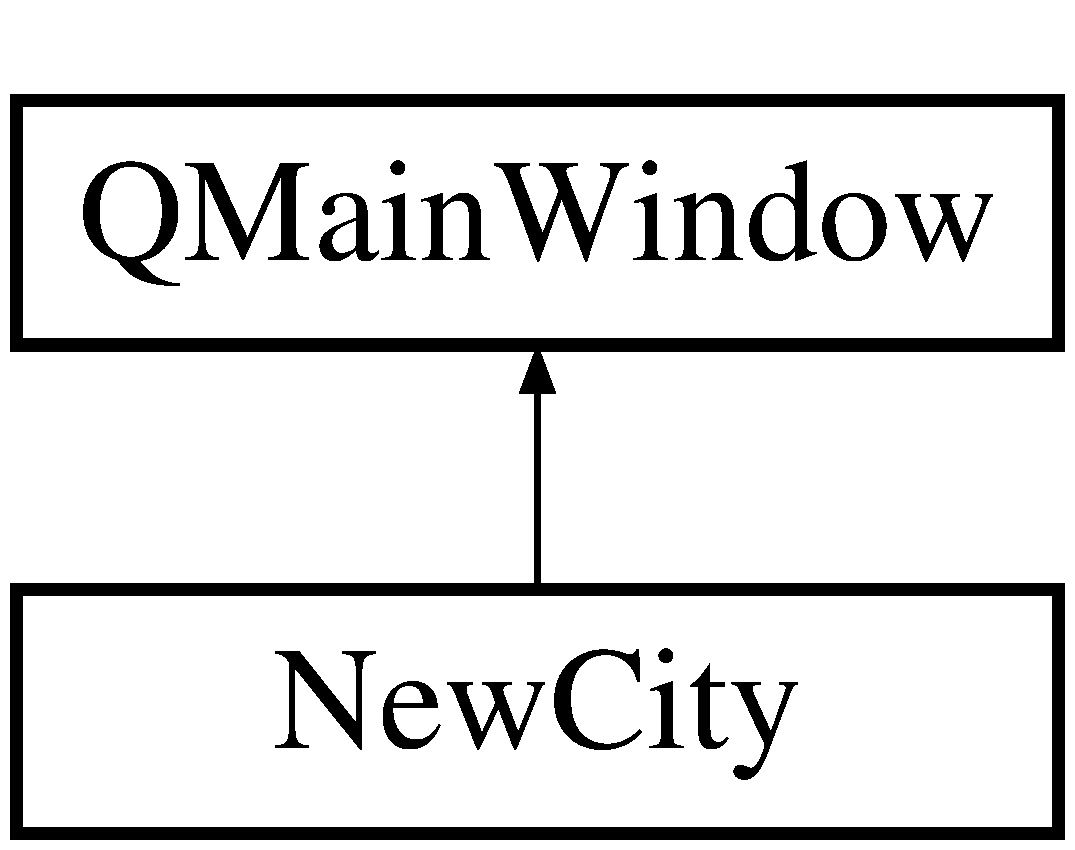
\includegraphics[height=2.000000cm]{class_new_city}
\end{center}
\end{figure}
\subsection*{Public Member Functions}
\begin{DoxyCompactItemize}
\item 
\mbox{\hyperlink{class_new_city_a8b626e1fe480368bc7c2f819c1de6a19}{New\+City}} (Q\+String window\+Title, \mbox{\hyperlink{classpsql}{psql}} $\ast$pg, Q\+Widget $\ast$parent=0)
\begin{DoxyCompactList}\small\item\em \mbox{\hyperlink{class_new_city}{New\+City}} The \mbox{\hyperlink{class_new_city}{New\+City}} class constructor. \end{DoxyCompactList}\item 
void \mbox{\hyperlink{class_new_city_a8a96f2c58640c96faf74e1f3bb956e4e}{set\+Country\+ID}} (int new\+Country\+ID)
\begin{DoxyCompactList}\small\item\em \mbox{\hyperlink{class_new_city_a8a96f2c58640c96faf74e1f3bb956e4e}{New\+City\+::set\+Country\+ID}} Sets a new country ID to be used when saving the new city to the database. \end{DoxyCompactList}\item 
int \mbox{\hyperlink{class_new_city_a743baefdc6604f1bf8da124056939b0c}{get\+Country\+ID}} ()
\begin{DoxyCompactList}\small\item\em \mbox{\hyperlink{class_new_city_a743baefdc6604f1bf8da124056939b0c}{New\+City\+::get\+Country\+ID}} Gets the chosen country ID. \end{DoxyCompactList}\item 
void \mbox{\hyperlink{class_new_city_afe093fcb1aa6623e896c52ea35ff0481}{set\+City\+Name}} (Q\+String name)
\begin{DoxyCompactList}\small\item\em \mbox{\hyperlink{class_new_city_afe093fcb1aa6623e896c52ea35ff0481}{New\+City\+::set\+City\+Name}} Sets the name of the new city. \end{DoxyCompactList}\item 
Q\+String \mbox{\hyperlink{class_new_city_a3be62538974fa100134d694546608877}{get\+City\+Name}} ()
\begin{DoxyCompactList}\small\item\em \mbox{\hyperlink{class_new_city_a3be62538974fa100134d694546608877}{New\+City\+::get\+City\+Name}} Gets the name of the new city. \end{DoxyCompactList}\end{DoxyCompactItemize}


\subsection{Detailed Description}
The \mbox{\hyperlink{class_new_city}{New\+City}} class. 

\subsection{Constructor \& Destructor Documentation}
\mbox{\Hypertarget{class_new_city_a8b626e1fe480368bc7c2f819c1de6a19}\label{class_new_city_a8b626e1fe480368bc7c2f819c1de6a19}} 
\index{NewCity@{NewCity}!NewCity@{NewCity}}
\index{NewCity@{NewCity}!NewCity@{NewCity}}
\subsubsection{\texorpdfstring{NewCity()}{NewCity()}}
{\footnotesize\ttfamily New\+City\+::\+New\+City (\begin{DoxyParamCaption}\item[{Q\+String}]{window\+Title,  }\item[{\mbox{\hyperlink{classpsql}{psql}} $\ast$}]{pg,  }\item[{Q\+Widget $\ast$}]{parent = {\ttfamily 0} }\end{DoxyParamCaption})\hspace{0.3cm}{\ttfamily [explicit]}}



\mbox{\hyperlink{class_new_city}{New\+City}} The \mbox{\hyperlink{class_new_city}{New\+City}} class constructor. 


\begin{DoxyParams}{Parameters}
{\em window\+Title} & The title to be used in message boxes, etc. \\
\hline
{\em pg} & Pointer to the Postgre\+S\+QL database \\
\hline
{\em parent} & \\
\hline
\end{DoxyParams}


\subsection{Member Function Documentation}
\mbox{\Hypertarget{class_new_city_a3be62538974fa100134d694546608877}\label{class_new_city_a3be62538974fa100134d694546608877}} 
\index{NewCity@{NewCity}!getCityName@{getCityName}}
\index{getCityName@{getCityName}!NewCity@{NewCity}}
\subsubsection{\texorpdfstring{getCityName()}{getCityName()}}
{\footnotesize\ttfamily Q\+String New\+City\+::get\+City\+Name (\begin{DoxyParamCaption}{ }\end{DoxyParamCaption})}



\mbox{\hyperlink{class_new_city_a3be62538974fa100134d694546608877}{New\+City\+::get\+City\+Name}} Gets the name of the new city. 

\begin{DoxyReturn}{Returns}
The name of the city to be saved in the database. 
\end{DoxyReturn}
\mbox{\Hypertarget{class_new_city_a743baefdc6604f1bf8da124056939b0c}\label{class_new_city_a743baefdc6604f1bf8da124056939b0c}} 
\index{NewCity@{NewCity}!getCountryID@{getCountryID}}
\index{getCountryID@{getCountryID}!NewCity@{NewCity}}
\subsubsection{\texorpdfstring{getCountryID()}{getCountryID()}}
{\footnotesize\ttfamily int New\+City\+::get\+Country\+ID (\begin{DoxyParamCaption}{ }\end{DoxyParamCaption})}



\mbox{\hyperlink{class_new_city_a743baefdc6604f1bf8da124056939b0c}{New\+City\+::get\+Country\+ID}} Gets the chosen country ID. 

\begin{DoxyReturn}{Returns}
The the country ID 
\end{DoxyReturn}
\mbox{\Hypertarget{class_new_city_afe093fcb1aa6623e896c52ea35ff0481}\label{class_new_city_afe093fcb1aa6623e896c52ea35ff0481}} 
\index{NewCity@{NewCity}!setCityName@{setCityName}}
\index{setCityName@{setCityName}!NewCity@{NewCity}}
\subsubsection{\texorpdfstring{setCityName()}{setCityName()}}
{\footnotesize\ttfamily void New\+City\+::set\+City\+Name (\begin{DoxyParamCaption}\item[{Q\+String}]{name }\end{DoxyParamCaption})}



\mbox{\hyperlink{class_new_city_afe093fcb1aa6623e896c52ea35ff0481}{New\+City\+::set\+City\+Name}} Sets the name of the new city. 


\begin{DoxyParams}{Parameters}
{\em name} & The new city name. \\
\hline
\end{DoxyParams}
\mbox{\Hypertarget{class_new_city_a8a96f2c58640c96faf74e1f3bb956e4e}\label{class_new_city_a8a96f2c58640c96faf74e1f3bb956e4e}} 
\index{NewCity@{NewCity}!setCountryID@{setCountryID}}
\index{setCountryID@{setCountryID}!NewCity@{NewCity}}
\subsubsection{\texorpdfstring{setCountryID()}{setCountryID()}}
{\footnotesize\ttfamily void New\+City\+::set\+Country\+ID (\begin{DoxyParamCaption}\item[{int}]{new\+Country\+ID }\end{DoxyParamCaption})}



\mbox{\hyperlink{class_new_city_a8a96f2c58640c96faf74e1f3bb956e4e}{New\+City\+::set\+Country\+ID}} Sets a new country ID to be used when saving the new city to the database. 


\begin{DoxyParams}{Parameters}
{\em new\+Country\+ID} & The ID of the country. \\
\hline
\end{DoxyParams}


The documentation for this class was generated from the following files\+:\begin{DoxyCompactItemize}
\item 
newcity.\+h\item 
\mbox{\hyperlink{newcity_8cpp}{newcity.\+cpp}}\end{DoxyCompactItemize}

\hypertarget{class_new_country}{}\section{New\+Country Class Reference}
\label{class_new_country}\index{New\+Country@{New\+Country}}
Inheritance diagram for New\+Country\+:\begin{figure}[H]
\begin{center}
\leavevmode
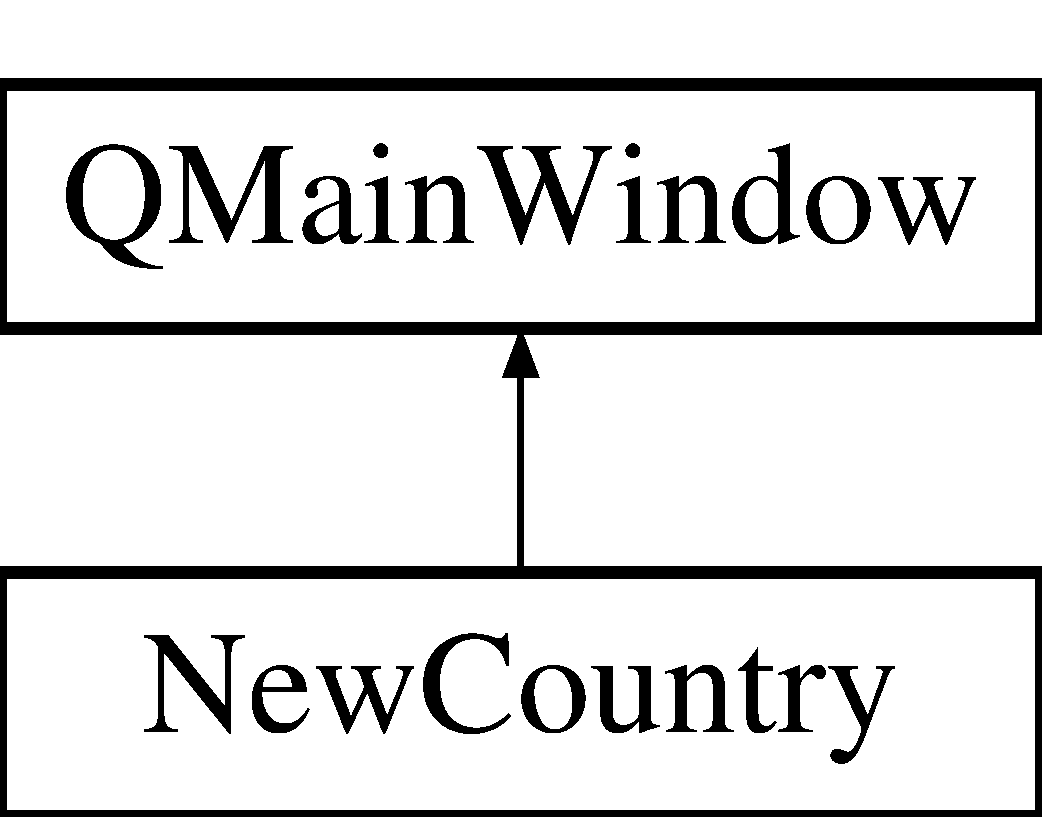
\includegraphics[height=2.000000cm]{class_new_country}
\end{center}
\end{figure}
\subsection*{Public Member Functions}
\begin{DoxyCompactItemize}
\item 
\hyperlink{class_new_country_a0ab1a95a2acd77e953f3a7aac8544880}{New\+Country} (Q\+String window\+Title, \hyperlink{classpsql}{psql} $\ast$pg, Q\+Widget $\ast$parent=0)
\begin{DoxyCompactList}\small\item\em \hyperlink{class_new_country_a0ab1a95a2acd77e953f3a7aac8544880}{New\+Country\+::\+New\+Country} \hyperlink{class_new_country}{New\+Country} class constructor. \end{DoxyCompactList}\item 
Q\+String \hyperlink{class_new_country_a5d28702b9788a1debf6817443d4a7355}{get\+Country} ()
\begin{DoxyCompactList}\small\item\em \hyperlink{class_new_country_a5d28702b9788a1debf6817443d4a7355}{New\+Country\+::get\+Country} Gets the current country name. \end{DoxyCompactList}\item 
void \hyperlink{class_new_country_af6fed97011d536e1a29db8112849e36b}{set\+Country} (Q\+String new\+Country)
\begin{DoxyCompactList}\small\item\em \hyperlink{class_new_country_af6fed97011d536e1a29db8112849e36b}{New\+Country\+::set\+Country} Sets the name of the country. \end{DoxyCompactList}\end{DoxyCompactItemize}


\subsection{Constructor \& Destructor Documentation}
\mbox{\Hypertarget{class_new_country_a0ab1a95a2acd77e953f3a7aac8544880}\label{class_new_country_a0ab1a95a2acd77e953f3a7aac8544880}} 
\index{New\+Country@{New\+Country}!New\+Country@{New\+Country}}
\index{New\+Country@{New\+Country}!New\+Country@{New\+Country}}
\subsubsection{\texorpdfstring{New\+Country()}{NewCountry()}}
{\footnotesize\ttfamily New\+Country\+::\+New\+Country (\begin{DoxyParamCaption}\item[{Q\+String}]{window\+Title,  }\item[{\hyperlink{classpsql}{psql} $\ast$}]{pg,  }\item[{Q\+Widget $\ast$}]{parent = {\ttfamily 0} }\end{DoxyParamCaption})\hspace{0.3cm}{\ttfamily [explicit]}}



\hyperlink{class_new_country_a0ab1a95a2acd77e953f3a7aac8544880}{New\+Country\+::\+New\+Country} \hyperlink{class_new_country}{New\+Country} class constructor. 


\begin{DoxyParams}{Parameters}
{\em window\+Title} & The title to be used with message boxes (Q\+Message\+Box) \\
\hline
{\em pg} & A pointer to the Postgre\+S\+QL database class \\
\hline
{\em parent} & \\
\hline
\end{DoxyParams}


\subsection{Member Function Documentation}
\mbox{\Hypertarget{class_new_country_a5d28702b9788a1debf6817443d4a7355}\label{class_new_country_a5d28702b9788a1debf6817443d4a7355}} 
\index{New\+Country@{New\+Country}!get\+Country@{get\+Country}}
\index{get\+Country@{get\+Country}!New\+Country@{New\+Country}}
\subsubsection{\texorpdfstring{get\+Country()}{getCountry()}}
{\footnotesize\ttfamily Q\+String New\+Country\+::get\+Country (\begin{DoxyParamCaption}{ }\end{DoxyParamCaption})}



\hyperlink{class_new_country_a5d28702b9788a1debf6817443d4a7355}{New\+Country\+::get\+Country} Gets the current country name. 

\begin{DoxyReturn}{Returns}
The name of the country 
\end{DoxyReturn}
\mbox{\Hypertarget{class_new_country_af6fed97011d536e1a29db8112849e36b}\label{class_new_country_af6fed97011d536e1a29db8112849e36b}} 
\index{New\+Country@{New\+Country}!set\+Country@{set\+Country}}
\index{set\+Country@{set\+Country}!New\+Country@{New\+Country}}
\subsubsection{\texorpdfstring{set\+Country()}{setCountry()}}
{\footnotesize\ttfamily void New\+Country\+::set\+Country (\begin{DoxyParamCaption}\item[{Q\+String}]{new\+Country }\end{DoxyParamCaption})}



\hyperlink{class_new_country_af6fed97011d536e1a29db8112849e36b}{New\+Country\+::set\+Country} Sets the name of the country. 


\begin{DoxyParams}{Parameters}
{\em new\+Country} & The new name of the country \\
\hline
\end{DoxyParams}


The documentation for this class was generated from the following files\+:\begin{DoxyCompactItemize}
\item 
newcountry.\+h\item 
newcountry.\+cpp\end{DoxyCompactItemize}

\hypertarget{class_new_job}{}\section{New\+Job Class Reference}
\label{class_new_job}\index{New\+Job@{New\+Job}}


The \hyperlink{class_new_job}{New\+Job} class.  




{\ttfamily \#include $<$newjob.\+h$>$}

Inheritance diagram for New\+Job\+:\begin{figure}[H]
\begin{center}
\leavevmode
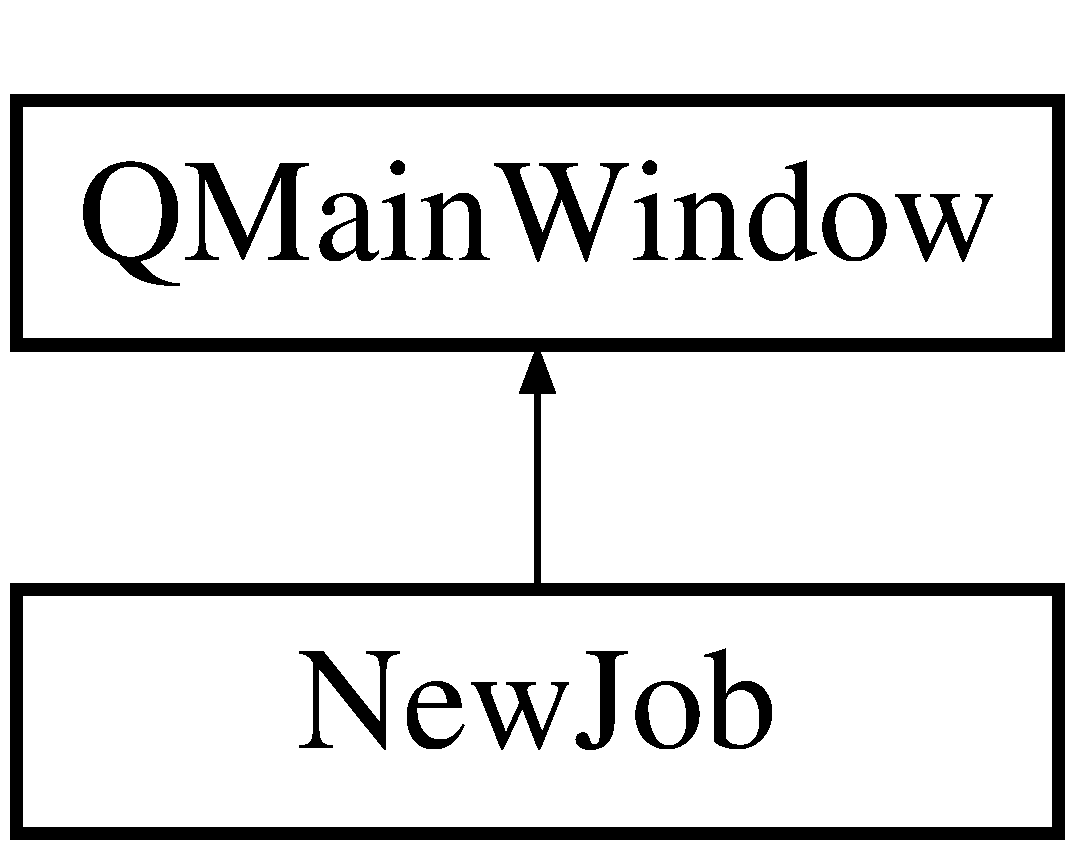
\includegraphics[height=2.000000cm]{class_new_job}
\end{center}
\end{figure}
\subsection*{Public Member Functions}
\begin{DoxyCompactItemize}
\item 
\hyperlink{class_new_job_a8a989ea2877d88189001ab4d9acf70cb}{New\+Job} (\hyperlink{classpsql}{psql} $\ast$pg, Q\+Widget $\ast$parent=0)
\begin{DoxyCompactList}\small\item\em \hyperlink{class_new_job}{New\+Job} The \hyperlink{class_new_job}{New\+Job} class constructor. \end{DoxyCompactList}\item 
void \hyperlink{class_new_job_ae8c2b576f2ea6f444776e6d944f0d767}{set\+Title} (Q\+String new\+Title)
\begin{DoxyCompactList}\small\item\em \hyperlink{class_new_job_ae8c2b576f2ea6f444776e6d944f0d767}{New\+Job\+::set\+Title}\+: Sets a new job title. \end{DoxyCompactList}\item 
void \hyperlink{class_new_job_ad9f522f4a6a45348ecc3ab1229b5eabb}{set\+Company} (Q\+String new\+Company)
\begin{DoxyCompactList}\small\item\em \hyperlink{class_new_job_ad9f522f4a6a45348ecc3ab1229b5eabb}{New\+Job\+::set\+Company}\+: Sets a new job company. \end{DoxyCompactList}\item 
void \hyperlink{class_new_job_a715852b239121af2b12ce36eded8faa0}{set\+City\+ID} (int new\+City\+ID)
\begin{DoxyCompactList}\small\item\em \hyperlink{class_new_job_a715852b239121af2b12ce36eded8faa0}{New\+Job\+::set\+City\+ID}\+: Sets the ID of the city in which the job is located. \end{DoxyCompactList}\item 
void \hyperlink{class_new_job_aa184d2046d0e60e82cd5840c40b99bed}{set\+Status\+ID} (int new\+Status\+ID)
\begin{DoxyCompactList}\small\item\em \hyperlink{class_new_job_aa184d2046d0e60e82cd5840c40b99bed}{New\+Job\+::set\+Status\+ID}\+: Sets the status ID of the job application. \end{DoxyCompactList}\item 
void \hyperlink{class_new_job_a0a1d9067e72f797ad3b1f01d44fedb0f}{set\+Date} (Q\+String new\+Date)
\begin{DoxyCompactList}\small\item\em \hyperlink{class_new_job_a0a1d9067e72f797ad3b1f01d44fedb0f}{New\+Job\+::set\+Date}\+: Sets the deadline for when the job application has to be sent. \end{DoxyCompactList}\item 
Q\+String \hyperlink{class_new_job_aa93c07712d80644b828994a01993c27c}{get\+Title} ()
\begin{DoxyCompactList}\small\item\em \hyperlink{class_new_job_aa93c07712d80644b828994a01993c27c}{New\+Job\+::get\+Title}\+: Gets the position title. \end{DoxyCompactList}\item 
Q\+String \hyperlink{class_new_job_ad4680ae9c009b90ce751c3c5fe60cdb5}{get\+Company} ()
\begin{DoxyCompactList}\small\item\em \hyperlink{class_new_job_ad4680ae9c009b90ce751c3c5fe60cdb5}{New\+Job\+::get\+Company}\+: Gets the name of the company. \end{DoxyCompactList}\item 
int \hyperlink{class_new_job_aed4a9a6fa7eab69062c1d36afd58cd75}{get\+City\+ID} ()
\begin{DoxyCompactList}\small\item\em \hyperlink{class_new_job_aed4a9a6fa7eab69062c1d36afd58cd75}{New\+Job\+::get\+City\+ID}\+: Gets the ID of the city where the job is located. \end{DoxyCompactList}\item 
int \hyperlink{class_new_job_aebbe015a22f5dbf60a34c33dd5c5a8e7}{get\+Status\+ID} ()
\begin{DoxyCompactList}\small\item\em \hyperlink{class_new_job_aebbe015a22f5dbf60a34c33dd5c5a8e7}{New\+Job\+::get\+Status\+ID}\+: Gets the current status ID of the job. \end{DoxyCompactList}\item 
Q\+String \hyperlink{class_new_job_abe92b6bce4e8e3485f59554a2cbad1bc}{get\+Date} ()
\begin{DoxyCompactList}\small\item\em \hyperlink{class_new_job_abe92b6bce4e8e3485f59554a2cbad1bc}{New\+Job\+::get\+Date}\+: Gets the job\textquotesingle{}s current application deadline. \end{DoxyCompactList}\item 
void \hyperlink{class_new_job_a84f6390f63ce01fb860b375f53f9c68d}{close\+Event} (Q\+Close\+Event $\ast$event) override
\begin{DoxyCompactList}\small\item\em close\+Event Code to be executed when the window closes \end{DoxyCompactList}\end{DoxyCompactItemize}


\subsection{Detailed Description}
The \hyperlink{class_new_job}{New\+Job} class. 

\subsection{Constructor \& Destructor Documentation}
\mbox{\Hypertarget{class_new_job_a8a989ea2877d88189001ab4d9acf70cb}\label{class_new_job_a8a989ea2877d88189001ab4d9acf70cb}} 
\index{New\+Job@{New\+Job}!New\+Job@{New\+Job}}
\index{New\+Job@{New\+Job}!New\+Job@{New\+Job}}
\subsubsection{\texorpdfstring{New\+Job()}{NewJob()}}
{\footnotesize\ttfamily New\+Job\+::\+New\+Job (\begin{DoxyParamCaption}\item[{\hyperlink{classpsql}{psql} $\ast$}]{pg,  }\item[{Q\+Widget $\ast$}]{parent = {\ttfamily 0} }\end{DoxyParamCaption})\hspace{0.3cm}{\ttfamily [explicit]}}



\hyperlink{class_new_job}{New\+Job} The \hyperlink{class_new_job}{New\+Job} class constructor. 


\begin{DoxyParams}{Parameters}
{\em pg} & A pointer to the Postgre\+S\+QL database. \\
\hline
{\em parent} & \\
\hline
\end{DoxyParams}


\subsection{Member Function Documentation}
\mbox{\Hypertarget{class_new_job_a84f6390f63ce01fb860b375f53f9c68d}\label{class_new_job_a84f6390f63ce01fb860b375f53f9c68d}} 
\index{New\+Job@{New\+Job}!close\+Event@{close\+Event}}
\index{close\+Event@{close\+Event}!New\+Job@{New\+Job}}
\subsubsection{\texorpdfstring{close\+Event()}{closeEvent()}}
{\footnotesize\ttfamily void New\+Job\+::close\+Event (\begin{DoxyParamCaption}\item[{Q\+Close\+Event $\ast$}]{event }\end{DoxyParamCaption})\hspace{0.3cm}{\ttfamily [override]}}



close\+Event Code to be executed when the window closes 


\begin{DoxyParams}{Parameters}
{\em event} & This pointer points to the Q\+Close\+Event class that contains functions to prvent the window from closing. \\
\hline
\end{DoxyParams}
\mbox{\Hypertarget{class_new_job_aed4a9a6fa7eab69062c1d36afd58cd75}\label{class_new_job_aed4a9a6fa7eab69062c1d36afd58cd75}} 
\index{New\+Job@{New\+Job}!get\+City\+ID@{get\+City\+ID}}
\index{get\+City\+ID@{get\+City\+ID}!New\+Job@{New\+Job}}
\subsubsection{\texorpdfstring{get\+City\+I\+D()}{getCityID()}}
{\footnotesize\ttfamily int New\+Job\+::get\+City\+ID (\begin{DoxyParamCaption}{ }\end{DoxyParamCaption})}



\hyperlink{class_new_job_aed4a9a6fa7eab69062c1d36afd58cd75}{New\+Job\+::get\+City\+ID}\+: Gets the ID of the city where the job is located. 

\begin{DoxyReturn}{Returns}
the ID of the city where the job is located. 
\end{DoxyReturn}
\mbox{\Hypertarget{class_new_job_ad4680ae9c009b90ce751c3c5fe60cdb5}\label{class_new_job_ad4680ae9c009b90ce751c3c5fe60cdb5}} 
\index{New\+Job@{New\+Job}!get\+Company@{get\+Company}}
\index{get\+Company@{get\+Company}!New\+Job@{New\+Job}}
\subsubsection{\texorpdfstring{get\+Company()}{getCompany()}}
{\footnotesize\ttfamily Q\+String New\+Job\+::get\+Company (\begin{DoxyParamCaption}{ }\end{DoxyParamCaption})}



\hyperlink{class_new_job_ad4680ae9c009b90ce751c3c5fe60cdb5}{New\+Job\+::get\+Company}\+: Gets the name of the company. 

\begin{DoxyReturn}{Returns}
The name of the company 
\end{DoxyReturn}
\mbox{\Hypertarget{class_new_job_abe92b6bce4e8e3485f59554a2cbad1bc}\label{class_new_job_abe92b6bce4e8e3485f59554a2cbad1bc}} 
\index{New\+Job@{New\+Job}!get\+Date@{get\+Date}}
\index{get\+Date@{get\+Date}!New\+Job@{New\+Job}}
\subsubsection{\texorpdfstring{get\+Date()}{getDate()}}
{\footnotesize\ttfamily Q\+String New\+Job\+::get\+Date (\begin{DoxyParamCaption}{ }\end{DoxyParamCaption})}



\hyperlink{class_new_job_abe92b6bce4e8e3485f59554a2cbad1bc}{New\+Job\+::get\+Date}\+: Gets the job\textquotesingle{}s current application deadline. 

\begin{DoxyReturn}{Returns}
The deadline of the job 
\end{DoxyReturn}
\mbox{\Hypertarget{class_new_job_aebbe015a22f5dbf60a34c33dd5c5a8e7}\label{class_new_job_aebbe015a22f5dbf60a34c33dd5c5a8e7}} 
\index{New\+Job@{New\+Job}!get\+Status\+ID@{get\+Status\+ID}}
\index{get\+Status\+ID@{get\+Status\+ID}!New\+Job@{New\+Job}}
\subsubsection{\texorpdfstring{get\+Status\+I\+D()}{getStatusID()}}
{\footnotesize\ttfamily int New\+Job\+::get\+Status\+ID (\begin{DoxyParamCaption}{ }\end{DoxyParamCaption})}



\hyperlink{class_new_job_aebbe015a22f5dbf60a34c33dd5c5a8e7}{New\+Job\+::get\+Status\+ID}\+: Gets the current status ID of the job. 

\begin{DoxyReturn}{Returns}
the ID of the job\textquotesingle{}s status 
\end{DoxyReturn}
\mbox{\Hypertarget{class_new_job_aa93c07712d80644b828994a01993c27c}\label{class_new_job_aa93c07712d80644b828994a01993c27c}} 
\index{New\+Job@{New\+Job}!get\+Title@{get\+Title}}
\index{get\+Title@{get\+Title}!New\+Job@{New\+Job}}
\subsubsection{\texorpdfstring{get\+Title()}{getTitle()}}
{\footnotesize\ttfamily Q\+String New\+Job\+::get\+Title (\begin{DoxyParamCaption}{ }\end{DoxyParamCaption})}



\hyperlink{class_new_job_aa93c07712d80644b828994a01993c27c}{New\+Job\+::get\+Title}\+: Gets the position title. 

\begin{DoxyReturn}{Returns}
The position title 
\end{DoxyReturn}
\mbox{\Hypertarget{class_new_job_a715852b239121af2b12ce36eded8faa0}\label{class_new_job_a715852b239121af2b12ce36eded8faa0}} 
\index{New\+Job@{New\+Job}!set\+City\+ID@{set\+City\+ID}}
\index{set\+City\+ID@{set\+City\+ID}!New\+Job@{New\+Job}}
\subsubsection{\texorpdfstring{set\+City\+I\+D()}{setCityID()}}
{\footnotesize\ttfamily void New\+Job\+::set\+City\+ID (\begin{DoxyParamCaption}\item[{int}]{new\+City\+ID }\end{DoxyParamCaption})}



\hyperlink{class_new_job_a715852b239121af2b12ce36eded8faa0}{New\+Job\+::set\+City\+ID}\+: Sets the ID of the city in which the job is located. 


\begin{DoxyParams}{Parameters}
{\em new\+City\+ID} & the ID of the city in which the job is located. \\
\hline
\end{DoxyParams}
\mbox{\Hypertarget{class_new_job_ad9f522f4a6a45348ecc3ab1229b5eabb}\label{class_new_job_ad9f522f4a6a45348ecc3ab1229b5eabb}} 
\index{New\+Job@{New\+Job}!set\+Company@{set\+Company}}
\index{set\+Company@{set\+Company}!New\+Job@{New\+Job}}
\subsubsection{\texorpdfstring{set\+Company()}{setCompany()}}
{\footnotesize\ttfamily void New\+Job\+::set\+Company (\begin{DoxyParamCaption}\item[{Q\+String}]{new\+Company }\end{DoxyParamCaption})}



\hyperlink{class_new_job_ad9f522f4a6a45348ecc3ab1229b5eabb}{New\+Job\+::set\+Company}\+: Sets a new job company. 


\begin{DoxyParams}{Parameters}
{\em new\+Company} & The new job company \\
\hline
\end{DoxyParams}
\mbox{\Hypertarget{class_new_job_a0a1d9067e72f797ad3b1f01d44fedb0f}\label{class_new_job_a0a1d9067e72f797ad3b1f01d44fedb0f}} 
\index{New\+Job@{New\+Job}!set\+Date@{set\+Date}}
\index{set\+Date@{set\+Date}!New\+Job@{New\+Job}}
\subsubsection{\texorpdfstring{set\+Date()}{setDate()}}
{\footnotesize\ttfamily void New\+Job\+::set\+Date (\begin{DoxyParamCaption}\item[{Q\+String}]{new\+Date }\end{DoxyParamCaption})}



\hyperlink{class_new_job_a0a1d9067e72f797ad3b1f01d44fedb0f}{New\+Job\+::set\+Date}\+: Sets the deadline for when the job application has to be sent. 


\begin{DoxyParams}{Parameters}
{\em new\+Date} & The deadline of the new job. \\
\hline
\end{DoxyParams}
\mbox{\Hypertarget{class_new_job_aa184d2046d0e60e82cd5840c40b99bed}\label{class_new_job_aa184d2046d0e60e82cd5840c40b99bed}} 
\index{New\+Job@{New\+Job}!set\+Status\+ID@{set\+Status\+ID}}
\index{set\+Status\+ID@{set\+Status\+ID}!New\+Job@{New\+Job}}
\subsubsection{\texorpdfstring{set\+Status\+I\+D()}{setStatusID()}}
{\footnotesize\ttfamily void New\+Job\+::set\+Status\+ID (\begin{DoxyParamCaption}\item[{int}]{new\+Status\+ID }\end{DoxyParamCaption})}



\hyperlink{class_new_job_aa184d2046d0e60e82cd5840c40b99bed}{New\+Job\+::set\+Status\+ID}\+: Sets the status ID of the job application. 


\begin{DoxyParams}{Parameters}
{\em new\+Status\+ID} & The new status ID of the job application \\
\hline
\end{DoxyParams}
\mbox{\Hypertarget{class_new_job_ae8c2b576f2ea6f444776e6d944f0d767}\label{class_new_job_ae8c2b576f2ea6f444776e6d944f0d767}} 
\index{New\+Job@{New\+Job}!set\+Title@{set\+Title}}
\index{set\+Title@{set\+Title}!New\+Job@{New\+Job}}
\subsubsection{\texorpdfstring{set\+Title()}{setTitle()}}
{\footnotesize\ttfamily void New\+Job\+::set\+Title (\begin{DoxyParamCaption}\item[{Q\+String}]{new\+Title }\end{DoxyParamCaption})}



\hyperlink{class_new_job_ae8c2b576f2ea6f444776e6d944f0d767}{New\+Job\+::set\+Title}\+: Sets a new job title. 


\begin{DoxyParams}{Parameters}
{\em new\+Title} & The new job title. \\
\hline
\end{DoxyParams}


The documentation for this class was generated from the following files\+:\begin{DoxyCompactItemize}
\item 
newjob.\+h\item 
newjob.\+cpp\end{DoxyCompactItemize}

\hypertarget{class_new_status}{}\section{New\+Status Class Reference}
\label{class_new_status}\index{New\+Status@{New\+Status}}


The \mbox{\hyperlink{class_new_status}{New\+Status}} class.  




{\ttfamily \#include $<$newstatus.\+h$>$}

Inheritance diagram for New\+Status\+:\begin{figure}[H]
\begin{center}
\leavevmode
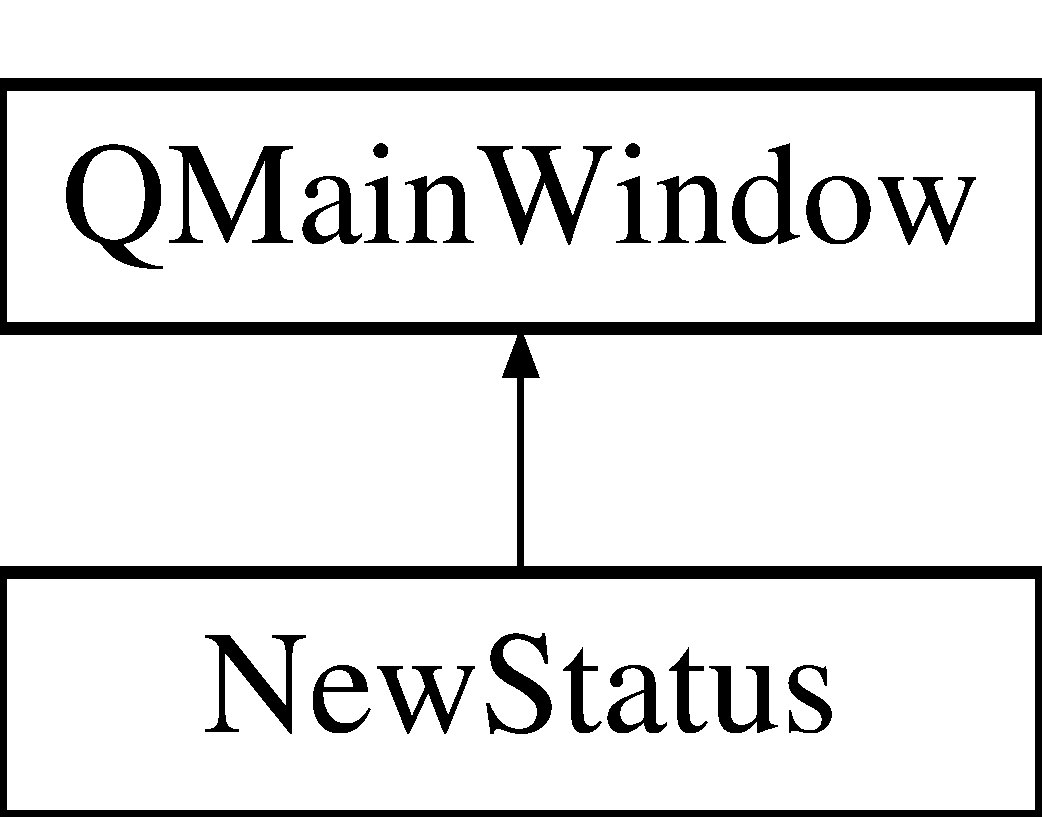
\includegraphics[height=2.000000cm]{class_new_status}
\end{center}
\end{figure}
\subsection*{Public Member Functions}
\begin{DoxyCompactItemize}
\item 
\mbox{\hyperlink{class_new_status_a5a09743191f617f006bc89e4b35984bf}{New\+Status}} (Q\+String window\+Title, \mbox{\hyperlink{classpsql}{psql}} $\ast$pg, Q\+Widget $\ast$parent=0)
\begin{DoxyCompactList}\small\item\em \mbox{\hyperlink{class_new_status}{New\+Status}} \mbox{\hyperlink{class_new_status}{New\+Status}} class constructor. \end{DoxyCompactList}\item 
void \mbox{\hyperlink{class_new_status_a861326c3b5c45040b933e4e65a4646e2}{set\+Status}} (Q\+String new\+Status)
\begin{DoxyCompactList}\small\item\em \mbox{\hyperlink{class_new_status_a861326c3b5c45040b933e4e65a4646e2}{New\+Status\+::set\+Status}} Sets the new status name. \end{DoxyCompactList}\item 
Q\+String \mbox{\hyperlink{class_new_status_a7ea744ad1645c5954000983d50947154}{get\+Status}} ()
\begin{DoxyCompactList}\small\item\em \mbox{\hyperlink{class_new_status_a7ea744ad1645c5954000983d50947154}{New\+Status\+::get\+Status}} Gets the current status name. \end{DoxyCompactList}\end{DoxyCompactItemize}


\subsection{Detailed Description}
The \mbox{\hyperlink{class_new_status}{New\+Status}} class. 

\subsection{Constructor \& Destructor Documentation}
\mbox{\Hypertarget{class_new_status_a5a09743191f617f006bc89e4b35984bf}\label{class_new_status_a5a09743191f617f006bc89e4b35984bf}} 
\index{New\+Status@{New\+Status}!New\+Status@{New\+Status}}
\index{New\+Status@{New\+Status}!New\+Status@{New\+Status}}
\subsubsection{\texorpdfstring{New\+Status()}{NewStatus()}}
{\footnotesize\ttfamily New\+Status\+::\+New\+Status (\begin{DoxyParamCaption}\item[{Q\+String}]{window\+Title,  }\item[{\mbox{\hyperlink{classpsql}{psql}} $\ast$}]{pg,  }\item[{Q\+Widget $\ast$}]{parent = {\ttfamily 0} }\end{DoxyParamCaption})\hspace{0.3cm}{\ttfamily [explicit]}}



\mbox{\hyperlink{class_new_status}{New\+Status}} \mbox{\hyperlink{class_new_status}{New\+Status}} class constructor. 


\begin{DoxyParams}{Parameters}
{\em window\+Title} & The title to be used with message boxes (Q\+Message\+Box) \\
\hline
{\em pg} & A pointer to the Postgre\+S\+QL database class \\
\hline
{\em parent} & \\
\hline
\end{DoxyParams}


\subsection{Member Function Documentation}
\mbox{\Hypertarget{class_new_status_a7ea744ad1645c5954000983d50947154}\label{class_new_status_a7ea744ad1645c5954000983d50947154}} 
\index{New\+Status@{New\+Status}!get\+Status@{get\+Status}}
\index{get\+Status@{get\+Status}!New\+Status@{New\+Status}}
\subsubsection{\texorpdfstring{get\+Status()}{getStatus()}}
{\footnotesize\ttfamily Q\+String New\+Status\+::get\+Status (\begin{DoxyParamCaption}{ }\end{DoxyParamCaption})}



\mbox{\hyperlink{class_new_status_a7ea744ad1645c5954000983d50947154}{New\+Status\+::get\+Status}} Gets the current status name. 

\begin{DoxyReturn}{Returns}
The status name to be returned. 
\end{DoxyReturn}
\mbox{\Hypertarget{class_new_status_a861326c3b5c45040b933e4e65a4646e2}\label{class_new_status_a861326c3b5c45040b933e4e65a4646e2}} 
\index{New\+Status@{New\+Status}!set\+Status@{set\+Status}}
\index{set\+Status@{set\+Status}!New\+Status@{New\+Status}}
\subsubsection{\texorpdfstring{set\+Status()}{setStatus()}}
{\footnotesize\ttfamily void New\+Status\+::set\+Status (\begin{DoxyParamCaption}\item[{Q\+String}]{new\+Status }\end{DoxyParamCaption})}



\mbox{\hyperlink{class_new_status_a861326c3b5c45040b933e4e65a4646e2}{New\+Status\+::set\+Status}} Sets the new status name. 


\begin{DoxyParams}{Parameters}
{\em new\+Status} & the name of the new status \\
\hline
\end{DoxyParams}


The documentation for this class was generated from the following files\+:\begin{DoxyCompactItemize}
\item 
newstatus.\+h\item 
newstatus.\+cpp\end{DoxyCompactItemize}

\hypertarget{classpsql}{}\section{psql Class Reference}
\label{classpsql}\index{psql@{psql}}


The psql class.  




{\ttfamily \#include $<$psql.\+h$>$}

\subsection*{Public Member Functions}
\begin{DoxyCompactItemize}
\item 
\mbox{\Hypertarget{classpsql_aaff5fe0931dce097850982e44e6361af}\label{classpsql_aaff5fe0931dce097850982e44e6361af}} 
{\bfseries psql} (Q\+String window\+Title)
\item 
Q\+String \hyperlink{classpsql_aecc9fd93dc5ca0c4f4a63d445a36d166}{get\+Username} ()
\begin{DoxyCompactList}\small\item\em \hyperlink{classpsql_aecc9fd93dc5ca0c4f4a63d445a36d166}{psql\+::get\+Username}\+: Gets the username \end{DoxyCompactList}\item 
Q\+String \hyperlink{classpsql_a817e5a88f877cac6f843c1e743aec096}{get\+Password} ()
\begin{DoxyCompactList}\small\item\em \hyperlink{classpsql_a817e5a88f877cac6f843c1e743aec096}{psql\+::get\+Password}\+: Gets the user password \end{DoxyCompactList}\item 
Q\+String \hyperlink{classpsql_a95d06ee661db0b9cf72605b983b04613}{get\+Host} ()
\begin{DoxyCompactList}\small\item\em \hyperlink{classpsql_a95d06ee661db0b9cf72605b983b04613}{psql\+::get\+Host}\+: Gets the IP address of the host \end{DoxyCompactList}\item 
\mbox{\Hypertarget{classpsql_a3aefa56fba453cffe18c3ae9d94af092}\label{classpsql_a3aefa56fba453cffe18c3ae9d94af092}} 
int {\bfseries get\+Rows} (string query)
\item 
void \hyperlink{classpsql_a96b3b9483f1a642c026d4b5cf505eb75}{set\+Host} (Q\+String new\+Host)
\begin{DoxyCompactList}\small\item\em \hyperlink{classpsql_a96b3b9483f1a642c026d4b5cf505eb75}{psql\+::set\+Host}\+: Sets the IP address of the new host \end{DoxyCompactList}\item 
void \hyperlink{classpsql_a6c29350037550b7e5a5bb8f439c405f3}{set\+Password} (Q\+String new\+Password)
\begin{DoxyCompactList}\small\item\em \hyperlink{classpsql_a6c29350037550b7e5a5bb8f439c405f3}{psql\+::set\+Password}\+: Sets the new password \end{DoxyCompactList}\item 
void \hyperlink{classpsql_a1488a9e4909abd172651b7be240342cb}{set\+Username} (Q\+String new\+User)
\begin{DoxyCompactList}\small\item\em \hyperlink{classpsql_a1488a9e4909abd172651b7be240342cb}{psql\+::set\+Username}\+: Sets the new username \end{DoxyCompactList}\item 
bool \hyperlink{classpsql_ada485c933df77453629e3821ab19fa4c}{connect\+Database} ()
\begin{DoxyCompactList}\small\item\em \hyperlink{classpsql_ada485c933df77453629e3821ab19fa4c}{psql\+::connect\+Database} Connects to the Postgre\+S\+QL database. \end{DoxyCompactList}\item 
bool \hyperlink{classpsql_a4073d4f70f2ae6211ba0328c2008407c}{insert\+Application} (Q\+String title, Q\+String company, int city\+ID, int status\+ID, Q\+String date)
\begin{DoxyCompactList}\small\item\em \hyperlink{classpsql_a4073d4f70f2ae6211ba0328c2008407c}{psql\+::insert\+Application} Inserts a new job application to the database. \end{DoxyCompactList}\item 
bool \hyperlink{classpsql_a767b85014d9df3eac148730f18888d6d}{insert\+City} (Q\+String city\+Name, int country\+ID)
\begin{DoxyCompactList}\small\item\em \hyperlink{classpsql_a767b85014d9df3eac148730f18888d6d}{psql\+::insert\+City} Inserts a new city to the database \end{DoxyCompactList}\item 
bool \hyperlink{classpsql_ab3b5934ce3fbc4be1730d990d4142893}{insert\+Country} (Q\+String country\+Name)
\begin{DoxyCompactList}\small\item\em \hyperlink{classpsql_ab3b5934ce3fbc4be1730d990d4142893}{psql\+::insert\+Country} Inserts a new country into the database \end{DoxyCompactList}\item 
bool \hyperlink{classpsql_a601ee0bdc9430b1d674a857f7c94b767}{insert\+Status} (Q\+String status\+Name)
\begin{DoxyCompactList}\small\item\em \hyperlink{classpsql_a601ee0bdc9430b1d674a857f7c94b767}{psql\+::insert\+Status} Inserts a new status to the database. \end{DoxyCompactList}\item 
bool \hyperlink{classpsql_a9a9c4c858ae22eac8a9a4572b16500f5}{update\+Application} (Q\+String title, Q\+String company, int city\+ID, int status\+ID, Q\+String date, int id)
\begin{DoxyCompactList}\small\item\em \hyperlink{classpsql_a9a9c4c858ae22eac8a9a4572b16500f5}{psql\+::update\+Application}\+: Updates the current job application \end{DoxyCompactList}\item 
bool \hyperlink{classpsql_a6adf2ba381783e520c03fe5324dcb010}{update\+City} (Q\+String city\+Name, int country\+ID, int id)
\begin{DoxyCompactList}\small\item\em \hyperlink{classpsql_a6adf2ba381783e520c03fe5324dcb010}{psql\+::update\+City} Updates information of an existing city. \end{DoxyCompactList}\item 
bool \hyperlink{classpsql_ae662278c5fb8ff3471ee1442e69482e2}{update\+Country} (Q\+String country\+Name, int country\+ID)
\begin{DoxyCompactList}\small\item\em \hyperlink{classpsql_ae662278c5fb8ff3471ee1442e69482e2}{psql\+::update\+Country} Updates an existing country. \end{DoxyCompactList}\item 
bool \hyperlink{classpsql_a620364c99c98e20720908deb045536a0}{update\+Status} (Q\+String statusname, int status\+ID)
\begin{DoxyCompactList}\small\item\em \hyperlink{classpsql_a620364c99c98e20720908deb045536a0}{psql\+::update\+Status} Updates an existing status. \end{DoxyCompactList}\item 
bool \hyperlink{classpsql_a999ee8e2d813892411ef502ebc055a79}{delete\+Application} (int application\+ID)
\begin{DoxyCompactList}\small\item\em \hyperlink{classpsql_a999ee8e2d813892411ef502ebc055a79}{psql\+::delete\+Application} Removes an application from the database. \end{DoxyCompactList}\item 
bool \hyperlink{classpsql_aaffd42b26b635d9881daaf5fbf4fd62f}{delete\+City} (int city\+ID)
\begin{DoxyCompactList}\small\item\em \hyperlink{classpsql_aaffd42b26b635d9881daaf5fbf4fd62f}{psql\+::delete\+City} Deletes an existing city from the database. \end{DoxyCompactList}\item 
bool \hyperlink{classpsql_a914bf8701fbed4ff80edcd0d09c7c3fd}{delete\+Country} (int country\+ID)
\begin{DoxyCompactList}\small\item\em \hyperlink{classpsql_a914bf8701fbed4ff80edcd0d09c7c3fd}{psql\+::delete\+Country} Deletes an existing country from the database. \end{DoxyCompactList}\item 
bool \hyperlink{classpsql_a26fc592cfb9f484e1bee62af527f2b95}{delete\+Status} (int status\+ID)
\begin{DoxyCompactList}\small\item\em \hyperlink{classpsql_a26fc592cfb9f484e1bee62af527f2b95}{psql\+::delete\+Status} Deletes an existing status from the database. \end{DoxyCompactList}\item 
Q\+String \hyperlink{classpsql_a5f51e254b67ff932f287df2184ccc043}{get\+Error} ()
\begin{DoxyCompactList}\small\item\em \hyperlink{classpsql_a5f51e254b67ff932f287df2184ccc043}{psql\+::get\+Error} If an operation goes wrong, this method can be used to get the returned error message. \end{DoxyCompactList}\item 
void \hyperlink{classpsql_a9a0d5ba32aabe6018a36fb0bc185445b}{set\+Error} (Q\+String msg)
\begin{DoxyCompactList}\small\item\em \hyperlink{classpsql_a9a0d5ba32aabe6018a36fb0bc185445b}{psql\+::set\+Error} If an operation goes wrong, this method saves the contents of the error message. \end{DoxyCompactList}\item 
\mbox{\Hypertarget{classpsql_a13f28a96fa9f79076ecae7d86280008f}\label{classpsql_a13f28a96fa9f79076ecae7d86280008f}} 
int {\bfseries get\+Application\+ID} (Q\+String qry)
\item 
int \hyperlink{classpsql_af3462a12dc106e0ca8df4fa8fcf28436}{get\+City\+ID} (int application\+ID)
\begin{DoxyCompactList}\small\item\em \hyperlink{classpsql_af3462a12dc106e0ca8df4fa8fcf28436}{psql\+::get\+City\+ID} Gets the city ID of the application based on the application ID prvoided by the user. \end{DoxyCompactList}\item 
int \hyperlink{classpsql_a81d02dc0350ba11d90257914078ba432}{get\+Country\+ID} (int city\+ID)
\begin{DoxyCompactList}\small\item\em \hyperlink{classpsql_a81d02dc0350ba11d90257914078ba432}{psql\+::get\+Country\+ID} Get the country ID of table sted based on given stedid. \end{DoxyCompactList}\item 
int \hyperlink{classpsql_a9c02c92c09cb60c35d24375673b7df06}{get\+Status\+ID} (int application\+ID)
\begin{DoxyCompactList}\small\item\em \hyperlink{classpsql_a9c02c92c09cb60c35d24375673b7df06}{psql\+::get\+Status\+ID} Returns the status ID of the application based on the application ID provided by the user. \end{DoxyCompactList}\item 
Q\+List$<$ int $>$ \hyperlink{classpsql_a9a3082a159c962dfcd84e23930f5619b}{fill\+List} (const char $\ast$sql\+Sporring)
\begin{DoxyCompactList}\small\item\em \hyperlink{classpsql_a9a3082a159c962dfcd84e23930f5619b}{psql\+::fill\+List} \char`\"{}\+Fills\char`\"{} a Q\+List with integers based on the results of an S\+QL query. \end{DoxyCompactList}\item 
Q\+List$<$ int $>$ \hyperlink{classpsql_ae262aec447273444deeda34113361e21}{get\+Specific\+Application\+I\+Ds} (string job\+Title, string company\+Name, string city\+Name, string status, string deadline)
\begin{DoxyCompactList}\small\item\em \hyperlink{classpsql_ae262aec447273444deeda34113361e21}{psql\+::get\+Specific\+Application\+I\+Ds} Builds a list of application I\+Ds based on search criteria. \end{DoxyCompactList}\item 
Q\+List$<$ Q\+String $>$ \hyperlink{classpsql_a62b208d687607bd78a6502444cecced8}{get\+Specific\+Job\+Names} (string job\+Title, string company\+Name, string city\+Name, string status, string deadline)
\begin{DoxyCompactList}\small\item\em \hyperlink{classpsql_a62b208d687607bd78a6502444cecced8}{psql\+::get\+Specific\+Job\+Names} Builds list of job titles based on search criteria. \end{DoxyCompactList}\item 
Q\+List$<$ Q\+String $>$ \hyperlink{classpsql_a47a1c719a9014f94706fdce665fdf21c}{get\+Specific\+Company\+Names} (string job\+Title, string company\+Name, string city\+Name, string status, string deadline)
\begin{DoxyCompactList}\small\item\em \hyperlink{classpsql_a47a1c719a9014f94706fdce665fdf21c}{psql\+::get\+Specific\+Company\+Names} Builds a list with name of job company/companies based on search criteria. \end{DoxyCompactList}\item 
Q\+List$<$ Q\+String $>$ \hyperlink{classpsql_ae337317b29abd16f3a52467d978b04ea}{get\+Specific\+City\+Names} (string job\+Title, string company\+Name, string city\+Name, string status, string deadline)
\begin{DoxyCompactList}\small\item\em \hyperlink{classpsql_ae337317b29abd16f3a52467d978b04ea}{psql\+::get\+Specific\+City\+Names} Builds a list of city names in one or more applications based on search criteria. \end{DoxyCompactList}\item 
Q\+List$<$ Q\+String $>$ \hyperlink{classpsql_a7635c79a1991c8271c813dbf02f7d123}{get\+Specific\+Statuses} (string job\+Title, string company\+Name, string city\+Name, string status, string deadline)
\begin{DoxyCompactList}\small\item\em \hyperlink{classpsql_a7635c79a1991c8271c813dbf02f7d123}{psql\+::get\+Specific\+Statuses} Builds a list of statuses based on the search criteria. \end{DoxyCompactList}\item 
Q\+List$<$ Q\+String $>$ \hyperlink{classpsql_a880551e9e539e52143a35dee2b07bff6}{get\+Specific\+Deadlines} (string job\+Title, string company\+Name, string city\+Name, string status, string deadline)
\begin{DoxyCompactList}\small\item\em \hyperlink{classpsql_a880551e9e539e52143a35dee2b07bff6}{psql\+::get\+Specific\+Deadlines} Builds a list of application deadlines based on search criteria \end{DoxyCompactList}\item 
Q\+List$<$ Q\+String $>$ \hyperlink{classpsql_a42ee0cf90055ba6a7a6f564cf04d8bb8}{get\+City\+Names} ()
\begin{DoxyCompactList}\small\item\em \hyperlink{classpsql_a42ee0cf90055ba6a7a6f564cf04d8bb8}{psql\+::get\+City\+Names} Builds a list of strings that cointain name of all cities in the database. \end{DoxyCompactList}\item 
Q\+List$<$ Q\+String $>$ \hyperlink{classpsql_a14854d28aabc7e658aea87a7b8b52e5c}{get\+Statuses} ()
\begin{DoxyCompactList}\small\item\em \hyperlink{classpsql_a14854d28aabc7e658aea87a7b8b52e5c}{psql\+::get\+Statuses} Builds a list of all statuses registered in the database. \end{DoxyCompactList}\item 
Q\+String \hyperlink{classpsql_a7acc18034ef60c8a1e69b0e1a15d8ab2}{get\+City\+Name} (int city\+Number)
\begin{DoxyCompactList}\small\item\em \hyperlink{classpsql_a7acc18034ef60c8a1e69b0e1a15d8ab2}{psql\+::get\+City\+Name} Gets the name of the city based on the city number. \end{DoxyCompactList}\item 
Q\+String \hyperlink{classpsql_a09745cd03f09ffb2dacacaab4281915f}{get\+Company} (int application\+ID)
\begin{DoxyCompactList}\small\item\em \hyperlink{classpsql_a09745cd03f09ffb2dacacaab4281915f}{psql\+::get\+Company} Gets the company name based on the application ID provided by the user. \end{DoxyCompactList}\item 
Q\+String \hyperlink{classpsql_a5724e9992e6a5c98524ab73b98f4202d}{get\+Country\+Name} (int country\+ID)
\begin{DoxyCompactList}\small\item\em \hyperlink{classpsql_a5724e9992e6a5c98524ab73b98f4202d}{psql\+::get\+Country\+Name} Gets the name of a country based on its ID. \end{DoxyCompactList}\item 
Q\+String \hyperlink{classpsql_a561f96bfe7e9d092077712dd6b186af8}{get\+Date} (int application\+ID)
\begin{DoxyCompactList}\small\item\em \hyperlink{classpsql_a561f96bfe7e9d092077712dd6b186af8}{psql\+::get\+Date} Gets the application deadline based on the application ID provided by the user. \end{DoxyCompactList}\item 
Q\+String \hyperlink{classpsql_a5c2a64419a68a258071fd1f9a37c7c09}{get\+Status\+Name} (int s)
\begin{DoxyCompactList}\small\item\em \hyperlink{classpsql_a5c2a64419a68a258071fd1f9a37c7c09}{psql\+::get\+Status\+Name} Returns the current status name \end{DoxyCompactList}\item 
Q\+String \hyperlink{classpsql_ada9e3be3e0866011edf53e30ec510afc}{get\+Title} (int application\+ID)
\begin{DoxyCompactList}\small\item\em \hyperlink{classpsql_ada9e3be3e0866011edf53e30ec510afc}{psql\+::get\+Title} Returns the application title based on the ID provided by the user \end{DoxyCompactList}\end{DoxyCompactItemize}


\subsection{Detailed Description}
The psql class. 

\subsection{Member Function Documentation}
\mbox{\Hypertarget{classpsql_ada485c933df77453629e3821ab19fa4c}\label{classpsql_ada485c933df77453629e3821ab19fa4c}} 
\index{psql@{psql}!connect\+Database@{connect\+Database}}
\index{connect\+Database@{connect\+Database}!psql@{psql}}
\subsubsection{\texorpdfstring{connect\+Database()}{connectDatabase()}}
{\footnotesize\ttfamily bool psql\+::connect\+Database (\begin{DoxyParamCaption}{ }\end{DoxyParamCaption})}



\hyperlink{classpsql_ada485c933df77453629e3821ab19fa4c}{psql\+::connect\+Database} Connects to the Postgre\+S\+QL database. 

\begin{DoxyReturn}{Returns}
True on successful connection and false on failure. 
\end{DoxyReturn}
\mbox{\Hypertarget{classpsql_a999ee8e2d813892411ef502ebc055a79}\label{classpsql_a999ee8e2d813892411ef502ebc055a79}} 
\index{psql@{psql}!delete\+Application@{delete\+Application}}
\index{delete\+Application@{delete\+Application}!psql@{psql}}
\subsubsection{\texorpdfstring{delete\+Application()}{deleteApplication()}}
{\footnotesize\ttfamily bool psql\+::delete\+Application (\begin{DoxyParamCaption}\item[{int}]{application\+ID }\end{DoxyParamCaption})}



\hyperlink{classpsql_a999ee8e2d813892411ef502ebc055a79}{psql\+::delete\+Application} Removes an application from the database. 


\begin{DoxyParams}{Parameters}
{\em application\+ID} & The ID of the application to be removed. \\
\hline
\end{DoxyParams}
\begin{DoxyReturn}{Returns}
True on successful removal and false otherwise. 
\end{DoxyReturn}
\mbox{\Hypertarget{classpsql_aaffd42b26b635d9881daaf5fbf4fd62f}\label{classpsql_aaffd42b26b635d9881daaf5fbf4fd62f}} 
\index{psql@{psql}!delete\+City@{delete\+City}}
\index{delete\+City@{delete\+City}!psql@{psql}}
\subsubsection{\texorpdfstring{delete\+City()}{deleteCity()}}
{\footnotesize\ttfamily bool psql\+::delete\+City (\begin{DoxyParamCaption}\item[{int}]{city\+ID }\end{DoxyParamCaption})}



\hyperlink{classpsql_aaffd42b26b635d9881daaf5fbf4fd62f}{psql\+::delete\+City} Deletes an existing city from the database. 


\begin{DoxyParams}{Parameters}
{\em city\+ID} & The unique identification number of the city to be removed. \\
\hline
\end{DoxyParams}
\begin{DoxyReturn}{Returns}
True on successful removal and false otherwise. 
\end{DoxyReturn}
\mbox{\Hypertarget{classpsql_a914bf8701fbed4ff80edcd0d09c7c3fd}\label{classpsql_a914bf8701fbed4ff80edcd0d09c7c3fd}} 
\index{psql@{psql}!delete\+Country@{delete\+Country}}
\index{delete\+Country@{delete\+Country}!psql@{psql}}
\subsubsection{\texorpdfstring{delete\+Country()}{deleteCountry()}}
{\footnotesize\ttfamily bool psql\+::delete\+Country (\begin{DoxyParamCaption}\item[{int}]{country\+ID }\end{DoxyParamCaption})}



\hyperlink{classpsql_a914bf8701fbed4ff80edcd0d09c7c3fd}{psql\+::delete\+Country} Deletes an existing country from the database. 


\begin{DoxyParams}{Parameters}
{\em country\+ID} & The unique number of the country in question. \\
\hline
\end{DoxyParams}
\begin{DoxyReturn}{Returns}
True on successful removal and false otherwise. 
\end{DoxyReturn}
\mbox{\Hypertarget{classpsql_a26fc592cfb9f484e1bee62af527f2b95}\label{classpsql_a26fc592cfb9f484e1bee62af527f2b95}} 
\index{psql@{psql}!delete\+Status@{delete\+Status}}
\index{delete\+Status@{delete\+Status}!psql@{psql}}
\subsubsection{\texorpdfstring{delete\+Status()}{deleteStatus()}}
{\footnotesize\ttfamily bool psql\+::delete\+Status (\begin{DoxyParamCaption}\item[{int}]{status\+ID }\end{DoxyParamCaption})}



\hyperlink{classpsql_a26fc592cfb9f484e1bee62af527f2b95}{psql\+::delete\+Status} Deletes an existing status from the database. 


\begin{DoxyParams}{Parameters}
{\em status\+ID} & The identification number of the status to be deleted. \\
\hline
\end{DoxyParams}
\begin{DoxyReturn}{Returns}
True on successful removal and false otherwise. 
\end{DoxyReturn}
\mbox{\Hypertarget{classpsql_a9a3082a159c962dfcd84e23930f5619b}\label{classpsql_a9a3082a159c962dfcd84e23930f5619b}} 
\index{psql@{psql}!fill\+List@{fill\+List}}
\index{fill\+List@{fill\+List}!psql@{psql}}
\subsubsection{\texorpdfstring{fill\+List()}{fillList()}}
{\footnotesize\ttfamily Q\+List$<$ int $>$ psql\+::fill\+List (\begin{DoxyParamCaption}\item[{const char $\ast$}]{sql\+Sporring }\end{DoxyParamCaption})}



\hyperlink{classpsql_a9a3082a159c962dfcd84e23930f5619b}{psql\+::fill\+List} \char`\"{}\+Fills\char`\"{} a Q\+List with integers based on the results of an S\+QL query. 


\begin{DoxyParams}{Parameters}
{\em sql\+Sporring} & The S\+QL query to be executed. \\
\hline
\end{DoxyParams}
\begin{DoxyReturn}{Returns}

\end{DoxyReturn}
\mbox{\Hypertarget{classpsql_af3462a12dc106e0ca8df4fa8fcf28436}\label{classpsql_af3462a12dc106e0ca8df4fa8fcf28436}} 
\index{psql@{psql}!get\+City\+ID@{get\+City\+ID}}
\index{get\+City\+ID@{get\+City\+ID}!psql@{psql}}
\subsubsection{\texorpdfstring{get\+City\+I\+D()}{getCityID()}}
{\footnotesize\ttfamily int psql\+::get\+City\+ID (\begin{DoxyParamCaption}\item[{int}]{application\+ID }\end{DoxyParamCaption})}



\hyperlink{classpsql_af3462a12dc106e0ca8df4fa8fcf28436}{psql\+::get\+City\+ID} Gets the city ID of the application based on the application ID prvoided by the user. 


\begin{DoxyParams}{Parameters}
{\em application\+ID} & The application ID \\
\hline
\end{DoxyParams}
\begin{DoxyReturn}{Returns}
The city ID on success and 0 on failure. 
\end{DoxyReturn}
\mbox{\Hypertarget{classpsql_a7acc18034ef60c8a1e69b0e1a15d8ab2}\label{classpsql_a7acc18034ef60c8a1e69b0e1a15d8ab2}} 
\index{psql@{psql}!get\+City\+Name@{get\+City\+Name}}
\index{get\+City\+Name@{get\+City\+Name}!psql@{psql}}
\subsubsection{\texorpdfstring{get\+City\+Name()}{getCityName()}}
{\footnotesize\ttfamily Q\+String psql\+::get\+City\+Name (\begin{DoxyParamCaption}\item[{int}]{city\+Number }\end{DoxyParamCaption})}



\hyperlink{classpsql_a7acc18034ef60c8a1e69b0e1a15d8ab2}{psql\+::get\+City\+Name} Gets the name of the city based on the city number. 


\begin{DoxyParams}{Parameters}
{\em city\+Number} & the number of the city to be returned. \\
\hline
\end{DoxyParams}
\begin{DoxyReturn}{Returns}
The city name on success and \char`\"{}\+Error\char`\"{} on failure. 
\end{DoxyReturn}
\mbox{\Hypertarget{classpsql_a42ee0cf90055ba6a7a6f564cf04d8bb8}\label{classpsql_a42ee0cf90055ba6a7a6f564cf04d8bb8}} 
\index{psql@{psql}!get\+City\+Names@{get\+City\+Names}}
\index{get\+City\+Names@{get\+City\+Names}!psql@{psql}}
\subsubsection{\texorpdfstring{get\+City\+Names()}{getCityNames()}}
{\footnotesize\ttfamily Q\+List$<$ Q\+String $>$ psql\+::get\+City\+Names (\begin{DoxyParamCaption}{ }\end{DoxyParamCaption})}



\hyperlink{classpsql_a42ee0cf90055ba6a7a6f564cf04d8bb8}{psql\+::get\+City\+Names} Builds a list of strings that cointain name of all cities in the database. 

\begin{DoxyReturn}{Returns}
On success, return the mentioned list of strings. 
\end{DoxyReturn}
\mbox{\Hypertarget{classpsql_a09745cd03f09ffb2dacacaab4281915f}\label{classpsql_a09745cd03f09ffb2dacacaab4281915f}} 
\index{psql@{psql}!get\+Company@{get\+Company}}
\index{get\+Company@{get\+Company}!psql@{psql}}
\subsubsection{\texorpdfstring{get\+Company()}{getCompany()}}
{\footnotesize\ttfamily Q\+String psql\+::get\+Company (\begin{DoxyParamCaption}\item[{int}]{application\+ID }\end{DoxyParamCaption})}



\hyperlink{classpsql_a09745cd03f09ffb2dacacaab4281915f}{psql\+::get\+Company} Gets the company name based on the application ID provided by the user. 


\begin{DoxyParams}{Parameters}
{\em application\+ID} & The application ID provided by the user. \\
\hline
\end{DoxyParams}
\begin{DoxyReturn}{Returns}
the company name on success and \char`\"{}\+Error\char`\"{} on failure. 
\end{DoxyReturn}
\mbox{\Hypertarget{classpsql_a81d02dc0350ba11d90257914078ba432}\label{classpsql_a81d02dc0350ba11d90257914078ba432}} 
\index{psql@{psql}!get\+Country\+ID@{get\+Country\+ID}}
\index{get\+Country\+ID@{get\+Country\+ID}!psql@{psql}}
\subsubsection{\texorpdfstring{get\+Country\+I\+D()}{getCountryID()}}
{\footnotesize\ttfamily int psql\+::get\+Country\+ID (\begin{DoxyParamCaption}\item[{int}]{city\+ID }\end{DoxyParamCaption})}



\hyperlink{classpsql_a81d02dc0350ba11d90257914078ba432}{psql\+::get\+Country\+ID} Get the country ID of table sted based on given stedid. 


\begin{DoxyParams}{Parameters}
{\em city\+ID} & The ID of the city in question. \\
\hline
\end{DoxyParams}
\begin{DoxyReturn}{Returns}
The country ID of the city in question. 
\end{DoxyReturn}
\mbox{\Hypertarget{classpsql_a5724e9992e6a5c98524ab73b98f4202d}\label{classpsql_a5724e9992e6a5c98524ab73b98f4202d}} 
\index{psql@{psql}!get\+Country\+Name@{get\+Country\+Name}}
\index{get\+Country\+Name@{get\+Country\+Name}!psql@{psql}}
\subsubsection{\texorpdfstring{get\+Country\+Name()}{getCountryName()}}
{\footnotesize\ttfamily Q\+String psql\+::get\+Country\+Name (\begin{DoxyParamCaption}\item[{int}]{country\+ID }\end{DoxyParamCaption})}



\hyperlink{classpsql_a5724e9992e6a5c98524ab73b98f4202d}{psql\+::get\+Country\+Name} Gets the name of a country based on its ID. 


\begin{DoxyParams}{Parameters}
{\em country\+ID} & The ID of the country in question. \\
\hline
\end{DoxyParams}
\begin{DoxyReturn}{Returns}
On success, return the name of the country. 
\end{DoxyReturn}
\mbox{\Hypertarget{classpsql_a561f96bfe7e9d092077712dd6b186af8}\label{classpsql_a561f96bfe7e9d092077712dd6b186af8}} 
\index{psql@{psql}!get\+Date@{get\+Date}}
\index{get\+Date@{get\+Date}!psql@{psql}}
\subsubsection{\texorpdfstring{get\+Date()}{getDate()}}
{\footnotesize\ttfamily Q\+String psql\+::get\+Date (\begin{DoxyParamCaption}\item[{int}]{application\+ID }\end{DoxyParamCaption})}



\hyperlink{classpsql_a561f96bfe7e9d092077712dd6b186af8}{psql\+::get\+Date} Gets the application deadline based on the application ID provided by the user. 


\begin{DoxyParams}{Parameters}
{\em application\+ID} & The application ID. \\
\hline
\end{DoxyParams}
\begin{DoxyReturn}{Returns}
the application ID on success and 0 on failure. 
\end{DoxyReturn}
\mbox{\Hypertarget{classpsql_a5f51e254b67ff932f287df2184ccc043}\label{classpsql_a5f51e254b67ff932f287df2184ccc043}} 
\index{psql@{psql}!get\+Error@{get\+Error}}
\index{get\+Error@{get\+Error}!psql@{psql}}
\subsubsection{\texorpdfstring{get\+Error()}{getError()}}
{\footnotesize\ttfamily Q\+String psql\+::get\+Error (\begin{DoxyParamCaption}{ }\end{DoxyParamCaption})}



\hyperlink{classpsql_a5f51e254b67ff932f287df2184ccc043}{psql\+::get\+Error} If an operation goes wrong, this method can be used to get the returned error message. 

\begin{DoxyReturn}{Returns}
The error message. 
\end{DoxyReturn}
\mbox{\Hypertarget{classpsql_a95d06ee661db0b9cf72605b983b04613}\label{classpsql_a95d06ee661db0b9cf72605b983b04613}} 
\index{psql@{psql}!get\+Host@{get\+Host}}
\index{get\+Host@{get\+Host}!psql@{psql}}
\subsubsection{\texorpdfstring{get\+Host()}{getHost()}}
{\footnotesize\ttfamily Q\+String psql\+::get\+Host (\begin{DoxyParamCaption}{ }\end{DoxyParamCaption})}



\hyperlink{classpsql_a95d06ee661db0b9cf72605b983b04613}{psql\+::get\+Host}\+: Gets the IP address of the host 

\begin{DoxyReturn}{Returns}
The host\textquotesingle{}s IP address 
\end{DoxyReturn}
\mbox{\Hypertarget{classpsql_a817e5a88f877cac6f843c1e743aec096}\label{classpsql_a817e5a88f877cac6f843c1e743aec096}} 
\index{psql@{psql}!get\+Password@{get\+Password}}
\index{get\+Password@{get\+Password}!psql@{psql}}
\subsubsection{\texorpdfstring{get\+Password()}{getPassword()}}
{\footnotesize\ttfamily Q\+String psql\+::get\+Password (\begin{DoxyParamCaption}{ }\end{DoxyParamCaption})}



\hyperlink{classpsql_a817e5a88f877cac6f843c1e743aec096}{psql\+::get\+Password}\+: Gets the user password 

\begin{DoxyReturn}{Returns}
The user\textquotesingle{}s password 
\end{DoxyReturn}
\mbox{\Hypertarget{classpsql_ae262aec447273444deeda34113361e21}\label{classpsql_ae262aec447273444deeda34113361e21}} 
\index{psql@{psql}!get\+Specific\+Application\+I\+Ds@{get\+Specific\+Application\+I\+Ds}}
\index{get\+Specific\+Application\+I\+Ds@{get\+Specific\+Application\+I\+Ds}!psql@{psql}}
\subsubsection{\texorpdfstring{get\+Specific\+Application\+I\+Ds()}{getSpecificApplicationIDs()}}
{\footnotesize\ttfamily Q\+List$<$ int $>$ psql\+::get\+Specific\+Application\+I\+Ds (\begin{DoxyParamCaption}\item[{string}]{job\+Title,  }\item[{string}]{company\+Name,  }\item[{string}]{city\+Name,  }\item[{string}]{status,  }\item[{string}]{deadline }\end{DoxyParamCaption})}



\hyperlink{classpsql_ae262aec447273444deeda34113361e21}{psql\+::get\+Specific\+Application\+I\+Ds} Builds a list of application I\+Ds based on search criteria. 


\begin{DoxyParams}{Parameters}
{\em job\+Title} & The job title to be included in the search \\
\hline
{\em company\+Name} & The name of the company to be included \\
\hline
{\em city\+Name} & The name of the city where the job is located. \\
\hline
{\em status} & The status of the application(s) in question. \\
\hline
{\em deadline} & The deadline of the application(s) in question. \\
\hline
\end{DoxyParams}
\begin{DoxyReturn}{Returns}
A list of integers containing the application I\+D(s). 
\end{DoxyReturn}
\mbox{\Hypertarget{classpsql_ae337317b29abd16f3a52467d978b04ea}\label{classpsql_ae337317b29abd16f3a52467d978b04ea}} 
\index{psql@{psql}!get\+Specific\+City\+Names@{get\+Specific\+City\+Names}}
\index{get\+Specific\+City\+Names@{get\+Specific\+City\+Names}!psql@{psql}}
\subsubsection{\texorpdfstring{get\+Specific\+City\+Names()}{getSpecificCityNames()}}
{\footnotesize\ttfamily Q\+List$<$ Q\+String $>$ psql\+::get\+Specific\+City\+Names (\begin{DoxyParamCaption}\item[{string}]{job\+Title,  }\item[{string}]{company\+Name,  }\item[{string}]{city\+Name,  }\item[{string}]{status,  }\item[{string}]{deadline }\end{DoxyParamCaption})}



\hyperlink{classpsql_ae337317b29abd16f3a52467d978b04ea}{psql\+::get\+Specific\+City\+Names} Builds a list of city names in one or more applications based on search criteria. 


\begin{DoxyParams}{Parameters}
{\em job\+Title} & The job title to be included in the search \\
\hline
{\em company\+Name} & The name of the company to be included \\
\hline
{\em city\+Name} & The name of the city where the job is located. \\
\hline
{\em status} & The status of the application(s) in question. \\
\hline
{\em deadline} & The deadline of the application(s) in question. \\
\hline
\end{DoxyParams}
\begin{DoxyReturn}{Returns}
A list of strings containing the city name(s) that matched the search. 
\end{DoxyReturn}
\mbox{\Hypertarget{classpsql_a47a1c719a9014f94706fdce665fdf21c}\label{classpsql_a47a1c719a9014f94706fdce665fdf21c}} 
\index{psql@{psql}!get\+Specific\+Company\+Names@{get\+Specific\+Company\+Names}}
\index{get\+Specific\+Company\+Names@{get\+Specific\+Company\+Names}!psql@{psql}}
\subsubsection{\texorpdfstring{get\+Specific\+Company\+Names()}{getSpecificCompanyNames()}}
{\footnotesize\ttfamily Q\+List$<$ Q\+String $>$ psql\+::get\+Specific\+Company\+Names (\begin{DoxyParamCaption}\item[{string}]{job\+Title,  }\item[{string}]{company\+Name,  }\item[{string}]{city\+Name,  }\item[{string}]{status,  }\item[{string}]{deadline }\end{DoxyParamCaption})}



\hyperlink{classpsql_a47a1c719a9014f94706fdce665fdf21c}{psql\+::get\+Specific\+Company\+Names} Builds a list with name of job company/companies based on search criteria. 


\begin{DoxyParams}{Parameters}
{\em job\+Title} & The job title to be included in the search \\
\hline
{\em company\+Name} & The name of the company to be included \\
\hline
{\em city\+Name} & The name of the city where the job is located. \\
\hline
{\em status} & The status of the application(s) in question. \\
\hline
{\em deadline} & The deadline of the application(s) in question. \\
\hline
\end{DoxyParams}
\begin{DoxyReturn}{Returns}
A list of strings containing the job companies that matched the search. 
\end{DoxyReturn}
\mbox{\Hypertarget{classpsql_a880551e9e539e52143a35dee2b07bff6}\label{classpsql_a880551e9e539e52143a35dee2b07bff6}} 
\index{psql@{psql}!get\+Specific\+Deadlines@{get\+Specific\+Deadlines}}
\index{get\+Specific\+Deadlines@{get\+Specific\+Deadlines}!psql@{psql}}
\subsubsection{\texorpdfstring{get\+Specific\+Deadlines()}{getSpecificDeadlines()}}
{\footnotesize\ttfamily Q\+List$<$ Q\+String $>$ psql\+::get\+Specific\+Deadlines (\begin{DoxyParamCaption}\item[{string}]{job\+Title,  }\item[{string}]{company\+Name,  }\item[{string}]{city\+Name,  }\item[{string}]{status,  }\item[{string}]{deadline }\end{DoxyParamCaption})}



\hyperlink{classpsql_a880551e9e539e52143a35dee2b07bff6}{psql\+::get\+Specific\+Deadlines} Builds a list of application deadlines based on search criteria 


\begin{DoxyParams}{Parameters}
{\em job\+Title} & The job title to be included in the search \\
\hline
{\em company\+Name} & The name of the company to be included \\
\hline
{\em city\+Name} & The name of the city where the job is located. \\
\hline
{\em status} & The status of the application(s) in question. \\
\hline
{\em deadline} & The deadline of the application(s) in question. \\
\hline
\end{DoxyParams}
\begin{DoxyReturn}{Returns}
A list of strings containing the application deadlines that matched the search. 
\end{DoxyReturn}
\mbox{\Hypertarget{classpsql_a62b208d687607bd78a6502444cecced8}\label{classpsql_a62b208d687607bd78a6502444cecced8}} 
\index{psql@{psql}!get\+Specific\+Job\+Names@{get\+Specific\+Job\+Names}}
\index{get\+Specific\+Job\+Names@{get\+Specific\+Job\+Names}!psql@{psql}}
\subsubsection{\texorpdfstring{get\+Specific\+Job\+Names()}{getSpecificJobNames()}}
{\footnotesize\ttfamily Q\+List$<$ Q\+String $>$ psql\+::get\+Specific\+Job\+Names (\begin{DoxyParamCaption}\item[{string}]{job\+Title,  }\item[{string}]{company\+Name,  }\item[{string}]{city\+Name,  }\item[{string}]{status,  }\item[{string}]{deadline }\end{DoxyParamCaption})}



\hyperlink{classpsql_a62b208d687607bd78a6502444cecced8}{psql\+::get\+Specific\+Job\+Names} Builds list of job titles based on search criteria. 


\begin{DoxyParams}{Parameters}
{\em job\+Title} & The job title to be included in the search \\
\hline
{\em company\+Name} & The name of the company to be included \\
\hline
{\em city\+Name} & The name of the city where the job is located. \\
\hline
{\em status} & The status of the application(s) in question. \\
\hline
{\em deadline} & The deadline of the application(s) in question. \\
\hline
\end{DoxyParams}
\begin{DoxyReturn}{Returns}
A list of strings containing the job names that matched the search. 
\end{DoxyReturn}
\mbox{\Hypertarget{classpsql_a7635c79a1991c8271c813dbf02f7d123}\label{classpsql_a7635c79a1991c8271c813dbf02f7d123}} 
\index{psql@{psql}!get\+Specific\+Statuses@{get\+Specific\+Statuses}}
\index{get\+Specific\+Statuses@{get\+Specific\+Statuses}!psql@{psql}}
\subsubsection{\texorpdfstring{get\+Specific\+Statuses()}{getSpecificStatuses()}}
{\footnotesize\ttfamily Q\+List$<$ Q\+String $>$ psql\+::get\+Specific\+Statuses (\begin{DoxyParamCaption}\item[{string}]{job\+Title,  }\item[{string}]{company\+Name,  }\item[{string}]{city\+Name,  }\item[{string}]{status,  }\item[{string}]{deadline }\end{DoxyParamCaption})}



\hyperlink{classpsql_a7635c79a1991c8271c813dbf02f7d123}{psql\+::get\+Specific\+Statuses} Builds a list of statuses based on the search criteria. 


\begin{DoxyParams}{Parameters}
{\em job\+Title} & The job title to be included in the search \\
\hline
{\em company\+Name} & The name of the company to be included \\
\hline
{\em city\+Name} & The name of the city where the job is located. \\
\hline
{\em status} & The status of the application(s) in question. \\
\hline
{\em deadline} & The deadline of the application(s) in question. \\
\hline
\end{DoxyParams}
\begin{DoxyReturn}{Returns}
A list of strings containing the status names that matched the search. 
\end{DoxyReturn}
\mbox{\Hypertarget{classpsql_a14854d28aabc7e658aea87a7b8b52e5c}\label{classpsql_a14854d28aabc7e658aea87a7b8b52e5c}} 
\index{psql@{psql}!get\+Statuses@{get\+Statuses}}
\index{get\+Statuses@{get\+Statuses}!psql@{psql}}
\subsubsection{\texorpdfstring{get\+Statuses()}{getStatuses()}}
{\footnotesize\ttfamily Q\+List$<$ Q\+String $>$ psql\+::get\+Statuses (\begin{DoxyParamCaption}{ }\end{DoxyParamCaption})}



\hyperlink{classpsql_a14854d28aabc7e658aea87a7b8b52e5c}{psql\+::get\+Statuses} Builds a list of all statuses registered in the database. 

\begin{DoxyReturn}{Returns}
On success, return the mentioned list of strings. 
\end{DoxyReturn}
\mbox{\Hypertarget{classpsql_a9c02c92c09cb60c35d24375673b7df06}\label{classpsql_a9c02c92c09cb60c35d24375673b7df06}} 
\index{psql@{psql}!get\+Status\+ID@{get\+Status\+ID}}
\index{get\+Status\+ID@{get\+Status\+ID}!psql@{psql}}
\subsubsection{\texorpdfstring{get\+Status\+I\+D()}{getStatusID()}}
{\footnotesize\ttfamily int psql\+::get\+Status\+ID (\begin{DoxyParamCaption}\item[{int}]{application\+ID }\end{DoxyParamCaption})}



\hyperlink{classpsql_a9c02c92c09cb60c35d24375673b7df06}{psql\+::get\+Status\+ID} Returns the status ID of the application based on the application ID provided by the user. 


\begin{DoxyParams}{Parameters}
{\em application\+ID} & The application ID provided by the user. \\
\hline
\end{DoxyParams}
\begin{DoxyReturn}{Returns}
the application ID on success and 0 on failure. 
\end{DoxyReturn}
\mbox{\Hypertarget{classpsql_a5c2a64419a68a258071fd1f9a37c7c09}\label{classpsql_a5c2a64419a68a258071fd1f9a37c7c09}} 
\index{psql@{psql}!get\+Status\+Name@{get\+Status\+Name}}
\index{get\+Status\+Name@{get\+Status\+Name}!psql@{psql}}
\subsubsection{\texorpdfstring{get\+Status\+Name()}{getStatusName()}}
{\footnotesize\ttfamily Q\+String psql\+::get\+Status\+Name (\begin{DoxyParamCaption}\item[{int}]{s }\end{DoxyParamCaption})}



\hyperlink{classpsql_a5c2a64419a68a258071fd1f9a37c7c09}{psql\+::get\+Status\+Name} Returns the current status name 


\begin{DoxyParams}{Parameters}
{\em s} & the status ID to be used in an S\+QL query within the method \\
\hline
\end{DoxyParams}
\begin{DoxyReturn}{Returns}
the status name on success and \char`\"{}\+Error\char`\"{} on failure. 
\end{DoxyReturn}
\mbox{\Hypertarget{classpsql_ada9e3be3e0866011edf53e30ec510afc}\label{classpsql_ada9e3be3e0866011edf53e30ec510afc}} 
\index{psql@{psql}!get\+Title@{get\+Title}}
\index{get\+Title@{get\+Title}!psql@{psql}}
\subsubsection{\texorpdfstring{get\+Title()}{getTitle()}}
{\footnotesize\ttfamily Q\+String psql\+::get\+Title (\begin{DoxyParamCaption}\item[{int}]{application\+ID }\end{DoxyParamCaption})}



\hyperlink{classpsql_ada9e3be3e0866011edf53e30ec510afc}{psql\+::get\+Title} Returns the application title based on the ID provided by the user 


\begin{DoxyParams}{Parameters}
{\em application\+ID} & The application ID to be provided by the user. \\
\hline
\end{DoxyParams}
\begin{DoxyReturn}{Returns}
the application title on success and \char`\"{}\+Error\char`\"{} on failure. 
\end{DoxyReturn}
\mbox{\Hypertarget{classpsql_aecc9fd93dc5ca0c4f4a63d445a36d166}\label{classpsql_aecc9fd93dc5ca0c4f4a63d445a36d166}} 
\index{psql@{psql}!get\+Username@{get\+Username}}
\index{get\+Username@{get\+Username}!psql@{psql}}
\subsubsection{\texorpdfstring{get\+Username()}{getUsername()}}
{\footnotesize\ttfamily Q\+String psql\+::get\+Username (\begin{DoxyParamCaption}{ }\end{DoxyParamCaption})}



\hyperlink{classpsql_aecc9fd93dc5ca0c4f4a63d445a36d166}{psql\+::get\+Username}\+: Gets the username 

\begin{DoxyReturn}{Returns}
the username 
\end{DoxyReturn}
\mbox{\Hypertarget{classpsql_a4073d4f70f2ae6211ba0328c2008407c}\label{classpsql_a4073d4f70f2ae6211ba0328c2008407c}} 
\index{psql@{psql}!insert\+Application@{insert\+Application}}
\index{insert\+Application@{insert\+Application}!psql@{psql}}
\subsubsection{\texorpdfstring{insert\+Application()}{insertApplication()}}
{\footnotesize\ttfamily bool psql\+::insert\+Application (\begin{DoxyParamCaption}\item[{Q\+String}]{title,  }\item[{Q\+String}]{company,  }\item[{int}]{city\+ID,  }\item[{int}]{status\+ID,  }\item[{Q\+String}]{date }\end{DoxyParamCaption})}



\hyperlink{classpsql_a4073d4f70f2ae6211ba0328c2008407c}{psql\+::insert\+Application} Inserts a new job application to the database. 


\begin{DoxyParams}{Parameters}
{\em title} & The title of the new job. \\
\hline
{\em company} & The employer company \\
\hline
{\em city\+ID} & The ID of the city where the job is located. \\
\hline
{\em status\+ID} & The status of the new job. Can be (in Norwegian) 1 (registrert), 2 (sendt), 3 (interessert, mulig intervju), 4 (avvist) \\
\hline
{\em date} & The deadline of the new job application \\
\hline
\end{DoxyParams}
\begin{DoxyReturn}{Returns}
True on success and false on failure. 
\end{DoxyReturn}
\mbox{\Hypertarget{classpsql_a767b85014d9df3eac148730f18888d6d}\label{classpsql_a767b85014d9df3eac148730f18888d6d}} 
\index{psql@{psql}!insert\+City@{insert\+City}}
\index{insert\+City@{insert\+City}!psql@{psql}}
\subsubsection{\texorpdfstring{insert\+City()}{insertCity()}}
{\footnotesize\ttfamily bool psql\+::insert\+City (\begin{DoxyParamCaption}\item[{Q\+String}]{city\+Name,  }\item[{int}]{country\+ID }\end{DoxyParamCaption})}



\hyperlink{classpsql_a767b85014d9df3eac148730f18888d6d}{psql\+::insert\+City} Inserts a new city to the database 


\begin{DoxyParams}{Parameters}
{\em city\+Name} & The name of the new city \\
\hline
{\em country\+ID} & The ID of the country in which the city is located \\
\hline
\end{DoxyParams}
\begin{DoxyReturn}{Returns}
True if the insertion is successful and false otherwise 
\end{DoxyReturn}
\mbox{\Hypertarget{classpsql_ab3b5934ce3fbc4be1730d990d4142893}\label{classpsql_ab3b5934ce3fbc4be1730d990d4142893}} 
\index{psql@{psql}!insert\+Country@{insert\+Country}}
\index{insert\+Country@{insert\+Country}!psql@{psql}}
\subsubsection{\texorpdfstring{insert\+Country()}{insertCountry()}}
{\footnotesize\ttfamily bool psql\+::insert\+Country (\begin{DoxyParamCaption}\item[{Q\+String}]{country\+Name }\end{DoxyParamCaption})}



\hyperlink{classpsql_ab3b5934ce3fbc4be1730d990d4142893}{psql\+::insert\+Country} Inserts a new country into the database 


\begin{DoxyParams}{Parameters}
{\em country\+Name} & The name of the new country. \\
\hline
\end{DoxyParams}
\begin{DoxyReturn}{Returns}
True on success and false on failure. 
\end{DoxyReturn}
\mbox{\Hypertarget{classpsql_a601ee0bdc9430b1d674a857f7c94b767}\label{classpsql_a601ee0bdc9430b1d674a857f7c94b767}} 
\index{psql@{psql}!insert\+Status@{insert\+Status}}
\index{insert\+Status@{insert\+Status}!psql@{psql}}
\subsubsection{\texorpdfstring{insert\+Status()}{insertStatus()}}
{\footnotesize\ttfamily bool psql\+::insert\+Status (\begin{DoxyParamCaption}\item[{Q\+String}]{status\+Name }\end{DoxyParamCaption})}



\hyperlink{classpsql_a601ee0bdc9430b1d674a857f7c94b767}{psql\+::insert\+Status} Inserts a new status to the database. 


\begin{DoxyParams}{Parameters}
{\em status\+Name} & The new status name \\
\hline
\end{DoxyParams}
\begin{DoxyReturn}{Returns}
True on success and false on failure 
\end{DoxyReturn}
\mbox{\Hypertarget{classpsql_a9a0d5ba32aabe6018a36fb0bc185445b}\label{classpsql_a9a0d5ba32aabe6018a36fb0bc185445b}} 
\index{psql@{psql}!set\+Error@{set\+Error}}
\index{set\+Error@{set\+Error}!psql@{psql}}
\subsubsection{\texorpdfstring{set\+Error()}{setError()}}
{\footnotesize\ttfamily void psql\+::set\+Error (\begin{DoxyParamCaption}\item[{Q\+String}]{msg }\end{DoxyParamCaption})}



\hyperlink{classpsql_a9a0d5ba32aabe6018a36fb0bc185445b}{psql\+::set\+Error} If an operation goes wrong, this method saves the contents of the error message. 


\begin{DoxyParams}{Parameters}
{\em msg} & The error message to be saved. \\
\hline
\end{DoxyParams}
\mbox{\Hypertarget{classpsql_a96b3b9483f1a642c026d4b5cf505eb75}\label{classpsql_a96b3b9483f1a642c026d4b5cf505eb75}} 
\index{psql@{psql}!set\+Host@{set\+Host}}
\index{set\+Host@{set\+Host}!psql@{psql}}
\subsubsection{\texorpdfstring{set\+Host()}{setHost()}}
{\footnotesize\ttfamily void psql\+::set\+Host (\begin{DoxyParamCaption}\item[{Q\+String}]{new\+Host }\end{DoxyParamCaption})}



\hyperlink{classpsql_a96b3b9483f1a642c026d4b5cf505eb75}{psql\+::set\+Host}\+: Sets the IP address of the new host 


\begin{DoxyParams}{Parameters}
{\em new\+Host} & The new IP address \\
\hline
\end{DoxyParams}
\mbox{\Hypertarget{classpsql_a6c29350037550b7e5a5bb8f439c405f3}\label{classpsql_a6c29350037550b7e5a5bb8f439c405f3}} 
\index{psql@{psql}!set\+Password@{set\+Password}}
\index{set\+Password@{set\+Password}!psql@{psql}}
\subsubsection{\texorpdfstring{set\+Password()}{setPassword()}}
{\footnotesize\ttfamily void psql\+::set\+Password (\begin{DoxyParamCaption}\item[{Q\+String}]{new\+Password }\end{DoxyParamCaption})}



\hyperlink{classpsql_a6c29350037550b7e5a5bb8f439c405f3}{psql\+::set\+Password}\+: Sets the new password 


\begin{DoxyParams}{Parameters}
{\em new\+Password} & The new password \\
\hline
\end{DoxyParams}
\mbox{\Hypertarget{classpsql_a1488a9e4909abd172651b7be240342cb}\label{classpsql_a1488a9e4909abd172651b7be240342cb}} 
\index{psql@{psql}!set\+Username@{set\+Username}}
\index{set\+Username@{set\+Username}!psql@{psql}}
\subsubsection{\texorpdfstring{set\+Username()}{setUsername()}}
{\footnotesize\ttfamily void psql\+::set\+Username (\begin{DoxyParamCaption}\item[{Q\+String}]{new\+User }\end{DoxyParamCaption})}



\hyperlink{classpsql_a1488a9e4909abd172651b7be240342cb}{psql\+::set\+Username}\+: Sets the new username 


\begin{DoxyParams}{Parameters}
{\em new\+User} & The new username \\
\hline
\end{DoxyParams}
\mbox{\Hypertarget{classpsql_a9a9c4c858ae22eac8a9a4572b16500f5}\label{classpsql_a9a9c4c858ae22eac8a9a4572b16500f5}} 
\index{psql@{psql}!update\+Application@{update\+Application}}
\index{update\+Application@{update\+Application}!psql@{psql}}
\subsubsection{\texorpdfstring{update\+Application()}{updateApplication()}}
{\footnotesize\ttfamily bool psql\+::update\+Application (\begin{DoxyParamCaption}\item[{Q\+String}]{title,  }\item[{Q\+String}]{company,  }\item[{int}]{city\+ID,  }\item[{int}]{status\+ID,  }\item[{Q\+String}]{date,  }\item[{int}]{id }\end{DoxyParamCaption})}



\hyperlink{classpsql_a9a9c4c858ae22eac8a9a4572b16500f5}{psql\+::update\+Application}\+: Updates the current job application 


\begin{DoxyParams}{Parameters}
{\em title} & The new title \\
\hline
{\em company} & The new job company \\
\hline
{\em city\+ID} & The ID of the new city where the job is located \\
\hline
{\em status\+ID} & The status of the new job \\
\hline
{\em date} & The new job application deadline \\
\hline
{\em id} & The job ID to be updated. \\
\hline
\end{DoxyParams}
\begin{DoxyReturn}{Returns}
True on success and false otherwise. 
\end{DoxyReturn}
\mbox{\Hypertarget{classpsql_a6adf2ba381783e520c03fe5324dcb010}\label{classpsql_a6adf2ba381783e520c03fe5324dcb010}} 
\index{psql@{psql}!update\+City@{update\+City}}
\index{update\+City@{update\+City}!psql@{psql}}
\subsubsection{\texorpdfstring{update\+City()}{updateCity()}}
{\footnotesize\ttfamily bool psql\+::update\+City (\begin{DoxyParamCaption}\item[{Q\+String}]{city\+Name,  }\item[{int}]{country\+ID,  }\item[{int}]{id }\end{DoxyParamCaption})}



\hyperlink{classpsql_a6adf2ba381783e520c03fe5324dcb010}{psql\+::update\+City} Updates information of an existing city. 


\begin{DoxyParams}{Parameters}
{\em city\+Name} & The new name of the city \\
\hline
{\em country\+ID} & The new country ID, the ID of the country where the city is located. \\
\hline
{\em id} & the ID of the city to be updated. \\
\hline
\end{DoxyParams}
\begin{DoxyReturn}{Returns}

\end{DoxyReturn}
\mbox{\Hypertarget{classpsql_ae662278c5fb8ff3471ee1442e69482e2}\label{classpsql_ae662278c5fb8ff3471ee1442e69482e2}} 
\index{psql@{psql}!update\+Country@{update\+Country}}
\index{update\+Country@{update\+Country}!psql@{psql}}
\subsubsection{\texorpdfstring{update\+Country()}{updateCountry()}}
{\footnotesize\ttfamily bool psql\+::update\+Country (\begin{DoxyParamCaption}\item[{Q\+String}]{country\+Name,  }\item[{int}]{country\+ID }\end{DoxyParamCaption})}



\hyperlink{classpsql_ae662278c5fb8ff3471ee1442e69482e2}{psql\+::update\+Country} Updates an existing country. 


\begin{DoxyParams}{Parameters}
{\em country\+Name} & The new country name. \\
\hline
{\em country\+ID} & The ID of the country to be updated. \\
\hline
\end{DoxyParams}
\begin{DoxyReturn}{Returns}
True on success and false on failure. 
\end{DoxyReturn}
\mbox{\Hypertarget{classpsql_a620364c99c98e20720908deb045536a0}\label{classpsql_a620364c99c98e20720908deb045536a0}} 
\index{psql@{psql}!update\+Status@{update\+Status}}
\index{update\+Status@{update\+Status}!psql@{psql}}
\subsubsection{\texorpdfstring{update\+Status()}{updateStatus()}}
{\footnotesize\ttfamily bool psql\+::update\+Status (\begin{DoxyParamCaption}\item[{Q\+String}]{statusname,  }\item[{int}]{status\+ID }\end{DoxyParamCaption})}



\hyperlink{classpsql_a620364c99c98e20720908deb045536a0}{psql\+::update\+Status} Updates an existing status. 


\begin{DoxyParams}{Parameters}
{\em statusname} & The new status name. \\
\hline
{\em status\+ID} & The ID of the status to be updated. \\
\hline
\end{DoxyParams}
\begin{DoxyReturn}{Returns}
True on success and false on failure. 
\end{DoxyReturn}


The documentation for this class was generated from the following files\+:\begin{DoxyCompactItemize}
\item 
psql.\+h\item 
\hyperlink{psql_8cpp}{psql.\+cpp}\end{DoxyCompactItemize}

\hypertarget{class_show_cities}{}\section{Show\+Cities Class Reference}
\label{class_show_cities}\index{Show\+Cities@{Show\+Cities}}


The \hyperlink{class_show_cities}{Show\+Cities} class.  




{\ttfamily \#include $<$showcities.\+h$>$}

Inheritance diagram for Show\+Cities\+:\begin{figure}[H]
\begin{center}
\leavevmode
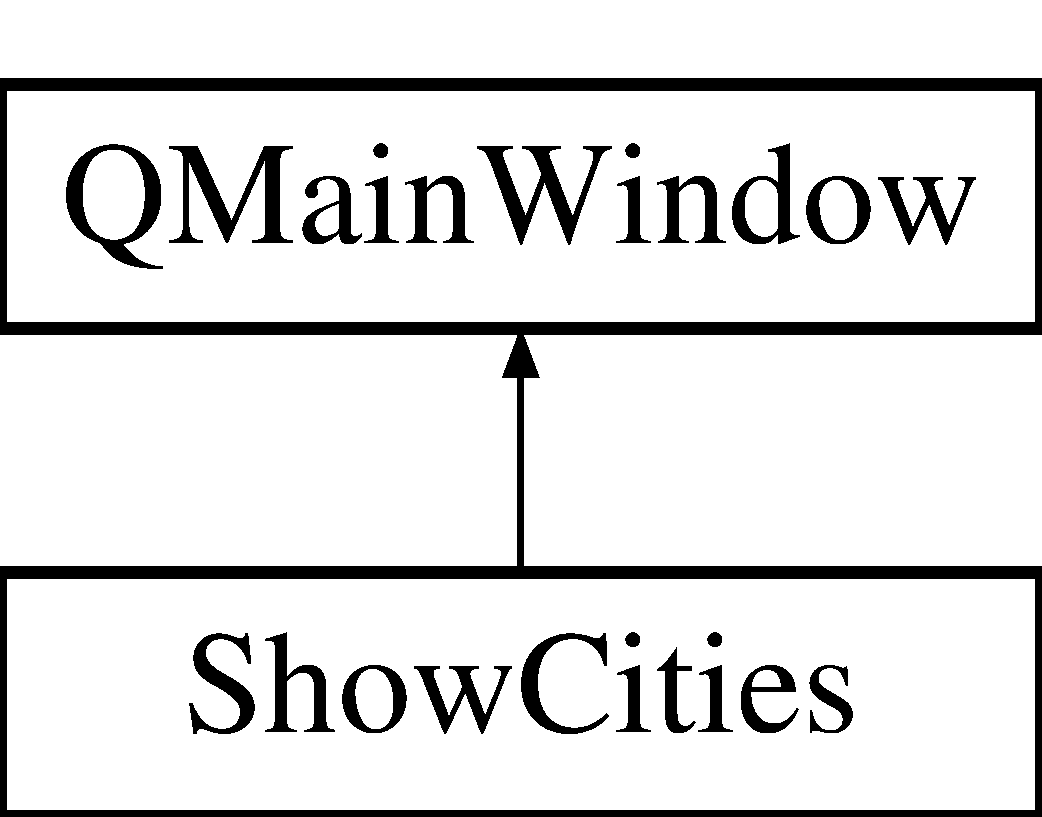
\includegraphics[height=2.000000cm]{class_show_cities}
\end{center}
\end{figure}
\subsection*{Public Member Functions}
\begin{DoxyCompactItemize}
\item 
\hyperlink{class_show_cities_a71a514390bebd22b5e6ecbb6b731979a}{Show\+Cities} (Q\+String title, \hyperlink{classpsql}{psql} $\ast$pg, Q\+Widget $\ast$parent=0)
\begin{DoxyCompactList}\small\item\em \hyperlink{class_show_cities}{Show\+Cities} The Show\+Citis class constructor. \end{DoxyCompactList}\item 
\mbox{\Hypertarget{class_show_cities_a8026675035c0bce6dab846262e1da0c5}\label{class_show_cities_a8026675035c0bce6dab846262e1da0c5}} 
void \hyperlink{class_show_cities_a8026675035c0bce6dab846262e1da0c5}{get\+Cities} ()
\begin{DoxyCompactList}\small\item\em \hyperlink{class_show_cities_a8026675035c0bce6dab846262e1da0c5}{Show\+Cities\+::get\+Cities} Builds a list to be used in the combobox of city I\+Ds based on registered cities in the database. \end{DoxyCompactList}\item 
void \hyperlink{class_show_cities_af191eeab72b3bdd74f0e710face98292}{get\+City} (int city\+Name)
\begin{DoxyCompactList}\small\item\em \hyperlink{class_show_cities_af191eeab72b3bdd74f0e710face98292}{Show\+Cities\+::get\+City} Shows data about the current city based on the ID. \end{DoxyCompactList}\item 
void \hyperlink{class_show_cities_acd17480ad6a64e989e9aa0b07d30141b}{set\+City\+ID} (int new\+ID)
\begin{DoxyCompactList}\small\item\em \hyperlink{class_show_cities_acd17480ad6a64e989e9aa0b07d30141b}{Show\+Cities\+::set\+City\+ID} Sets a new city ID. \end{DoxyCompactList}\item 
void \hyperlink{class_show_cities_acadd6c1bdb26d30e796bab4b5b2acfd9}{set\+City\+Name} (Q\+String new\+Name)
\begin{DoxyCompactList}\small\item\em \hyperlink{class_show_cities_acadd6c1bdb26d30e796bab4b5b2acfd9}{Show\+Cities\+::set\+City\+Name} Sets the name of the city. \end{DoxyCompactList}\item 
void \hyperlink{class_show_cities_a853a958ebc2c0d42d872c237d431fe25}{set\+Country\+ID} (int new\+ID)
\begin{DoxyCompactList}\small\item\em \hyperlink{class_show_cities_a853a958ebc2c0d42d872c237d431fe25}{Show\+Cities\+::set\+Country\+ID} Sets the ID of the country in which the city exists. \end{DoxyCompactList}\item 
void \hyperlink{class_show_cities_a6974ab22950cede9fb290490bcc8f3a5}{set\+Country\+Name} (Q\+String new\+Name)
\begin{DoxyCompactList}\small\item\em \hyperlink{class_show_cities_a6974ab22950cede9fb290490bcc8f3a5}{Show\+Cities\+::set\+Country\+Name} Sets the name of the country where the current city is located. \end{DoxyCompactList}\item 
int \hyperlink{class_show_cities_ac81b38d6862643619d07f82fe12b5c02}{get\+City\+ID} ()
\begin{DoxyCompactList}\small\item\em \hyperlink{class_show_cities_ac81b38d6862643619d07f82fe12b5c02}{Show\+Cities\+::get\+City\+ID} Gets the current city ID. \end{DoxyCompactList}\item 
\mbox{\Hypertarget{class_show_cities_a8fa42e8a5b12579cd04ae2a8ee4a9370}\label{class_show_cities_a8fa42e8a5b12579cd04ae2a8ee4a9370}} 
void \hyperlink{class_show_cities_a8fa42e8a5b12579cd04ae2a8ee4a9370}{get\+Country\+I\+Ds} ()
\begin{DoxyCompactList}\small\item\em \hyperlink{class_show_cities_a8fa42e8a5b12579cd04ae2a8ee4a9370}{Show\+Cities\+::get\+Country\+I\+Ds} Builds a list of countries based on existing data in the database. That data will be used to fill the combo\+Box\+Country\+ID. \end{DoxyCompactList}\item 
int \hyperlink{class_show_cities_a8f66380734928e926a732a0088c1d998}{get\+Country\+ID} ()
\begin{DoxyCompactList}\small\item\em \hyperlink{class_show_cities_a8f66380734928e926a732a0088c1d998}{Show\+Cities\+::get\+Country\+ID} Gets the ID of the country where the current city is located. \end{DoxyCompactList}\item 
Q\+String \hyperlink{class_show_cities_a3640b91c66939d0070c3dd6f5b9eb93c}{get\+City\+Name} ()
\begin{DoxyCompactList}\small\item\em \hyperlink{class_show_cities_a3640b91c66939d0070c3dd6f5b9eb93c}{Show\+Cities\+::get\+City\+Name} Gets the name of the current city. \end{DoxyCompactList}\item 
Q\+String \hyperlink{class_show_cities_a93cf32e7ef19a182d0022c9c888392aa}{get\+Country\+Name} ()
\begin{DoxyCompactList}\small\item\em \hyperlink{class_show_cities_a93cf32e7ef19a182d0022c9c888392aa}{Show\+Cities\+::get\+Country\+Name} Gets the name of the country where the current city is located. \end{DoxyCompactList}\end{DoxyCompactItemize}


\subsection{Detailed Description}
The \hyperlink{class_show_cities}{Show\+Cities} class. 

\subsection{Constructor \& Destructor Documentation}
\mbox{\Hypertarget{class_show_cities_a71a514390bebd22b5e6ecbb6b731979a}\label{class_show_cities_a71a514390bebd22b5e6ecbb6b731979a}} 
\index{Show\+Cities@{Show\+Cities}!Show\+Cities@{Show\+Cities}}
\index{Show\+Cities@{Show\+Cities}!Show\+Cities@{Show\+Cities}}
\subsubsection{\texorpdfstring{Show\+Cities()}{ShowCities()}}
{\footnotesize\ttfamily Show\+Cities\+::\+Show\+Cities (\begin{DoxyParamCaption}\item[{Q\+String}]{window\+Title,  }\item[{\hyperlink{classpsql}{psql} $\ast$}]{pg,  }\item[{Q\+Widget $\ast$}]{parent = {\ttfamily 0} }\end{DoxyParamCaption})\hspace{0.3cm}{\ttfamily [explicit]}}



\hyperlink{class_show_cities}{Show\+Cities} The Show\+Citis class constructor. 


\begin{DoxyParams}{Parameters}
{\em window\+Title} & The title to be used in windows, message boxes and other things. \\
\hline
{\em pg} & A pointer to the Postgre\+S\+QL database \\
\hline
{\em parent} & \\
\hline
\end{DoxyParams}


\subsection{Member Function Documentation}
\mbox{\Hypertarget{class_show_cities_af191eeab72b3bdd74f0e710face98292}\label{class_show_cities_af191eeab72b3bdd74f0e710face98292}} 
\index{Show\+Cities@{Show\+Cities}!get\+City@{get\+City}}
\index{get\+City@{get\+City}!Show\+Cities@{Show\+Cities}}
\subsubsection{\texorpdfstring{get\+City()}{getCity()}}
{\footnotesize\ttfamily void Show\+Cities\+::get\+City (\begin{DoxyParamCaption}\item[{int}]{city\+ID }\end{DoxyParamCaption})}



\hyperlink{class_show_cities_af191eeab72b3bdd74f0e710face98292}{Show\+Cities\+::get\+City} Shows data about the current city based on the ID. 


\begin{DoxyParams}{Parameters}
{\em city\+ID} & The ID of the city in question. \\
\hline
\end{DoxyParams}
\mbox{\Hypertarget{class_show_cities_ac81b38d6862643619d07f82fe12b5c02}\label{class_show_cities_ac81b38d6862643619d07f82fe12b5c02}} 
\index{Show\+Cities@{Show\+Cities}!get\+City\+ID@{get\+City\+ID}}
\index{get\+City\+ID@{get\+City\+ID}!Show\+Cities@{Show\+Cities}}
\subsubsection{\texorpdfstring{get\+City\+I\+D()}{getCityID()}}
{\footnotesize\ttfamily int Show\+Cities\+::get\+City\+ID (\begin{DoxyParamCaption}{ }\end{DoxyParamCaption})}



\hyperlink{class_show_cities_ac81b38d6862643619d07f82fe12b5c02}{Show\+Cities\+::get\+City\+ID} Gets the current city ID. 

\begin{DoxyReturn}{Returns}
The city ID. 
\end{DoxyReturn}
\mbox{\Hypertarget{class_show_cities_a3640b91c66939d0070c3dd6f5b9eb93c}\label{class_show_cities_a3640b91c66939d0070c3dd6f5b9eb93c}} 
\index{Show\+Cities@{Show\+Cities}!get\+City\+Name@{get\+City\+Name}}
\index{get\+City\+Name@{get\+City\+Name}!Show\+Cities@{Show\+Cities}}
\subsubsection{\texorpdfstring{get\+City\+Name()}{getCityName()}}
{\footnotesize\ttfamily Q\+String Show\+Cities\+::get\+City\+Name (\begin{DoxyParamCaption}{ }\end{DoxyParamCaption})}



\hyperlink{class_show_cities_a3640b91c66939d0070c3dd6f5b9eb93c}{Show\+Cities\+::get\+City\+Name} Gets the name of the current city. 

\begin{DoxyReturn}{Returns}
The name of the city 
\end{DoxyReturn}
\mbox{\Hypertarget{class_show_cities_a8f66380734928e926a732a0088c1d998}\label{class_show_cities_a8f66380734928e926a732a0088c1d998}} 
\index{Show\+Cities@{Show\+Cities}!get\+Country\+ID@{get\+Country\+ID}}
\index{get\+Country\+ID@{get\+Country\+ID}!Show\+Cities@{Show\+Cities}}
\subsubsection{\texorpdfstring{get\+Country\+I\+D()}{getCountryID()}}
{\footnotesize\ttfamily int Show\+Cities\+::get\+Country\+ID (\begin{DoxyParamCaption}{ }\end{DoxyParamCaption})}



\hyperlink{class_show_cities_a8f66380734928e926a732a0088c1d998}{Show\+Cities\+::get\+Country\+ID} Gets the ID of the country where the current city is located. 

\begin{DoxyReturn}{Returns}
The country ID. 
\end{DoxyReturn}
\mbox{\Hypertarget{class_show_cities_a93cf32e7ef19a182d0022c9c888392aa}\label{class_show_cities_a93cf32e7ef19a182d0022c9c888392aa}} 
\index{Show\+Cities@{Show\+Cities}!get\+Country\+Name@{get\+Country\+Name}}
\index{get\+Country\+Name@{get\+Country\+Name}!Show\+Cities@{Show\+Cities}}
\subsubsection{\texorpdfstring{get\+Country\+Name()}{getCountryName()}}
{\footnotesize\ttfamily Q\+String Show\+Cities\+::get\+Country\+Name (\begin{DoxyParamCaption}{ }\end{DoxyParamCaption})}



\hyperlink{class_show_cities_a93cf32e7ef19a182d0022c9c888392aa}{Show\+Cities\+::get\+Country\+Name} Gets the name of the country where the current city is located. 

\begin{DoxyReturn}{Returns}
The country name 
\end{DoxyReturn}
\mbox{\Hypertarget{class_show_cities_acd17480ad6a64e989e9aa0b07d30141b}\label{class_show_cities_acd17480ad6a64e989e9aa0b07d30141b}} 
\index{Show\+Cities@{Show\+Cities}!set\+City\+ID@{set\+City\+ID}}
\index{set\+City\+ID@{set\+City\+ID}!Show\+Cities@{Show\+Cities}}
\subsubsection{\texorpdfstring{set\+City\+I\+D()}{setCityID()}}
{\footnotesize\ttfamily void Show\+Cities\+::set\+City\+ID (\begin{DoxyParamCaption}\item[{int}]{new\+ID }\end{DoxyParamCaption})}



\hyperlink{class_show_cities_acd17480ad6a64e989e9aa0b07d30141b}{Show\+Cities\+::set\+City\+ID} Sets a new city ID. 


\begin{DoxyParams}{Parameters}
{\em new\+ID} & The ID of the new city in question. \\
\hline
\end{DoxyParams}
\mbox{\Hypertarget{class_show_cities_acadd6c1bdb26d30e796bab4b5b2acfd9}\label{class_show_cities_acadd6c1bdb26d30e796bab4b5b2acfd9}} 
\index{Show\+Cities@{Show\+Cities}!set\+City\+Name@{set\+City\+Name}}
\index{set\+City\+Name@{set\+City\+Name}!Show\+Cities@{Show\+Cities}}
\subsubsection{\texorpdfstring{set\+City\+Name()}{setCityName()}}
{\footnotesize\ttfamily void Show\+Cities\+::set\+City\+Name (\begin{DoxyParamCaption}\item[{Q\+String}]{new\+Name }\end{DoxyParamCaption})}



\hyperlink{class_show_cities_acadd6c1bdb26d30e796bab4b5b2acfd9}{Show\+Cities\+::set\+City\+Name} Sets the name of the city. 


\begin{DoxyParams}{Parameters}
{\em new\+Name} & The new city name to be used. \\
\hline
\end{DoxyParams}
\mbox{\Hypertarget{class_show_cities_a853a958ebc2c0d42d872c237d431fe25}\label{class_show_cities_a853a958ebc2c0d42d872c237d431fe25}} 
\index{Show\+Cities@{Show\+Cities}!set\+Country\+ID@{set\+Country\+ID}}
\index{set\+Country\+ID@{set\+Country\+ID}!Show\+Cities@{Show\+Cities}}
\subsubsection{\texorpdfstring{set\+Country\+I\+D()}{setCountryID()}}
{\footnotesize\ttfamily void Show\+Cities\+::set\+Country\+ID (\begin{DoxyParamCaption}\item[{int}]{new\+ID }\end{DoxyParamCaption})}



\hyperlink{class_show_cities_a853a958ebc2c0d42d872c237d431fe25}{Show\+Cities\+::set\+Country\+ID} Sets the ID of the country in which the city exists. 


\begin{DoxyParams}{Parameters}
{\em new\+ID} & The new country ID \\
\hline
\end{DoxyParams}
\mbox{\Hypertarget{class_show_cities_a6974ab22950cede9fb290490bcc8f3a5}\label{class_show_cities_a6974ab22950cede9fb290490bcc8f3a5}} 
\index{Show\+Cities@{Show\+Cities}!set\+Country\+Name@{set\+Country\+Name}}
\index{set\+Country\+Name@{set\+Country\+Name}!Show\+Cities@{Show\+Cities}}
\subsubsection{\texorpdfstring{set\+Country\+Name()}{setCountryName()}}
{\footnotesize\ttfamily void Show\+Cities\+::set\+Country\+Name (\begin{DoxyParamCaption}\item[{Q\+String}]{new\+Name }\end{DoxyParamCaption})}



\hyperlink{class_show_cities_a6974ab22950cede9fb290490bcc8f3a5}{Show\+Cities\+::set\+Country\+Name} Sets the name of the country where the current city is located. 


\begin{DoxyParams}{Parameters}
{\em new\+Name} & The name of the country. \\
\hline
\end{DoxyParams}


The documentation for this class was generated from the following files\+:\begin{DoxyCompactItemize}
\item 
showcities.\+h\item 
showcities.\+cpp\end{DoxyCompactItemize}

\hypertarget{class_show_countries}{}\section{Show\+Countries Class Reference}
\label{class_show_countries}\index{ShowCountries@{ShowCountries}}
Inheritance diagram for Show\+Countries\+:\begin{figure}[H]
\begin{center}
\leavevmode
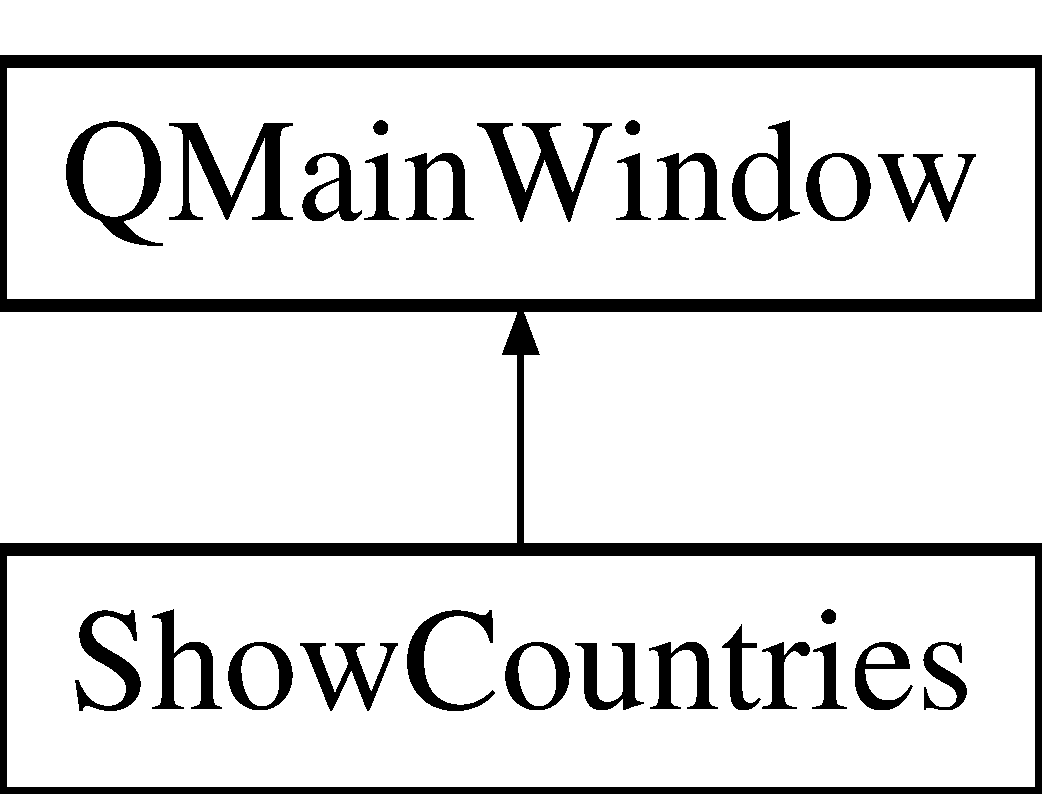
\includegraphics[height=2.000000cm]{class_show_countries}
\end{center}
\end{figure}
\subsection*{Public Member Functions}
\begin{DoxyCompactItemize}
\item 
\mbox{\hyperlink{class_show_countries_a509e0b6ebeb2fb580e7985b81b3f77e6}{Show\+Countries}} (Q\+String window\+Title, \mbox{\hyperlink{classpsql}{psql}} $\ast$pg, Q\+Widget $\ast$parent=0)
\begin{DoxyCompactList}\small\item\em \mbox{\hyperlink{class_show_countries}{Show\+Countries}} The \mbox{\hyperlink{class_show_countries}{Show\+Countries}} class constructor. \end{DoxyCompactList}\item 
\mbox{\Hypertarget{class_show_countries_a93e4a320155473e2af80476f5a4648a3}\label{class_show_countries_a93e4a320155473e2af80476f5a4648a3}} 
void \mbox{\hyperlink{class_show_countries_a93e4a320155473e2af80476f5a4648a3}{get\+Countries}} ()
\begin{DoxyCompactList}\small\item\em \mbox{\hyperlink{class_show_countries_a93e4a320155473e2af80476f5a4648a3}{Show\+Countries\+::get\+Countries}} Builds a Q\+Linked\+List of integers. This list is then added to the combobox. \end{DoxyCompactList}\item 
void \mbox{\hyperlink{class_show_countries_a5f39325688b0e71fa613d5b33810ce02}{get\+Country}} (int country\+ID)
\begin{DoxyCompactList}\small\item\em \mbox{\hyperlink{class_show_countries_a5f39325688b0e71fa613d5b33810ce02}{Show\+Countries\+::get\+Country}} Fetches information about the current country and fills the combobox and textbox with the new information. \end{DoxyCompactList}\item 
int \mbox{\hyperlink{class_show_countries_a02956713871e89645487500f3c9b77b8}{get\+Country\+ID}} ()
\begin{DoxyCompactList}\small\item\em \mbox{\hyperlink{class_show_countries_a02956713871e89645487500f3c9b77b8}{Show\+Countries\+::get\+Country\+ID}} Gets the ID of the current country. \end{DoxyCompactList}\item 
Q\+String \mbox{\hyperlink{class_show_countries_afc6d5f6817bd4c9388aef3d52d09d768}{get\+Country\+Name}} ()
\begin{DoxyCompactList}\small\item\em \mbox{\hyperlink{class_show_countries_afc6d5f6817bd4c9388aef3d52d09d768}{Show\+Countries\+::get\+Country\+Name}} Gets the name of the current country. \end{DoxyCompactList}\item 
void \mbox{\hyperlink{class_show_countries_a751b9d3c6859102f48d3ecc254135906}{set\+Country\+ID}} (int new\+ID)
\begin{DoxyCompactList}\small\item\em \mbox{\hyperlink{class_show_countries_a751b9d3c6859102f48d3ecc254135906}{Show\+Countries\+::set\+Country\+ID}} Sets the current identification number of a country. \end{DoxyCompactList}\item 
void \mbox{\hyperlink{class_show_countries_aefa9daeff484f4028ea5a280b280dd36}{set\+Country\+Name}} (Q\+String new\+Name)
\begin{DoxyCompactList}\small\item\em \mbox{\hyperlink{class_show_countries_aefa9daeff484f4028ea5a280b280dd36}{Show\+Countries\+::set\+Country\+Name}} Sets a new name of the current country. \end{DoxyCompactList}\end{DoxyCompactItemize}


\subsection{Constructor \& Destructor Documentation}
\mbox{\Hypertarget{class_show_countries_a509e0b6ebeb2fb580e7985b81b3f77e6}\label{class_show_countries_a509e0b6ebeb2fb580e7985b81b3f77e6}} 
\index{ShowCountries@{ShowCountries}!ShowCountries@{ShowCountries}}
\index{ShowCountries@{ShowCountries}!ShowCountries@{ShowCountries}}
\subsubsection{\texorpdfstring{ShowCountries()}{ShowCountries()}}
{\footnotesize\ttfamily Show\+Countries\+::\+Show\+Countries (\begin{DoxyParamCaption}\item[{Q\+String}]{window\+Title,  }\item[{\mbox{\hyperlink{classpsql}{psql}} $\ast$}]{pg,  }\item[{Q\+Widget $\ast$}]{parent = {\ttfamily 0} }\end{DoxyParamCaption})\hspace{0.3cm}{\ttfamily [explicit]}}



\mbox{\hyperlink{class_show_countries}{Show\+Countries}} The \mbox{\hyperlink{class_show_countries}{Show\+Countries}} class constructor. 


\begin{DoxyParams}{Parameters}
{\em window\+Title} & The title to be used with message boxes (Q\+Message\+Box) \\
\hline
{\em pg} & A pointer to the Postgre\+S\+QL database class. \\
\hline
{\em parent} & \\
\hline
\end{DoxyParams}


\subsection{Member Function Documentation}
\mbox{\Hypertarget{class_show_countries_a5f39325688b0e71fa613d5b33810ce02}\label{class_show_countries_a5f39325688b0e71fa613d5b33810ce02}} 
\index{ShowCountries@{ShowCountries}!getCountry@{getCountry}}
\index{getCountry@{getCountry}!ShowCountries@{ShowCountries}}
\subsubsection{\texorpdfstring{getCountry()}{getCountry()}}
{\footnotesize\ttfamily void Show\+Countries\+::get\+Country (\begin{DoxyParamCaption}\item[{int}]{country\+ID }\end{DoxyParamCaption})}



\mbox{\hyperlink{class_show_countries_a5f39325688b0e71fa613d5b33810ce02}{Show\+Countries\+::get\+Country}} Fetches information about the current country and fills the combobox and textbox with the new information. 


\begin{DoxyParams}{Parameters}
{\em country\+ID} & The ID of the country in question. \\
\hline
\end{DoxyParams}
\mbox{\Hypertarget{class_show_countries_a02956713871e89645487500f3c9b77b8}\label{class_show_countries_a02956713871e89645487500f3c9b77b8}} 
\index{ShowCountries@{ShowCountries}!getCountryID@{getCountryID}}
\index{getCountryID@{getCountryID}!ShowCountries@{ShowCountries}}
\subsubsection{\texorpdfstring{getCountryID()}{getCountryID()}}
{\footnotesize\ttfamily int Show\+Countries\+::get\+Country\+ID (\begin{DoxyParamCaption}{ }\end{DoxyParamCaption})}



\mbox{\hyperlink{class_show_countries_a02956713871e89645487500f3c9b77b8}{Show\+Countries\+::get\+Country\+ID}} Gets the ID of the current country. 

\begin{DoxyReturn}{Returns}
The identification number to be returned 
\end{DoxyReturn}
\mbox{\Hypertarget{class_show_countries_afc6d5f6817bd4c9388aef3d52d09d768}\label{class_show_countries_afc6d5f6817bd4c9388aef3d52d09d768}} 
\index{ShowCountries@{ShowCountries}!getCountryName@{getCountryName}}
\index{getCountryName@{getCountryName}!ShowCountries@{ShowCountries}}
\subsubsection{\texorpdfstring{getCountryName()}{getCountryName()}}
{\footnotesize\ttfamily Q\+String Show\+Countries\+::get\+Country\+Name (\begin{DoxyParamCaption}{ }\end{DoxyParamCaption})}



\mbox{\hyperlink{class_show_countries_afc6d5f6817bd4c9388aef3d52d09d768}{Show\+Countries\+::get\+Country\+Name}} Gets the name of the current country. 

\begin{DoxyReturn}{Returns}
The name of the country 
\end{DoxyReturn}
\mbox{\Hypertarget{class_show_countries_a751b9d3c6859102f48d3ecc254135906}\label{class_show_countries_a751b9d3c6859102f48d3ecc254135906}} 
\index{ShowCountries@{ShowCountries}!setCountryID@{setCountryID}}
\index{setCountryID@{setCountryID}!ShowCountries@{ShowCountries}}
\subsubsection{\texorpdfstring{setCountryID()}{setCountryID()}}
{\footnotesize\ttfamily void Show\+Countries\+::set\+Country\+ID (\begin{DoxyParamCaption}\item[{int}]{new\+ID }\end{DoxyParamCaption})}



\mbox{\hyperlink{class_show_countries_a751b9d3c6859102f48d3ecc254135906}{Show\+Countries\+::set\+Country\+ID}} Sets the current identification number of a country. 


\begin{DoxyParams}{Parameters}
{\em new\+ID} & The new country ID \\
\hline
\end{DoxyParams}
\mbox{\Hypertarget{class_show_countries_aefa9daeff484f4028ea5a280b280dd36}\label{class_show_countries_aefa9daeff484f4028ea5a280b280dd36}} 
\index{ShowCountries@{ShowCountries}!setCountryName@{setCountryName}}
\index{setCountryName@{setCountryName}!ShowCountries@{ShowCountries}}
\subsubsection{\texorpdfstring{setCountryName()}{setCountryName()}}
{\footnotesize\ttfamily void Show\+Countries\+::set\+Country\+Name (\begin{DoxyParamCaption}\item[{Q\+String}]{new\+Name }\end{DoxyParamCaption})}



\mbox{\hyperlink{class_show_countries_aefa9daeff484f4028ea5a280b280dd36}{Show\+Countries\+::set\+Country\+Name}} Sets a new name of the current country. 


\begin{DoxyParams}{Parameters}
{\em new\+Name} & The new name of the country \\
\hline
\end{DoxyParams}


The documentation for this class was generated from the following files\+:\begin{DoxyCompactItemize}
\item 
showcountries.\+h\item 
showcountries.\+cpp\end{DoxyCompactItemize}

\hypertarget{class_show_statuses}{}\section{Show\+Statuses Class Reference}
\label{class_show_statuses}\index{Show\+Statuses@{Show\+Statuses}}


The \hyperlink{class_show_statuses}{Show\+Statuses} class.  




{\ttfamily \#include $<$showstatuses.\+h$>$}

Inheritance diagram for Show\+Statuses\+:\begin{figure}[H]
\begin{center}
\leavevmode
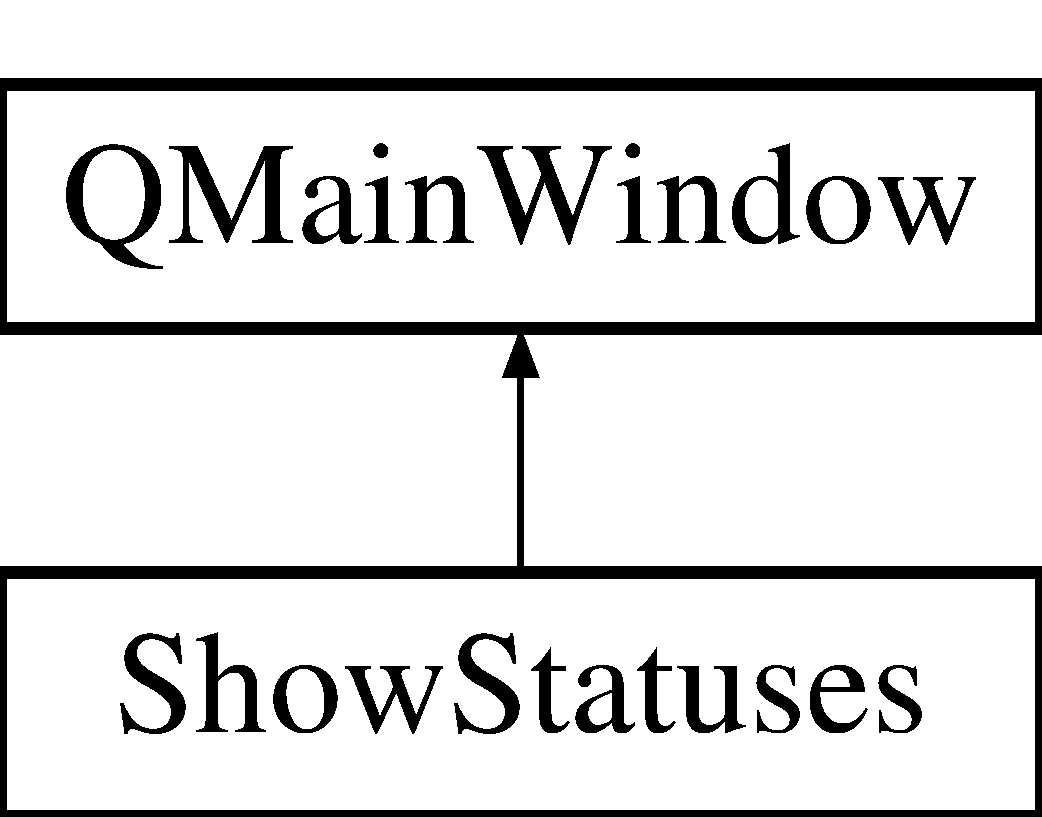
\includegraphics[height=2.000000cm]{class_show_statuses}
\end{center}
\end{figure}
\subsection*{Public Member Functions}
\begin{DoxyCompactItemize}
\item 
\hyperlink{class_show_statuses_a5f33b2e8d68add734ceb466de0fc80ae}{Show\+Statuses} (Q\+String window\+Title, \hyperlink{classpsql}{psql} $\ast$pg, Q\+Widget $\ast$parent=0)
\begin{DoxyCompactList}\small\item\em \hyperlink{class_show_statuses}{Show\+Statuses} The \hyperlink{class_show_statuses}{Show\+Statuses} class constructor. \end{DoxyCompactList}\item 
void \hyperlink{class_show_statuses_a688fb68ab4f0e65666b61137aa70aed9}{get\+Status} (int status\+ID)
\begin{DoxyCompactList}\small\item\em \hyperlink{class_show_statuses_a688fb68ab4f0e65666b61137aa70aed9}{Show\+Statuses\+::get\+Status} Fetches information from the database about the current status and fills the combobox and textbox with appropriate data. \end{DoxyCompactList}\item 
\mbox{\Hypertarget{class_show_statuses_a78ceb898d01bd2892e1ef942672666ec}\label{class_show_statuses_a78ceb898d01bd2892e1ef942672666ec}} 
void \hyperlink{class_show_statuses_a78ceb898d01bd2892e1ef942672666ec}{get\+Statuses} ()
\begin{DoxyCompactList}\small\item\em \hyperlink{class_show_statuses_a78ceb898d01bd2892e1ef942672666ec}{Show\+Statuses\+::get\+Statuses} Builds a list of all status I\+Ds in the database. This list is then added to the combo\+Box\+Status\+ID. \end{DoxyCompactList}\item 
int \hyperlink{class_show_statuses_accb269831b12a839751cb7ae2822dfe1}{get\+Status\+ID} ()
\begin{DoxyCompactList}\small\item\em get\+Status\+ID Gets the ID of the current status \end{DoxyCompactList}\item 
Q\+String \hyperlink{class_show_statuses_a311ebb73bbc52089506fb31d7936bcb3}{get\+Status\+Name} ()
\begin{DoxyCompactList}\small\item\em \hyperlink{class_show_statuses_a311ebb73bbc52089506fb31d7936bcb3}{Show\+Statuses\+::get\+Status\+Name} Gets the name of the current status. \end{DoxyCompactList}\item 
void \hyperlink{class_show_statuses_a03eb52c13df7220ced551be7be69f822}{set\+Status\+ID} (int new\+ID)
\begin{DoxyCompactList}\small\item\em \hyperlink{class_show_statuses_a03eb52c13df7220ced551be7be69f822}{Show\+Statuses\+::set\+Status\+ID} Changes the current status ID. \end{DoxyCompactList}\item 
void \hyperlink{class_show_statuses_ac4a3c02814d6a326a0d0a6bfc8239483}{set\+Status\+Name} (Q\+String new\+Name)
\begin{DoxyCompactList}\small\item\em \hyperlink{class_show_statuses_ac4a3c02814d6a326a0d0a6bfc8239483}{Show\+Statuses\+::set\+Status\+Name} Changes the name of the current status. \end{DoxyCompactList}\end{DoxyCompactItemize}


\subsection{Detailed Description}
The \hyperlink{class_show_statuses}{Show\+Statuses} class. 

\subsection{Constructor \& Destructor Documentation}
\mbox{\Hypertarget{class_show_statuses_a5f33b2e8d68add734ceb466de0fc80ae}\label{class_show_statuses_a5f33b2e8d68add734ceb466de0fc80ae}} 
\index{Show\+Statuses@{Show\+Statuses}!Show\+Statuses@{Show\+Statuses}}
\index{Show\+Statuses@{Show\+Statuses}!Show\+Statuses@{Show\+Statuses}}
\subsubsection{\texorpdfstring{Show\+Statuses()}{ShowStatuses()}}
{\footnotesize\ttfamily Show\+Statuses\+::\+Show\+Statuses (\begin{DoxyParamCaption}\item[{Q\+String}]{window\+Title,  }\item[{\hyperlink{classpsql}{psql} $\ast$}]{pg,  }\item[{Q\+Widget $\ast$}]{parent = {\ttfamily 0} }\end{DoxyParamCaption})\hspace{0.3cm}{\ttfamily [explicit]}}



\hyperlink{class_show_statuses}{Show\+Statuses} The \hyperlink{class_show_statuses}{Show\+Statuses} class constructor. 

\hyperlink{class_show_statuses_a5f33b2e8d68add734ceb466de0fc80ae}{Show\+Statuses\+::\+Show\+Statuses} The \hyperlink{class_show_statuses}{Show\+Statuses} class constructor.


\begin{DoxyParams}{Parameters}
{\em window\+Title} & The title to be used with message boxes (Q\+Message\+Box) \\
\hline
{\em pg} & A pointer to the Postgre\+S\+QL database. \\
\hline
{\em parent} & \\
\hline
{\em window\+Title} & The title to be used with message boxes (Q\+Message\+Box) \\
\hline
{\em pg} & A pointer to the Postgre\+S\+QL database class. \\
\hline
{\em parent} & \\
\hline
\end{DoxyParams}


\subsection{Member Function Documentation}
\mbox{\Hypertarget{class_show_statuses_a688fb68ab4f0e65666b61137aa70aed9}\label{class_show_statuses_a688fb68ab4f0e65666b61137aa70aed9}} 
\index{Show\+Statuses@{Show\+Statuses}!get\+Status@{get\+Status}}
\index{get\+Status@{get\+Status}!Show\+Statuses@{Show\+Statuses}}
\subsubsection{\texorpdfstring{get\+Status()}{getStatus()}}
{\footnotesize\ttfamily void Show\+Statuses\+::get\+Status (\begin{DoxyParamCaption}\item[{int}]{status\+ID }\end{DoxyParamCaption})}



\hyperlink{class_show_statuses_a688fb68ab4f0e65666b61137aa70aed9}{Show\+Statuses\+::get\+Status} Fetches information from the database about the current status and fills the combobox and textbox with appropriate data. 


\begin{DoxyParams}{Parameters}
{\em status\+ID} & The identification number of the status in question. \\
\hline
\end{DoxyParams}
\mbox{\Hypertarget{class_show_statuses_accb269831b12a839751cb7ae2822dfe1}\label{class_show_statuses_accb269831b12a839751cb7ae2822dfe1}} 
\index{Show\+Statuses@{Show\+Statuses}!get\+Status\+ID@{get\+Status\+ID}}
\index{get\+Status\+ID@{get\+Status\+ID}!Show\+Statuses@{Show\+Statuses}}
\subsubsection{\texorpdfstring{get\+Status\+I\+D()}{getStatusID()}}
{\footnotesize\ttfamily int Show\+Statuses\+::get\+Status\+ID (\begin{DoxyParamCaption}{ }\end{DoxyParamCaption})}



get\+Status\+ID Gets the ID of the current status 

\hyperlink{class_show_statuses_accb269831b12a839751cb7ae2822dfe1}{Show\+Statuses\+::get\+Status\+ID} Gets the identification number of the current status.

\begin{DoxyReturn}{Returns}
The status identification number

The ID of the current status. 
\end{DoxyReturn}
\mbox{\Hypertarget{class_show_statuses_a311ebb73bbc52089506fb31d7936bcb3}\label{class_show_statuses_a311ebb73bbc52089506fb31d7936bcb3}} 
\index{Show\+Statuses@{Show\+Statuses}!get\+Status\+Name@{get\+Status\+Name}}
\index{get\+Status\+Name@{get\+Status\+Name}!Show\+Statuses@{Show\+Statuses}}
\subsubsection{\texorpdfstring{get\+Status\+Name()}{getStatusName()}}
{\footnotesize\ttfamily Q\+String Show\+Statuses\+::get\+Status\+Name (\begin{DoxyParamCaption}{ }\end{DoxyParamCaption})}



\hyperlink{class_show_statuses_a311ebb73bbc52089506fb31d7936bcb3}{Show\+Statuses\+::get\+Status\+Name} Gets the name of the current status. 

\begin{DoxyReturn}{Returns}
The current status name 
\end{DoxyReturn}
\mbox{\Hypertarget{class_show_statuses_a03eb52c13df7220ced551be7be69f822}\label{class_show_statuses_a03eb52c13df7220ced551be7be69f822}} 
\index{Show\+Statuses@{Show\+Statuses}!set\+Status\+ID@{set\+Status\+ID}}
\index{set\+Status\+ID@{set\+Status\+ID}!Show\+Statuses@{Show\+Statuses}}
\subsubsection{\texorpdfstring{set\+Status\+I\+D()}{setStatusID()}}
{\footnotesize\ttfamily void Show\+Statuses\+::set\+Status\+ID (\begin{DoxyParamCaption}\item[{int}]{new\+ID }\end{DoxyParamCaption})}



\hyperlink{class_show_statuses_a03eb52c13df7220ced551be7be69f822}{Show\+Statuses\+::set\+Status\+ID} Changes the current status ID. 


\begin{DoxyParams}{Parameters}
{\em new\+ID} & The new status ID \\
\hline
\end{DoxyParams}
\mbox{\Hypertarget{class_show_statuses_ac4a3c02814d6a326a0d0a6bfc8239483}\label{class_show_statuses_ac4a3c02814d6a326a0d0a6bfc8239483}} 
\index{Show\+Statuses@{Show\+Statuses}!set\+Status\+Name@{set\+Status\+Name}}
\index{set\+Status\+Name@{set\+Status\+Name}!Show\+Statuses@{Show\+Statuses}}
\subsubsection{\texorpdfstring{set\+Status\+Name()}{setStatusName()}}
{\footnotesize\ttfamily void Show\+Statuses\+::set\+Status\+Name (\begin{DoxyParamCaption}\item[{Q\+String}]{new\+Name }\end{DoxyParamCaption})}



\hyperlink{class_show_statuses_ac4a3c02814d6a326a0d0a6bfc8239483}{Show\+Statuses\+::set\+Status\+Name} Changes the name of the current status. 


\begin{DoxyParams}{Parameters}
{\em new\+Name} & The new status name. \\
\hline
\end{DoxyParams}


The documentation for this class was generated from the following files\+:\begin{DoxyCompactItemize}
\item 
showstatuses.\+h\item 
showstatuses.\+cpp\end{DoxyCompactItemize}

\hypertarget{classstatistics}{}\section{statistics Class Reference}
\label{classstatistics}\index{statistics@{statistics}}
Inheritance diagram for statistics\+:\begin{figure}[H]
\begin{center}
\leavevmode
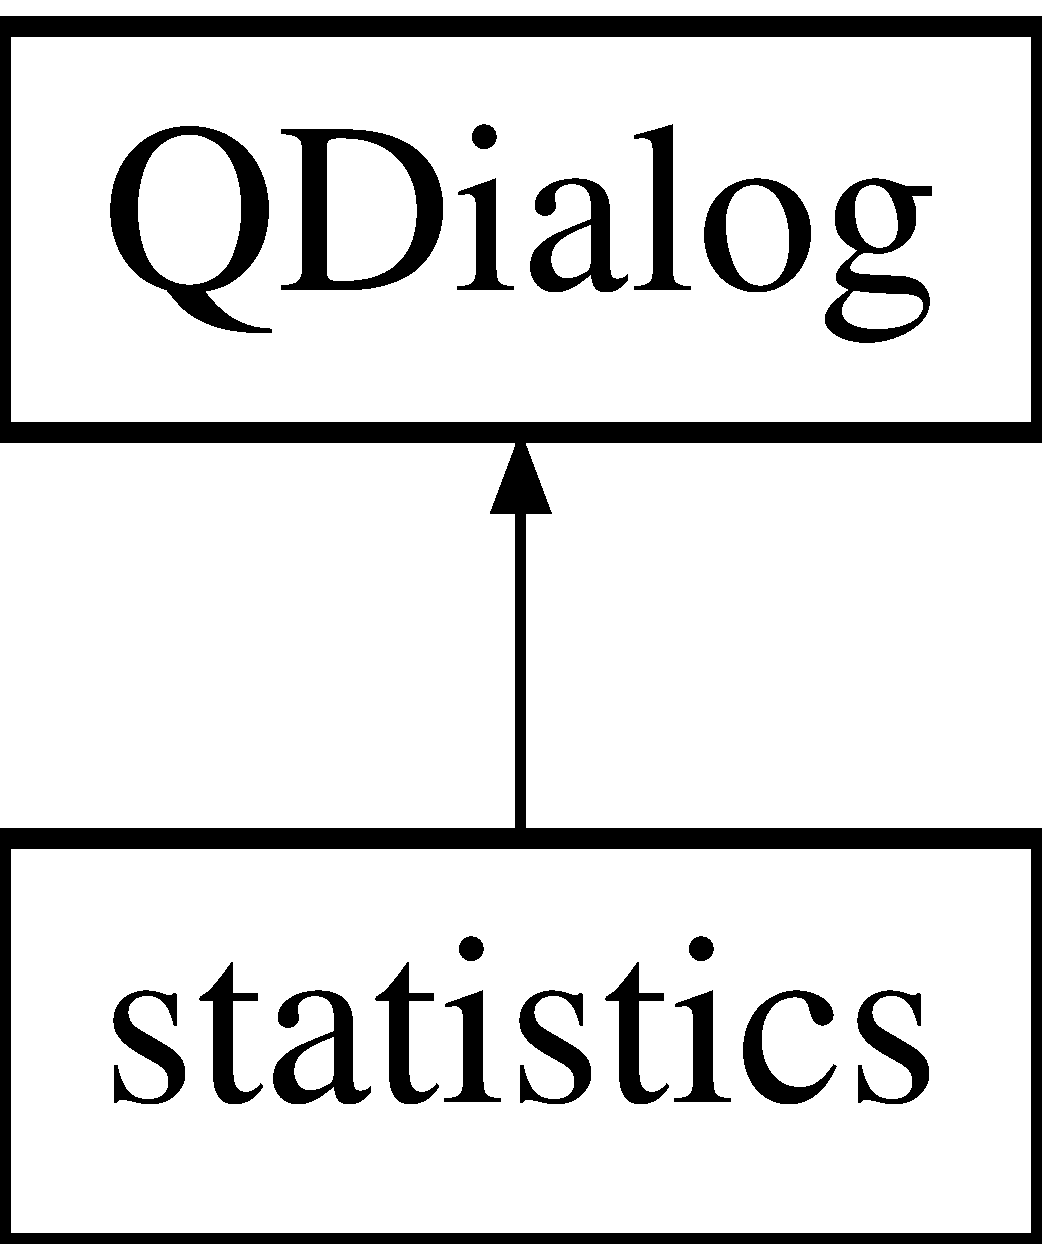
\includegraphics[height=2.000000cm]{classstatistics}
\end{center}
\end{figure}
\subsection*{Public Member Functions}
\begin{DoxyCompactItemize}
\item 
\mbox{\hyperlink{classstatistics_aaa102e49836a3b719df3a82e28735adc}{statistics}} (\mbox{\hyperlink{classpsql}{psql}} $\ast$pg, Q\+Widget $\ast$parent=0)
\begin{DoxyCompactList}\small\item\em \mbox{\hyperlink{classstatistics_aaa102e49836a3b719df3a82e28735adc}{statistics\+::statistics}} statisitcs class constructor. \end{DoxyCompactList}\end{DoxyCompactItemize}


\subsection{Constructor \& Destructor Documentation}
\mbox{\Hypertarget{classstatistics_aaa102e49836a3b719df3a82e28735adc}\label{classstatistics_aaa102e49836a3b719df3a82e28735adc}} 
\index{statistics@{statistics}!statistics@{statistics}}
\index{statistics@{statistics}!statistics@{statistics}}
\subsubsection{\texorpdfstring{statistics()}{statistics()}}
{\footnotesize\ttfamily statistics\+::statistics (\begin{DoxyParamCaption}\item[{\mbox{\hyperlink{classpsql}{psql}} $\ast$}]{pg,  }\item[{Q\+Widget $\ast$}]{parent = {\ttfamily 0} }\end{DoxyParamCaption})\hspace{0.3cm}{\ttfamily [explicit]}}



\mbox{\hyperlink{classstatistics_aaa102e49836a3b719df3a82e28735adc}{statistics\+::statistics}} statisitcs class constructor. 


\begin{DoxyParams}{Parameters}
{\em pg} & The pointer to the psql class \\
\hline
{\em parent} & Pointer the the parent class \\
\hline
\end{DoxyParams}


The documentation for this class was generated from the following files\+:\begin{DoxyCompactItemize}
\item 
statistics.\+h\item 
statistics.\+cpp\end{DoxyCompactItemize}

\hypertarget{classstring_check}{}\section{string\+Check Class Reference}
\label{classstring_check}\index{string\+Check@{string\+Check}}
\subsection*{Static Public Member Functions}
\begin{DoxyCompactItemize}
\item 
\mbox{\Hypertarget{classstring_check_a25a6eebd6a36799e3a2c8335288929d2}\label{classstring_check_a25a6eebd6a36799e3a2c8335288929d2}} 
static bool {\bfseries is\+Null\+Or\+Whitespace} (Q\+String string)
\end{DoxyCompactItemize}


The documentation for this class was generated from the following files\+:\begin{DoxyCompactItemize}
\item 
stringcheck.\+h\item 
stringcheck.\+cpp\end{DoxyCompactItemize}

\hypertarget{class_view_jobs}{}\section{View\+Jobs Class Reference}
\label{class_view_jobs}\index{View\+Jobs@{View\+Jobs}}


The \mbox{\hyperlink{class_view_jobs}{View\+Jobs}} class.  




{\ttfamily \#include $<$viewjobs.\+h$>$}

Inheritance diagram for View\+Jobs\+:\begin{figure}[H]
\begin{center}
\leavevmode
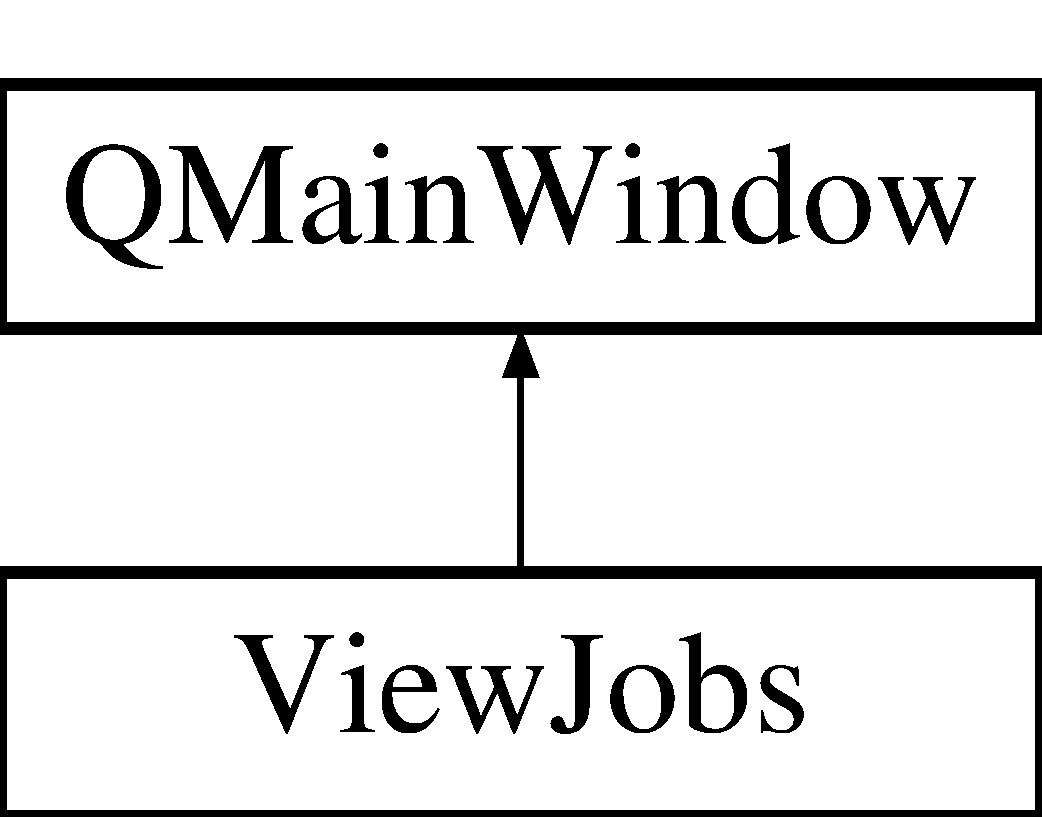
\includegraphics[height=2.000000cm]{class_view_jobs}
\end{center}
\end{figure}
\subsection*{Signals}
\begin{DoxyCompactItemize}
\item 
\mbox{\Hypertarget{class_view_jobs_a6fe28a8ba9112250d4337d02e0abedbd}\label{class_view_jobs_a6fe28a8ba9112250d4337d02e0abedbd}} 
void {\bfseries sig\+Show\+Event} ()
\end{DoxyCompactItemize}
\subsection*{Public Member Functions}
\begin{DoxyCompactItemize}
\item 
\mbox{\hyperlink{class_view_jobs_ac78f48cc812a0348a233f33dc78a71cc}{View\+Jobs}} (Q\+String window\+Title, \mbox{\hyperlink{classpsql}{psql}} $\ast$pg, Q\+Widget $\ast$parent=0)
\begin{DoxyCompactList}\small\item\em \mbox{\hyperlink{class_view_jobs}{View\+Jobs}} The \mbox{\hyperlink{class_view_jobs}{View\+Jobs}} class constructor. \end{DoxyCompactList}\item 
\mbox{\Hypertarget{class_view_jobs_af97593f0db01caee0febfe774a823e9c}\label{class_view_jobs_af97593f0db01caee0febfe774a823e9c}} 
void \mbox{\hyperlink{class_view_jobs_af97593f0db01caee0febfe774a823e9c}{get\+Applications}} ()
\begin{DoxyCompactList}\small\item\em \mbox{\hyperlink{class_view_jobs_af97593f0db01caee0febfe774a823e9c}{View\+Jobs\+::get\+Applications}} Fills the combo\+Box\+Application\+ID with all application I\+Ds in the database. \end{DoxyCompactList}\item 
void \mbox{\hyperlink{class_view_jobs_ae9c1c806aa1dd5082b38a1dc9cbec39e}{get\+Application}} (int app\+ID)
\begin{DoxyCompactList}\small\item\em \mbox{\hyperlink{class_view_jobs_ae9c1c806aa1dd5082b38a1dc9cbec39e}{View\+Jobs\+::get\+Application}} Fills the window with information based on the application ID. \end{DoxyCompactList}\item 
void \mbox{\hyperlink{class_view_jobs_acd43a8c32ab9bca7e40ecc99e51da9b8}{set\+Application\+ID}} (int new\+ID)
\begin{DoxyCompactList}\small\item\em \mbox{\hyperlink{class_view_jobs_acd43a8c32ab9bca7e40ecc99e51da9b8}{View\+Jobs\+::set\+Application\+ID}} sets a new application ID. Note that this does N\+OT change the ID of the current application. \end{DoxyCompactList}\item 
void \mbox{\hyperlink{class_view_jobs_abfe1969197cde57ea049c1b7d91cd4f5}{set\+Title}} (Q\+String new\+Title)
\begin{DoxyCompactList}\small\item\em \mbox{\hyperlink{class_view_jobs_abfe1969197cde57ea049c1b7d91cd4f5}{View\+Jobs\+::set\+Title}} Sets a new job title. \end{DoxyCompactList}\item 
void \mbox{\hyperlink{class_view_jobs_a596246d07be66a5aeaf14ff8e5649290}{set\+Company}} (Q\+String new\+Company)
\begin{DoxyCompactList}\small\item\em \mbox{\hyperlink{class_view_jobs_a596246d07be66a5aeaf14ff8e5649290}{View\+Jobs\+::set\+Company}} Sets a new employer company name. \end{DoxyCompactList}\item 
void \mbox{\hyperlink{class_view_jobs_ad89218b37af85cac9ce6c346efb57e56}{set\+City\+ID}} (int new\+Town\+ID)
\begin{DoxyCompactList}\small\item\em \mbox{\hyperlink{class_view_jobs_ad89218b37af85cac9ce6c346efb57e56}{View\+Jobs\+::set\+City\+ID}} Sets a new city ID. \end{DoxyCompactList}\item 
void \mbox{\hyperlink{class_view_jobs_a55943415fd91377d5f701f7074ba58d6}{set\+Status\+ID}} (int new\+Status\+ID)
\begin{DoxyCompactList}\small\item\em \mbox{\hyperlink{class_view_jobs_a55943415fd91377d5f701f7074ba58d6}{View\+Jobs\+::set\+Status\+ID}} Sets a new status ID for the current job. \end{DoxyCompactList}\item 
void \mbox{\hyperlink{class_view_jobs_a7574794410eb40956f343976de97221f}{set\+Date}} (Q\+String new\+Date)
\begin{DoxyCompactList}\small\item\em \mbox{\hyperlink{class_view_jobs_a7574794410eb40956f343976de97221f}{View\+Jobs\+::set\+Date}} Sets a new application deadline for the job application. \end{DoxyCompactList}\item 
void \mbox{\hyperlink{class_view_jobs_a53bdfabaf2b442841d676f42ebbf975f}{set\+Motivation}} (Q\+String new\+Motivation)
\begin{DoxyCompactList}\small\item\em \mbox{\hyperlink{class_view_jobs_a53bdfabaf2b442841d676f42ebbf975f}{View\+Jobs\+::set\+Motivation}} Sets the new job motivation. \end{DoxyCompactList}\item 
int \mbox{\hyperlink{class_view_jobs_a086650882ad80acb4074cf697f8cddcb}{get\+Application\+ID}} ()
\begin{DoxyCompactList}\small\item\em \mbox{\hyperlink{class_view_jobs_a086650882ad80acb4074cf697f8cddcb}{View\+Jobs\+::get\+Application\+ID}} Gets the current application ID. \end{DoxyCompactList}\item 
Q\+String \mbox{\hyperlink{class_view_jobs_ae78f119d37c77a9e3e457ecfd78d7de3}{get\+Title}} ()
\begin{DoxyCompactList}\small\item\em \mbox{\hyperlink{class_view_jobs_ae78f119d37c77a9e3e457ecfd78d7de3}{View\+Jobs\+::get\+Title}} Gets the application ID. \end{DoxyCompactList}\item 
Q\+String \mbox{\hyperlink{class_view_jobs_a88d7c0a7a79bc7a7e02b524587983bf8}{get\+Company}} ()
\begin{DoxyCompactList}\small\item\em \mbox{\hyperlink{class_view_jobs_a88d7c0a7a79bc7a7e02b524587983bf8}{View\+Jobs\+::get\+Company}} Gets the current employer company. \end{DoxyCompactList}\item 
int \mbox{\hyperlink{class_view_jobs_adcafeca350b21a033aa630e042ee7947}{get\+City\+ID}} ()
\begin{DoxyCompactList}\small\item\em \mbox{\hyperlink{class_view_jobs_adcafeca350b21a033aa630e042ee7947}{View\+Jobs\+::get\+City\+ID}} Gets the ID of the city where the job is located. \end{DoxyCompactList}\item 
int \mbox{\hyperlink{class_view_jobs_a91696fde9f0a663bae929390aac8324b}{get\+Status\+ID}} ()
\begin{DoxyCompactList}\small\item\em \mbox{\hyperlink{class_view_jobs_a91696fde9f0a663bae929390aac8324b}{View\+Jobs\+::get\+Status\+ID}} Gets the current status ID of the job application. \end{DoxyCompactList}\item 
Q\+String \mbox{\hyperlink{class_view_jobs_af046f9201cc6031e070b4f9b613a35f9}{get\+Date}} ()
\begin{DoxyCompactList}\small\item\em \mbox{\hyperlink{class_view_jobs_af046f9201cc6031e070b4f9b613a35f9}{View\+Jobs\+::get\+Date}} Gets the current application\textquotesingle{}s dealine. \end{DoxyCompactList}\item 
\mbox{\Hypertarget{class_view_jobs_a6cf031afcc4a09dfca54044fdf8c4f7b}\label{class_view_jobs_a6cf031afcc4a09dfca54044fdf8c4f7b}} 
void \mbox{\hyperlink{class_view_jobs_a6cf031afcc4a09dfca54044fdf8c4f7b}{get\+City\+I\+Ds}} ()
\begin{DoxyCompactList}\small\item\em \mbox{\hyperlink{class_view_jobs_a6cf031afcc4a09dfca54044fdf8c4f7b}{View\+Jobs\+::get\+City\+I\+Ds}} Fills the combo\+Box\+Town\+ID with all city I\+Ds that exist in the databse. \end{DoxyCompactList}\item 
Q\+String \mbox{\hyperlink{class_view_jobs_a238ec5365ef2c39baa97670769dfedca}{get\+Motivation}} ()
\begin{DoxyCompactList}\small\item\em \mbox{\hyperlink{class_view_jobs_a238ec5365ef2c39baa97670769dfedca}{View\+Jobs\+::get\+Motivation}} Gets the current job motivation. \end{DoxyCompactList}\item 
\mbox{\Hypertarget{class_view_jobs_adabe196e81c74d17c436de1a6ea12099}\label{class_view_jobs_adabe196e81c74d17c436de1a6ea12099}} 
void \mbox{\hyperlink{class_view_jobs_adabe196e81c74d17c436de1a6ea12099}{get\+Status\+I\+Ds}} ()
\begin{DoxyCompactList}\small\item\em \mbox{\hyperlink{class_view_jobs_adabe196e81c74d17c436de1a6ea12099}{View\+Jobs\+::get\+Status\+I\+Ds}} Fills the combo\+Box\+Status\+ID with all status I\+Ds that exist in the database. \end{DoxyCompactList}\item 
bool \mbox{\hyperlink{class_view_jobs_a5f75b45d28ce7f4a8050ce9ce0f44350}{is\+Changed}} ()
\begin{DoxyCompactList}\small\item\em \mbox{\hyperlink{class_view_jobs_a5f75b45d28ce7f4a8050ce9ce0f44350}{View\+Jobs\+::is\+Changed}} Checks if there have been any unsaved changes to the current record. \end{DoxyCompactList}\item 
void \mbox{\hyperlink{class_view_jobs_a3cba868c6deadaf4b35c18982f7ec35e}{set\+Changed}} (bool change)
\begin{DoxyCompactList}\small\item\em \mbox{\hyperlink{class_view_jobs_a3cba868c6deadaf4b35c18982f7ec35e}{View\+Jobs\+::set\+Changed}} Sets the changed variable to true if there are unsaved changes, and false if those changes have been saved. \end{DoxyCompactList}\item 
void \mbox{\hyperlink{class_view_jobs_a832503ca9eb4e4bf79c2fb48a59141aa}{close\+Event}} (Q\+Close\+Event $\ast$event) override
\begin{DoxyCompactList}\small\item\em \mbox{\hyperlink{class_view_jobs_a832503ca9eb4e4bf79c2fb48a59141aa}{View\+Jobs\+::close\+Event}} Code to be executed when the user has ordered the window to be closed. \end{DoxyCompactList}\item 
\mbox{\Hypertarget{class_view_jobs_a50f3a52f43e097d46e106e0aa31e9eb4}\label{class_view_jobs_a50f3a52f43e097d46e106e0aa31e9eb4}} 
void {\bfseries show\+Event} (Q\+Show\+Event $\ast$) override
\end{DoxyCompactItemize}


\subsection{Detailed Description}
The \mbox{\hyperlink{class_view_jobs}{View\+Jobs}} class. 

\subsection{Constructor \& Destructor Documentation}
\mbox{\Hypertarget{class_view_jobs_ac78f48cc812a0348a233f33dc78a71cc}\label{class_view_jobs_ac78f48cc812a0348a233f33dc78a71cc}} 
\index{View\+Jobs@{View\+Jobs}!View\+Jobs@{View\+Jobs}}
\index{View\+Jobs@{View\+Jobs}!View\+Jobs@{View\+Jobs}}
\subsubsection{\texorpdfstring{View\+Jobs()}{ViewJobs()}}
{\footnotesize\ttfamily View\+Jobs\+::\+View\+Jobs (\begin{DoxyParamCaption}\item[{Q\+String}]{window\+Title,  }\item[{\mbox{\hyperlink{classpsql}{psql}} $\ast$}]{pg,  }\item[{Q\+Widget $\ast$}]{parent = {\ttfamily 0} }\end{DoxyParamCaption})\hspace{0.3cm}{\ttfamily [explicit]}}



\mbox{\hyperlink{class_view_jobs}{View\+Jobs}} The \mbox{\hyperlink{class_view_jobs}{View\+Jobs}} class constructor. 


\begin{DoxyParams}{Parameters}
{\em window\+Title} & The name to be used as titles in windows and message boxes. \\
\hline
{\em pg} & A pointer to the Postgre\+S\+QL database class. \\
\hline
{\em parent} & \\
\hline
\end{DoxyParams}


\subsection{Member Function Documentation}
\mbox{\Hypertarget{class_view_jobs_a832503ca9eb4e4bf79c2fb48a59141aa}\label{class_view_jobs_a832503ca9eb4e4bf79c2fb48a59141aa}} 
\index{View\+Jobs@{View\+Jobs}!close\+Event@{close\+Event}}
\index{close\+Event@{close\+Event}!View\+Jobs@{View\+Jobs}}
\subsubsection{\texorpdfstring{close\+Event()}{closeEvent()}}
{\footnotesize\ttfamily void View\+Jobs\+::close\+Event (\begin{DoxyParamCaption}\item[{Q\+Close\+Event $\ast$}]{event }\end{DoxyParamCaption})\hspace{0.3cm}{\ttfamily [override]}}



\mbox{\hyperlink{class_view_jobs_a832503ca9eb4e4bf79c2fb48a59141aa}{View\+Jobs\+::close\+Event}} Code to be executed when the user has ordered the window to be closed. 


\begin{DoxyParams}{Parameters}
{\em event} & No help available, sorry \\
\hline
\end{DoxyParams}
\mbox{\Hypertarget{class_view_jobs_ae9c1c806aa1dd5082b38a1dc9cbec39e}\label{class_view_jobs_ae9c1c806aa1dd5082b38a1dc9cbec39e}} 
\index{View\+Jobs@{View\+Jobs}!get\+Application@{get\+Application}}
\index{get\+Application@{get\+Application}!View\+Jobs@{View\+Jobs}}
\subsubsection{\texorpdfstring{get\+Application()}{getApplication()}}
{\footnotesize\ttfamily void View\+Jobs\+::get\+Application (\begin{DoxyParamCaption}\item[{int}]{app\+ID }\end{DoxyParamCaption})}



\mbox{\hyperlink{class_view_jobs_ae9c1c806aa1dd5082b38a1dc9cbec39e}{View\+Jobs\+::get\+Application}} Fills the window with information based on the application ID. 


\begin{DoxyParams}{Parameters}
{\em app\+ID} & the application ID to be used. \\
\hline
\end{DoxyParams}
\mbox{\Hypertarget{class_view_jobs_a086650882ad80acb4074cf697f8cddcb}\label{class_view_jobs_a086650882ad80acb4074cf697f8cddcb}} 
\index{View\+Jobs@{View\+Jobs}!get\+Application\+ID@{get\+Application\+ID}}
\index{get\+Application\+ID@{get\+Application\+ID}!View\+Jobs@{View\+Jobs}}
\subsubsection{\texorpdfstring{get\+Application\+I\+D()}{getApplicationID()}}
{\footnotesize\ttfamily int View\+Jobs\+::get\+Application\+ID (\begin{DoxyParamCaption}{ }\end{DoxyParamCaption})}



\mbox{\hyperlink{class_view_jobs_a086650882ad80acb4074cf697f8cddcb}{View\+Jobs\+::get\+Application\+ID}} Gets the current application ID. 

\begin{DoxyReturn}{Returns}
The current application ID. 
\end{DoxyReturn}
\mbox{\Hypertarget{class_view_jobs_adcafeca350b21a033aa630e042ee7947}\label{class_view_jobs_adcafeca350b21a033aa630e042ee7947}} 
\index{View\+Jobs@{View\+Jobs}!get\+City\+ID@{get\+City\+ID}}
\index{get\+City\+ID@{get\+City\+ID}!View\+Jobs@{View\+Jobs}}
\subsubsection{\texorpdfstring{get\+City\+I\+D()}{getCityID()}}
{\footnotesize\ttfamily int View\+Jobs\+::get\+City\+ID (\begin{DoxyParamCaption}{ }\end{DoxyParamCaption})}



\mbox{\hyperlink{class_view_jobs_adcafeca350b21a033aa630e042ee7947}{View\+Jobs\+::get\+City\+ID}} Gets the ID of the city where the job is located. 

\begin{DoxyReturn}{Returns}
the ID of the city where the job is located. 
\end{DoxyReturn}
\mbox{\Hypertarget{class_view_jobs_a88d7c0a7a79bc7a7e02b524587983bf8}\label{class_view_jobs_a88d7c0a7a79bc7a7e02b524587983bf8}} 
\index{View\+Jobs@{View\+Jobs}!get\+Company@{get\+Company}}
\index{get\+Company@{get\+Company}!View\+Jobs@{View\+Jobs}}
\subsubsection{\texorpdfstring{get\+Company()}{getCompany()}}
{\footnotesize\ttfamily Q\+String View\+Jobs\+::get\+Company (\begin{DoxyParamCaption}{ }\end{DoxyParamCaption})}



\mbox{\hyperlink{class_view_jobs_a88d7c0a7a79bc7a7e02b524587983bf8}{View\+Jobs\+::get\+Company}} Gets the current employer company. 

\begin{DoxyReturn}{Returns}
the current company. 
\end{DoxyReturn}
\mbox{\Hypertarget{class_view_jobs_af046f9201cc6031e070b4f9b613a35f9}\label{class_view_jobs_af046f9201cc6031e070b4f9b613a35f9}} 
\index{View\+Jobs@{View\+Jobs}!get\+Date@{get\+Date}}
\index{get\+Date@{get\+Date}!View\+Jobs@{View\+Jobs}}
\subsubsection{\texorpdfstring{get\+Date()}{getDate()}}
{\footnotesize\ttfamily Q\+String View\+Jobs\+::get\+Date (\begin{DoxyParamCaption}{ }\end{DoxyParamCaption})}



\mbox{\hyperlink{class_view_jobs_af046f9201cc6031e070b4f9b613a35f9}{View\+Jobs\+::get\+Date}} Gets the current application\textquotesingle{}s dealine. 

\begin{DoxyReturn}{Returns}
The deadline of the current application. 
\end{DoxyReturn}
\mbox{\Hypertarget{class_view_jobs_a238ec5365ef2c39baa97670769dfedca}\label{class_view_jobs_a238ec5365ef2c39baa97670769dfedca}} 
\index{View\+Jobs@{View\+Jobs}!get\+Motivation@{get\+Motivation}}
\index{get\+Motivation@{get\+Motivation}!View\+Jobs@{View\+Jobs}}
\subsubsection{\texorpdfstring{get\+Motivation()}{getMotivation()}}
{\footnotesize\ttfamily Q\+String View\+Jobs\+::get\+Motivation (\begin{DoxyParamCaption}{ }\end{DoxyParamCaption})}



\mbox{\hyperlink{class_view_jobs_a238ec5365ef2c39baa97670769dfedca}{View\+Jobs\+::get\+Motivation}} Gets the current job motivation. 

\begin{DoxyReturn}{Returns}
A string containing what motivated the user to apply for this job. 
\end{DoxyReturn}
\mbox{\Hypertarget{class_view_jobs_a91696fde9f0a663bae929390aac8324b}\label{class_view_jobs_a91696fde9f0a663bae929390aac8324b}} 
\index{View\+Jobs@{View\+Jobs}!get\+Status\+ID@{get\+Status\+ID}}
\index{get\+Status\+ID@{get\+Status\+ID}!View\+Jobs@{View\+Jobs}}
\subsubsection{\texorpdfstring{get\+Status\+I\+D()}{getStatusID()}}
{\footnotesize\ttfamily int View\+Jobs\+::get\+Status\+ID (\begin{DoxyParamCaption}{ }\end{DoxyParamCaption})}



\mbox{\hyperlink{class_view_jobs_a91696fde9f0a663bae929390aac8324b}{View\+Jobs\+::get\+Status\+ID}} Gets the current status ID of the job application. 

\begin{DoxyReturn}{Returns}
the application\textquotesingle{}s current status ID. 
\end{DoxyReturn}
\mbox{\Hypertarget{class_view_jobs_ae78f119d37c77a9e3e457ecfd78d7de3}\label{class_view_jobs_ae78f119d37c77a9e3e457ecfd78d7de3}} 
\index{View\+Jobs@{View\+Jobs}!get\+Title@{get\+Title}}
\index{get\+Title@{get\+Title}!View\+Jobs@{View\+Jobs}}
\subsubsection{\texorpdfstring{get\+Title()}{getTitle()}}
{\footnotesize\ttfamily Q\+String View\+Jobs\+::get\+Title (\begin{DoxyParamCaption}{ }\end{DoxyParamCaption})}



\mbox{\hyperlink{class_view_jobs_ae78f119d37c77a9e3e457ecfd78d7de3}{View\+Jobs\+::get\+Title}} Gets the application ID. 

\begin{DoxyReturn}{Returns}
the current title. 
\end{DoxyReturn}
\mbox{\Hypertarget{class_view_jobs_a5f75b45d28ce7f4a8050ce9ce0f44350}\label{class_view_jobs_a5f75b45d28ce7f4a8050ce9ce0f44350}} 
\index{View\+Jobs@{View\+Jobs}!is\+Changed@{is\+Changed}}
\index{is\+Changed@{is\+Changed}!View\+Jobs@{View\+Jobs}}
\subsubsection{\texorpdfstring{is\+Changed()}{isChanged()}}
{\footnotesize\ttfamily bool View\+Jobs\+::is\+Changed (\begin{DoxyParamCaption}{ }\end{DoxyParamCaption})}



\mbox{\hyperlink{class_view_jobs_a5f75b45d28ce7f4a8050ce9ce0f44350}{View\+Jobs\+::is\+Changed}} Checks if there have been any unsaved changes to the current record. 

\begin{DoxyReturn}{Returns}
True if there are unsaved changes and false otherwise. 
\end{DoxyReturn}
\mbox{\Hypertarget{class_view_jobs_acd43a8c32ab9bca7e40ecc99e51da9b8}\label{class_view_jobs_acd43a8c32ab9bca7e40ecc99e51da9b8}} 
\index{View\+Jobs@{View\+Jobs}!set\+Application\+ID@{set\+Application\+ID}}
\index{set\+Application\+ID@{set\+Application\+ID}!View\+Jobs@{View\+Jobs}}
\subsubsection{\texorpdfstring{set\+Application\+I\+D()}{setApplicationID()}}
{\footnotesize\ttfamily void View\+Jobs\+::set\+Application\+ID (\begin{DoxyParamCaption}\item[{int}]{new\+ID }\end{DoxyParamCaption})}



\mbox{\hyperlink{class_view_jobs_acd43a8c32ab9bca7e40ecc99e51da9b8}{View\+Jobs\+::set\+Application\+ID}} sets a new application ID. Note that this does N\+OT change the ID of the current application. 


\begin{DoxyParams}{Parameters}
{\em new\+ID} & the new ID. \\
\hline
\end{DoxyParams}
\mbox{\Hypertarget{class_view_jobs_a3cba868c6deadaf4b35c18982f7ec35e}\label{class_view_jobs_a3cba868c6deadaf4b35c18982f7ec35e}} 
\index{View\+Jobs@{View\+Jobs}!set\+Changed@{set\+Changed}}
\index{set\+Changed@{set\+Changed}!View\+Jobs@{View\+Jobs}}
\subsubsection{\texorpdfstring{set\+Changed()}{setChanged()}}
{\footnotesize\ttfamily void View\+Jobs\+::set\+Changed (\begin{DoxyParamCaption}\item[{bool}]{change }\end{DoxyParamCaption})}



\mbox{\hyperlink{class_view_jobs_a3cba868c6deadaf4b35c18982f7ec35e}{View\+Jobs\+::set\+Changed}} Sets the changed variable to true if there are unsaved changes, and false if those changes have been saved. 


\begin{DoxyParams}{Parameters}
{\em change} & true if a record has been changed and false if that record has been saved \\
\hline
\end{DoxyParams}
\mbox{\Hypertarget{class_view_jobs_ad89218b37af85cac9ce6c346efb57e56}\label{class_view_jobs_ad89218b37af85cac9ce6c346efb57e56}} 
\index{View\+Jobs@{View\+Jobs}!set\+City\+ID@{set\+City\+ID}}
\index{set\+City\+ID@{set\+City\+ID}!View\+Jobs@{View\+Jobs}}
\subsubsection{\texorpdfstring{set\+City\+I\+D()}{setCityID()}}
{\footnotesize\ttfamily void View\+Jobs\+::set\+City\+ID (\begin{DoxyParamCaption}\item[{int}]{new\+Town\+ID }\end{DoxyParamCaption})}



\mbox{\hyperlink{class_view_jobs_ad89218b37af85cac9ce6c346efb57e56}{View\+Jobs\+::set\+City\+ID}} Sets a new city ID. 


\begin{DoxyParams}{Parameters}
{\em new\+Town\+ID} & the new city ID. \\
\hline
\end{DoxyParams}
\mbox{\Hypertarget{class_view_jobs_a596246d07be66a5aeaf14ff8e5649290}\label{class_view_jobs_a596246d07be66a5aeaf14ff8e5649290}} 
\index{View\+Jobs@{View\+Jobs}!set\+Company@{set\+Company}}
\index{set\+Company@{set\+Company}!View\+Jobs@{View\+Jobs}}
\subsubsection{\texorpdfstring{set\+Company()}{setCompany()}}
{\footnotesize\ttfamily void View\+Jobs\+::set\+Company (\begin{DoxyParamCaption}\item[{Q\+String}]{new\+Company }\end{DoxyParamCaption})}



\mbox{\hyperlink{class_view_jobs_a596246d07be66a5aeaf14ff8e5649290}{View\+Jobs\+::set\+Company}} Sets a new employer company name. 


\begin{DoxyParams}{Parameters}
{\em new\+Company} & the new company name. \\
\hline
\end{DoxyParams}
\mbox{\Hypertarget{class_view_jobs_a7574794410eb40956f343976de97221f}\label{class_view_jobs_a7574794410eb40956f343976de97221f}} 
\index{View\+Jobs@{View\+Jobs}!set\+Date@{set\+Date}}
\index{set\+Date@{set\+Date}!View\+Jobs@{View\+Jobs}}
\subsubsection{\texorpdfstring{set\+Date()}{setDate()}}
{\footnotesize\ttfamily void View\+Jobs\+::set\+Date (\begin{DoxyParamCaption}\item[{Q\+String}]{new\+Date }\end{DoxyParamCaption})}



\mbox{\hyperlink{class_view_jobs_a7574794410eb40956f343976de97221f}{View\+Jobs\+::set\+Date}} Sets a new application deadline for the job application. 


\begin{DoxyParams}{Parameters}
{\em new\+Date} & The new deadline for the current job application. \\
\hline
\end{DoxyParams}
\mbox{\Hypertarget{class_view_jobs_a53bdfabaf2b442841d676f42ebbf975f}\label{class_view_jobs_a53bdfabaf2b442841d676f42ebbf975f}} 
\index{View\+Jobs@{View\+Jobs}!set\+Motivation@{set\+Motivation}}
\index{set\+Motivation@{set\+Motivation}!View\+Jobs@{View\+Jobs}}
\subsubsection{\texorpdfstring{set\+Motivation()}{setMotivation()}}
{\footnotesize\ttfamily void View\+Jobs\+::set\+Motivation (\begin{DoxyParamCaption}\item[{Q\+String}]{new\+Motivation }\end{DoxyParamCaption})}



\mbox{\hyperlink{class_view_jobs_a53bdfabaf2b442841d676f42ebbf975f}{View\+Jobs\+::set\+Motivation}} Sets the new job motivation. 


\begin{DoxyParams}{Parameters}
{\em new\+Motivation} & A string explaining what motivated the user to apply for this job. \\
\hline
\end{DoxyParams}
\mbox{\Hypertarget{class_view_jobs_a55943415fd91377d5f701f7074ba58d6}\label{class_view_jobs_a55943415fd91377d5f701f7074ba58d6}} 
\index{View\+Jobs@{View\+Jobs}!set\+Status\+ID@{set\+Status\+ID}}
\index{set\+Status\+ID@{set\+Status\+ID}!View\+Jobs@{View\+Jobs}}
\subsubsection{\texorpdfstring{set\+Status\+I\+D()}{setStatusID()}}
{\footnotesize\ttfamily void View\+Jobs\+::set\+Status\+ID (\begin{DoxyParamCaption}\item[{int}]{new\+Status\+ID }\end{DoxyParamCaption})}



\mbox{\hyperlink{class_view_jobs_a55943415fd91377d5f701f7074ba58d6}{View\+Jobs\+::set\+Status\+ID}} Sets a new status ID for the current job. 


\begin{DoxyParams}{Parameters}
{\em new\+Status\+ID} & the ID of the application\textquotesingle{}s updated status. \\
\hline
\end{DoxyParams}
\mbox{\Hypertarget{class_view_jobs_abfe1969197cde57ea049c1b7d91cd4f5}\label{class_view_jobs_abfe1969197cde57ea049c1b7d91cd4f5}} 
\index{View\+Jobs@{View\+Jobs}!set\+Title@{set\+Title}}
\index{set\+Title@{set\+Title}!View\+Jobs@{View\+Jobs}}
\subsubsection{\texorpdfstring{set\+Title()}{setTitle()}}
{\footnotesize\ttfamily void View\+Jobs\+::set\+Title (\begin{DoxyParamCaption}\item[{Q\+String}]{new\+Title }\end{DoxyParamCaption})}



\mbox{\hyperlink{class_view_jobs_abfe1969197cde57ea049c1b7d91cd4f5}{View\+Jobs\+::set\+Title}} Sets a new job title. 


\begin{DoxyParams}{Parameters}
{\em new\+Title} & The new job/position title to be used. \\
\hline
\end{DoxyParams}


The documentation for this class was generated from the following files\+:\begin{DoxyCompactItemize}
\item 
viewjobs.\+h\item 
viewjobs.\+cpp\end{DoxyCompactItemize}

\chapter{File Documentation}
\hypertarget{newcity_8cpp}{}\section{newcity.\+cpp File Reference}
\label{newcity_8cpp}\index{newcity.\+cpp@{newcity.\+cpp}}
{\ttfamily \#include \char`\"{}newcity.\+h\char`\"{}}\newline
{\ttfamily \#include \char`\"{}ui\+\_\+newcity.\+h\char`\"{}}\newline
{\ttfamily \#include $<$Q\+Push\+Button$>$}\newline

\hypertarget{psql_8cpp}{}\section{psql.\+cpp File Reference}
\label{psql_8cpp}\index{psql.\+cpp@{psql.\+cpp}}
{\ttfamily \#include \char`\"{}psql.\+h\char`\"{}}\newline

%--- End generated contents ---

% Index
\backmatter
\newpage
\phantomsection
\clearemptydoublepage
\addcontentsline{toc}{chapter}{Index}
\printindex

\end{document}
